\chapter{Results}
\label{ch:results}
\epigraph{\emph{“Champions keep playing until they get it right.”}}{Billie Jean King}


It was introduced in \Sect{\ref{sec:strategy:strategy}}, in a brief way, the two different types of fits that can be performed to the recollected \ac{ATLAS} Run-2 data. Moreover, the numerous fitting strategies that need to be applied for each signal and in each signal region were derived and discussed in \Sect{\ref{sec:bkg:modeling}}.

In this chapter, the results obtained using the full Run-2 dataset are presented. First, in \Sect{\ref{sec:results:obs}}, in order to correctly present the results and to compute the fit p-values, the optimal binning is derived using \ac{MC} simulation. Finally, in \Sect{\ref{sec:results:results}}, the different fitting strategies are applied based on the \ac{BO} and \ac{SB} interpretations.






%%%%%%%%%%%%%%%%%%%%%%%%%%%%%%%%%%%%%%%%%%%%%%%%%%%%%%%%%%%%%%%%%%%%%%%%%%%%%%%%%%%%%%%%%%%%%%%%%%%%
%%%%%%%%%%%%%%%%%%%%%%%%%%%%%%%%%%%%%%%%%%%%%%%%%%%%%%%%%%%%%%%%%%%%%%%%%%%%%%%%%%%%%%%%%%%%%%%%%%%%
%%%%%%%%%%%%%%%%%%%%%%%%%%%%%%%%%%%%%%%%%%%%%%%%%%%%%%%%%%%%%%%%%%%%%%%%%%%%%%%%%%%%%%%%%%%%%%%%%%%%
%%%%%%%%%%%%%%%%%%%%%%%%%%%%%%%%%%%%%%%%%%%%%%%%%%%%%%%%%%%%%%%%%%%%%%%%%%%%%%%%%%%%%%%%%%%%%%%%%%%%
%%%%%%%%%%%%%%%%%%%%%%%%%%%%%%%%%%%%%%%%%%%%%%%%%%%%%%%%%%%%%%%%%%%%%%%%%%%%%%%%%%%%%%%%%%%%%%%%%%%%
%%%%%%%%%%%%%%%%%%%%%%%%%%%%%%%%%%%%%%%%%%%%%%%%%%%%%%%%%%%%%%%%%%%%%%%%%%%%%%%%%%%%%%%%%%%%%%%%%%%%
\section{Photon+jet invariant mass binning}
\label{sec:results:obs}


The \gammajet invariant mass, \myj, is the observable in the current analysis. In order to correctly display the results, a suitable binning needs to be chosen, being not too wide where bumps might not be visible, but also not too narrow that there is bin migration, due to the detector resolution on the mass.

\begin{figure}[ht!]
    \centering
    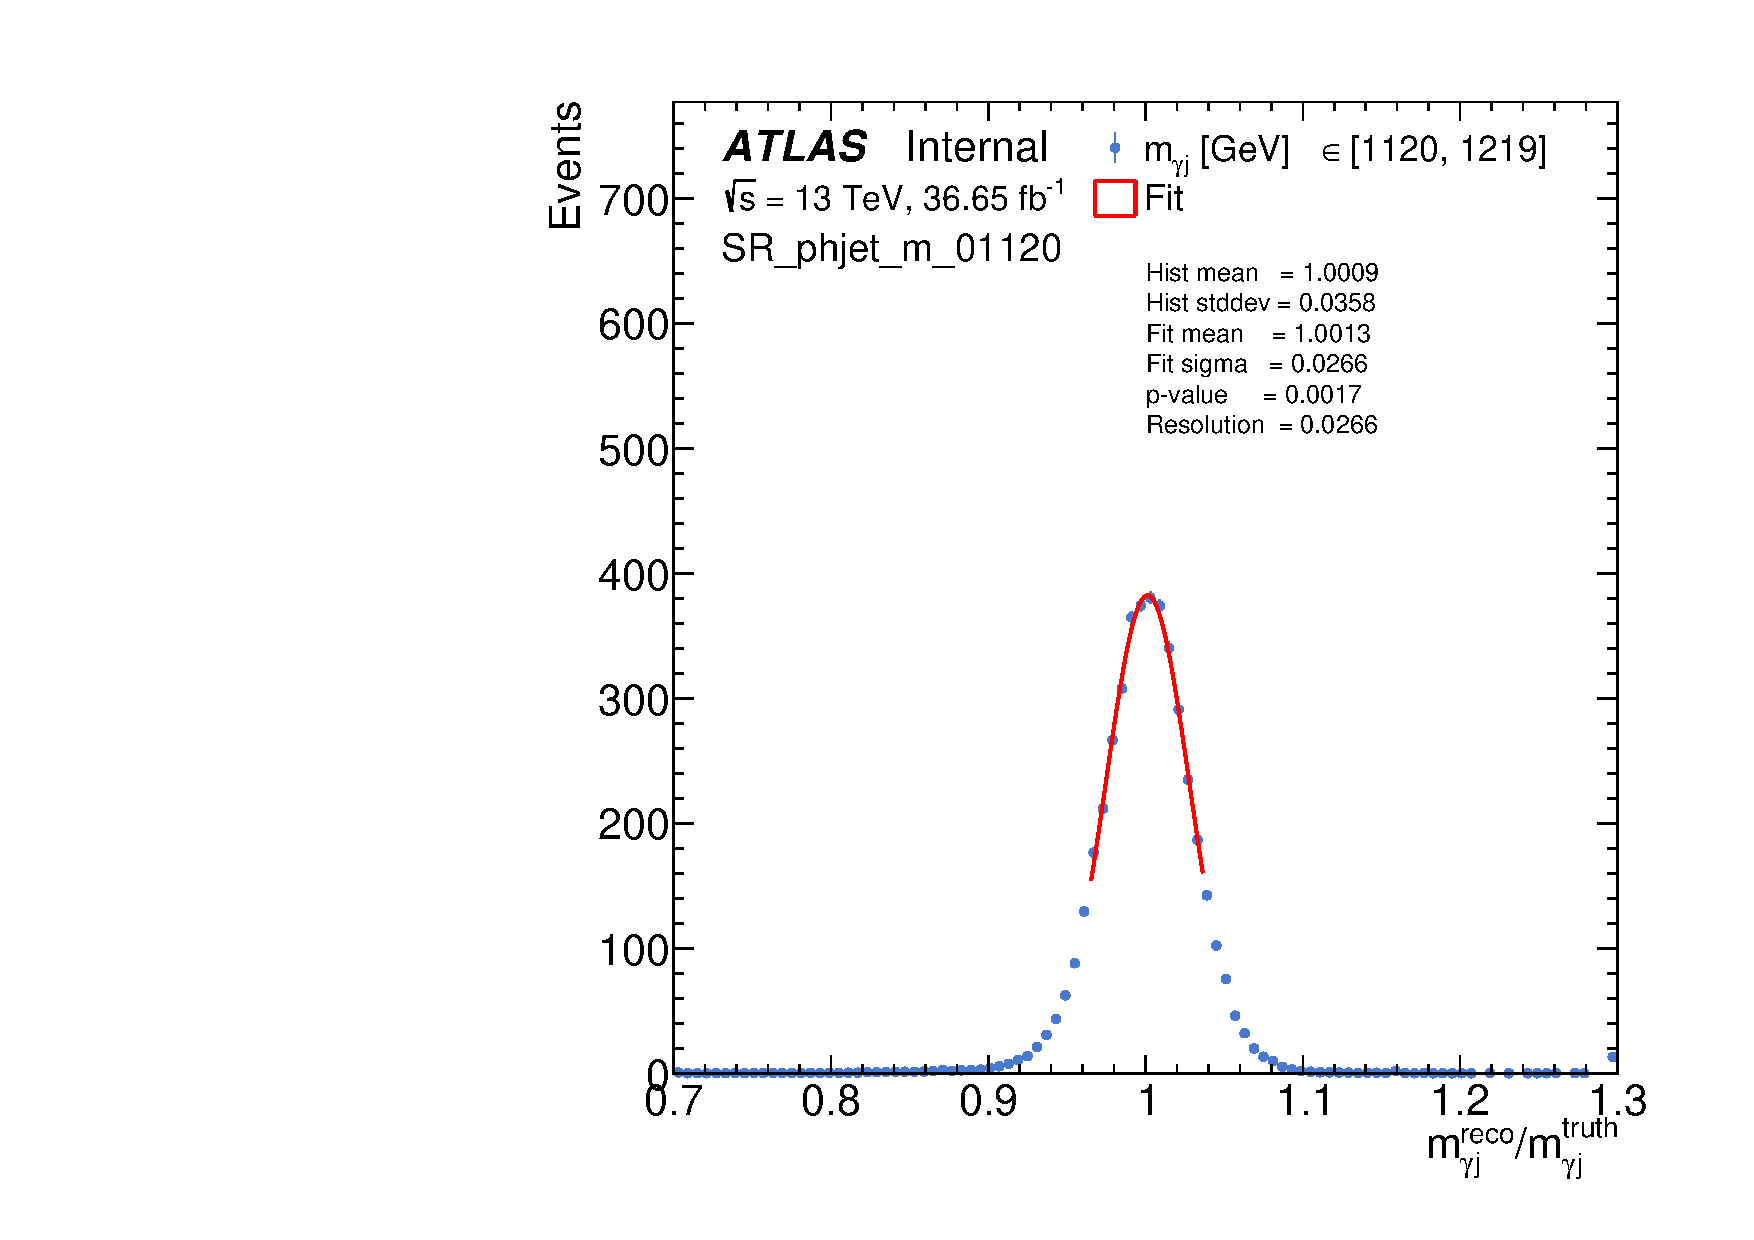
\includegraphics[width=0.32\linewidth]{5_resonances/results/myj_binning/distributions/can__phjet_m_over_phjet_truth_m__SR_phjet_m_01120}
    \hfill
    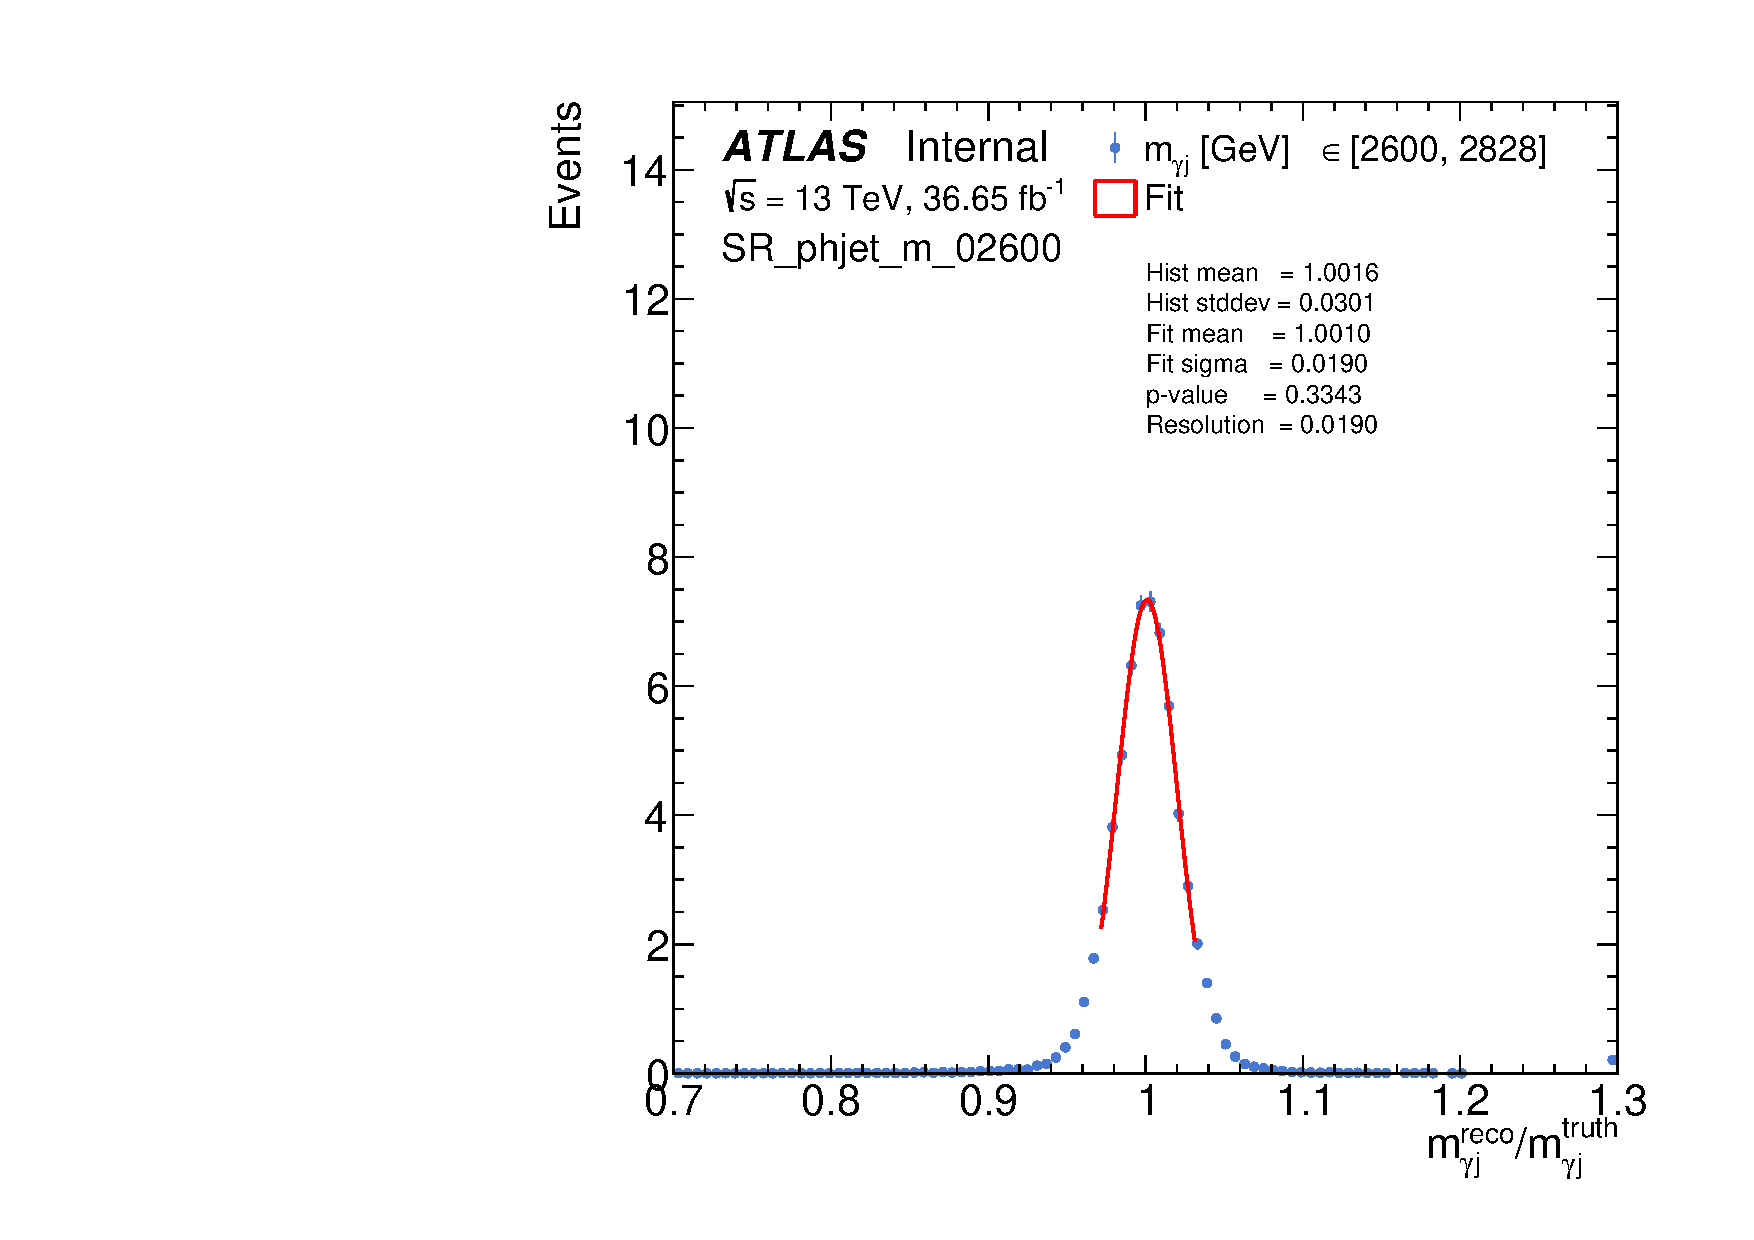
\includegraphics[width=0.32\linewidth]{5_resonances/results/myj_binning/distributions/can__phjet_m_over_phjet_truth_m__SR_phjet_m_02600}
    \hfill
    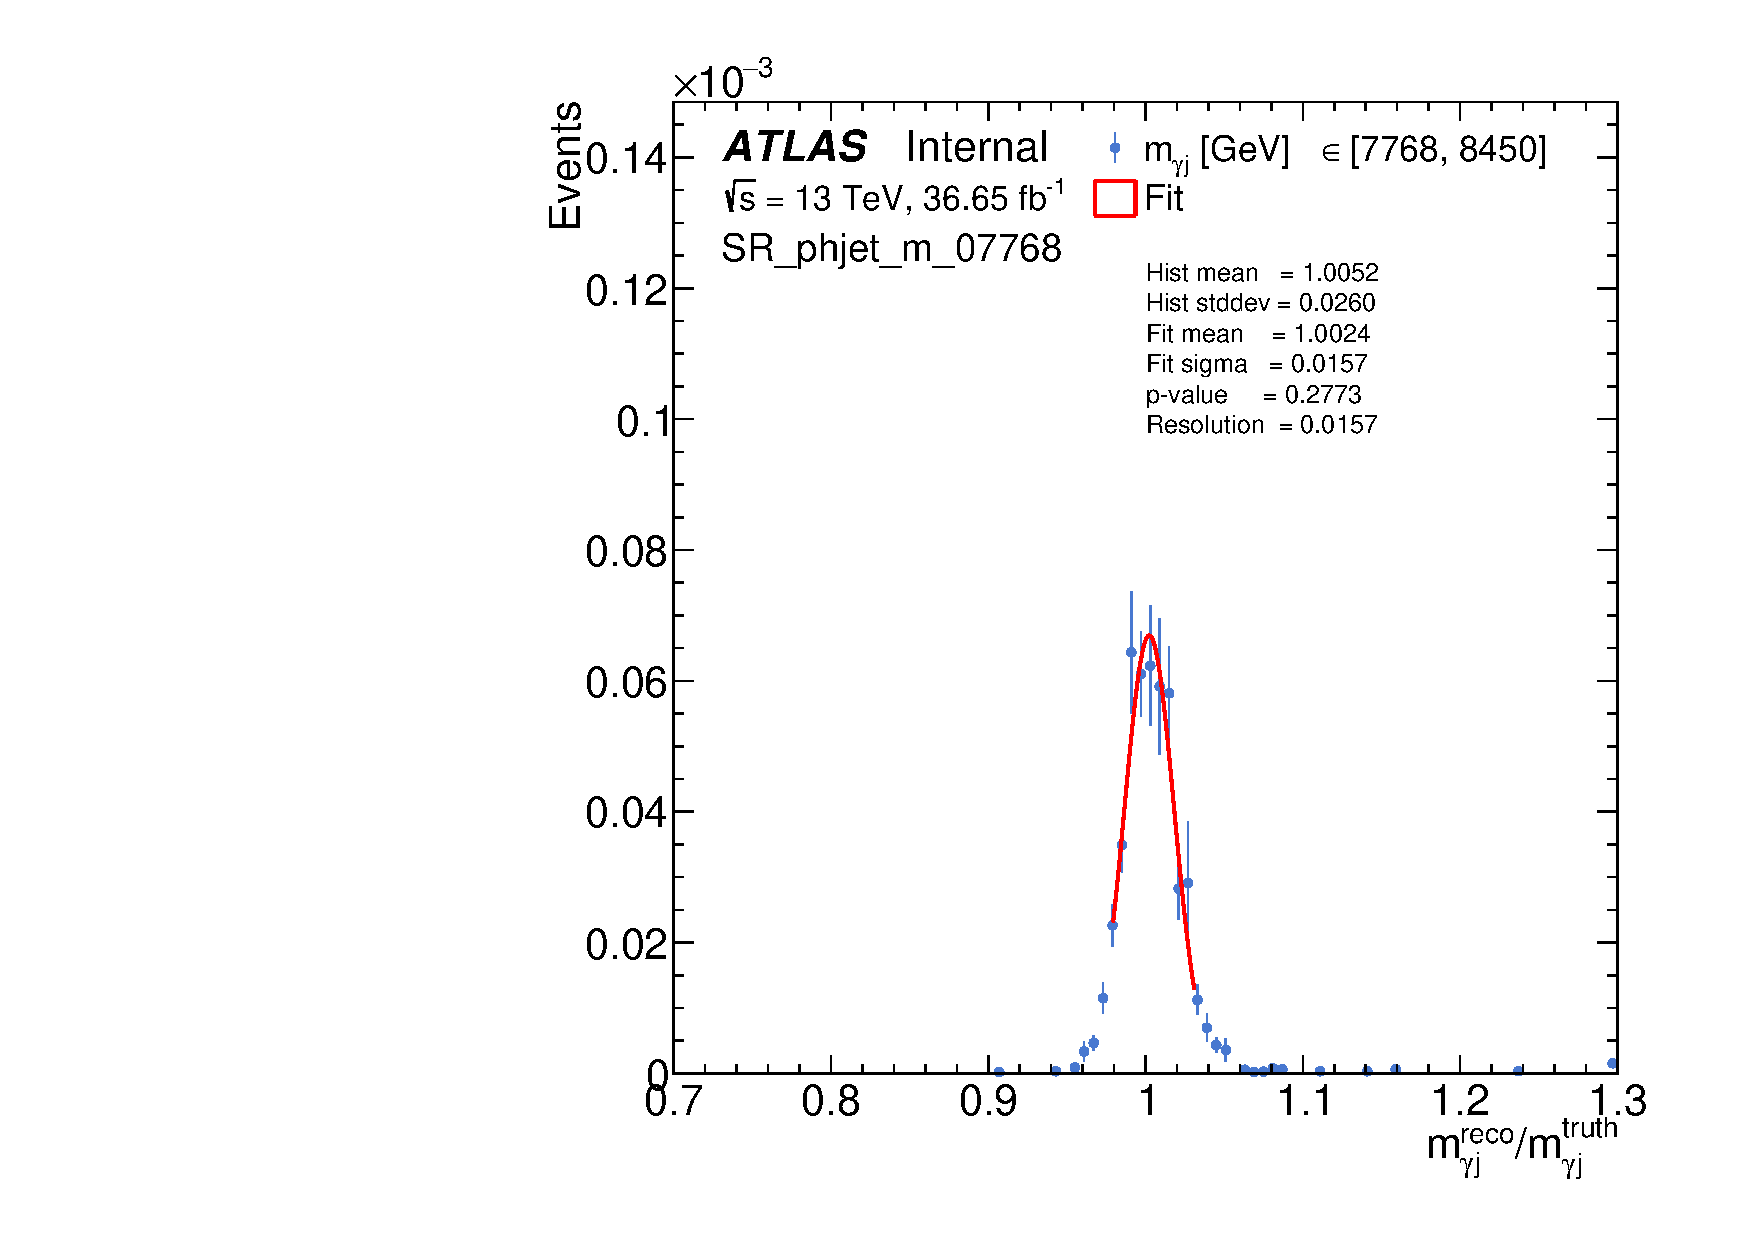
\includegraphics[width=0.32\linewidth]{5_resonances/results/myj_binning/distributions/can__phjet_m_over_phjet_truth_m__SR_phjet_m_07768}
    \caption{Selected \(\myj^{reco} / \myj^{truth}\) fits for the \myj binning studies. The distribution is shown with the blue dots while the gaussian fit with the red line. In all cases, the mean and standard deviation of the gaussian post-fit is shown.}
    \label{fig:results:obs:ratio_fits}
\end{figure}

\begin{figure}[ht!]
    \centering
    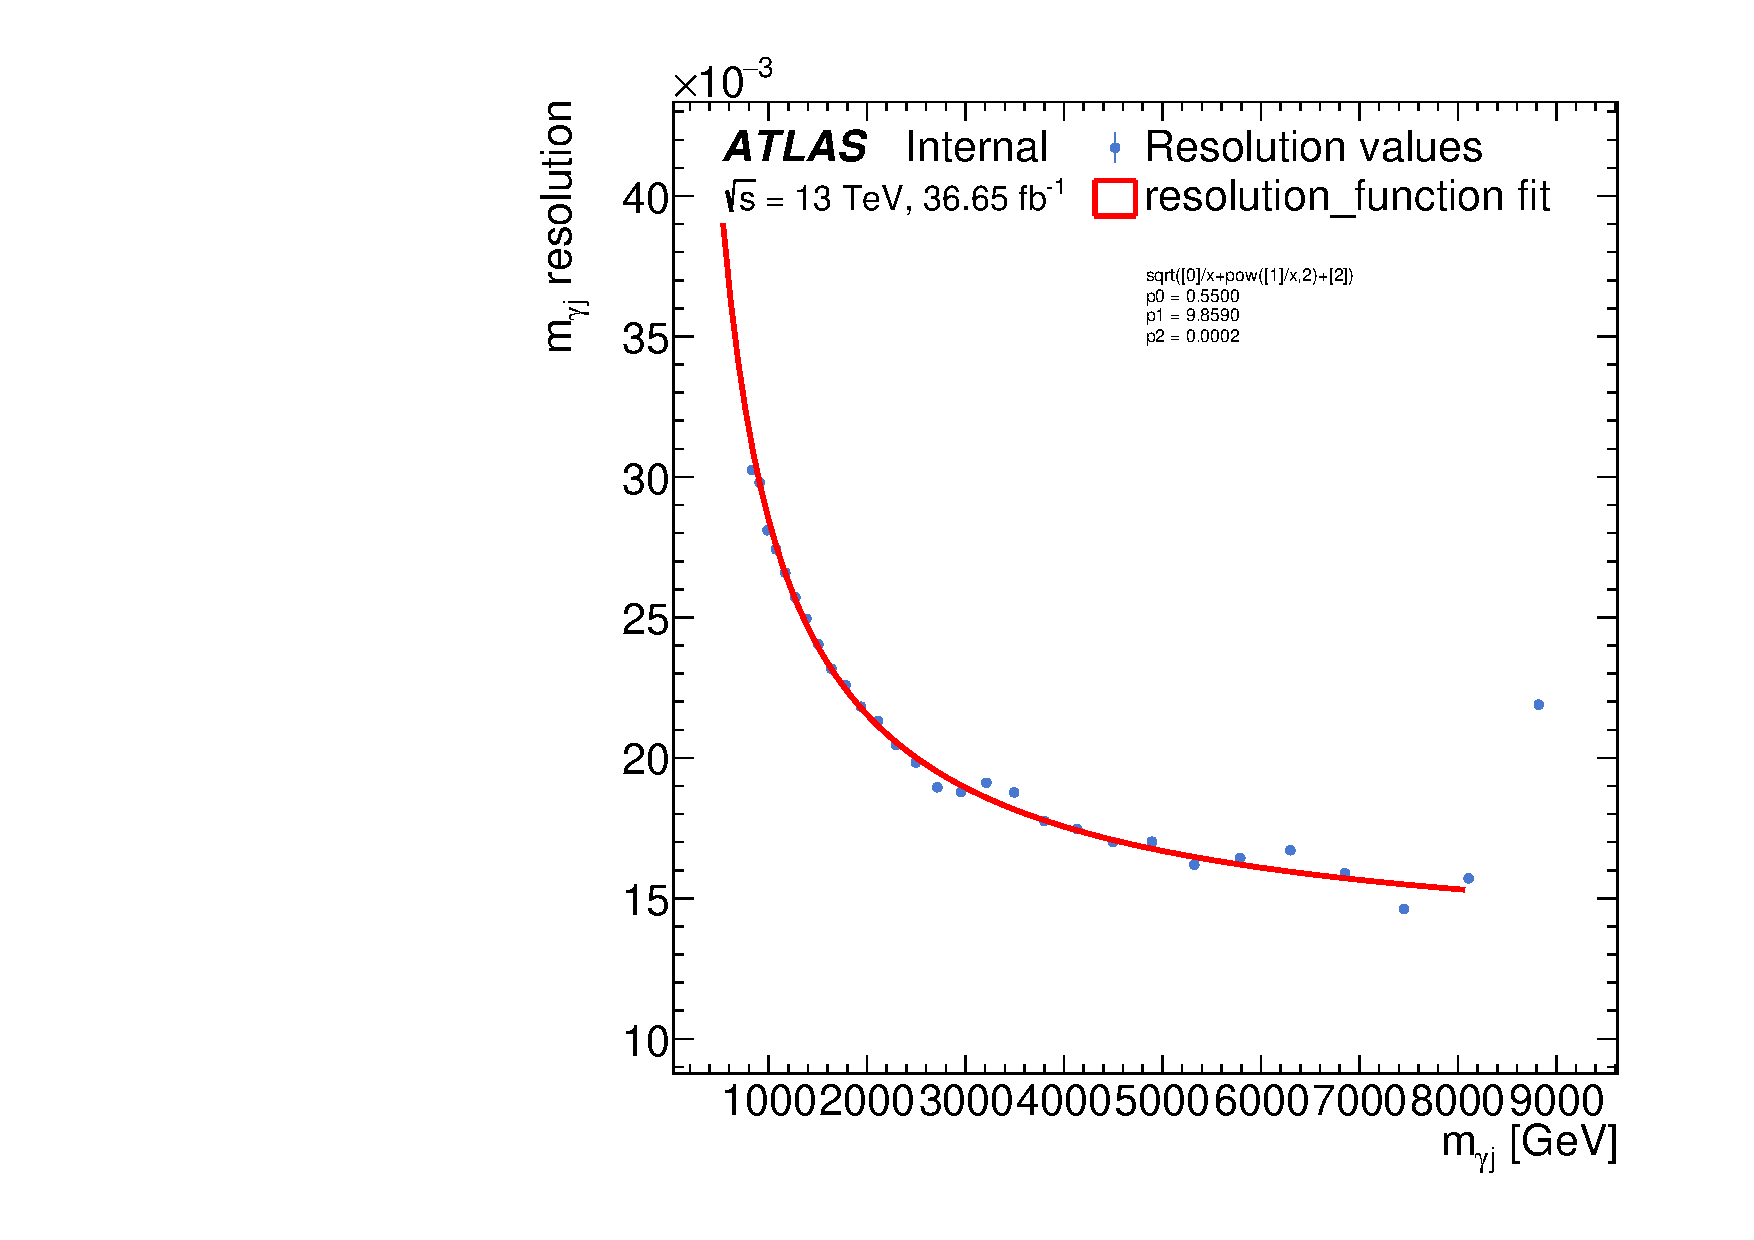
\includegraphics[width=0.7\linewidth]{5_resonances/results/myj_binning/resolution/can__phjet_m_over_phjet_truth_m_resolution__fit_resolution_function}
    \caption{\myj resolution values and fit using \Eqn{\ref{eq:results:obs:binning_resolution}}. The post-fit parameters are indicated in the figure where \(p_0 \equiv a\), \(p_1 \equiv b\) and \(p_2 \equiv c\). The fit has been performed excluding the last measured resolution value due to lack of statistics.}
    \label{fig:results:obs:resolution_curve}
\end{figure}

The binning should be wider than the detector resolution. In order to estimate the detector resolution, the \pythia \gammajet \ac{MC} simulation normalised to the 2015+2106 dataset is used. As a first step, the ratios \(\myj^{reco} / \myj^{truth}\) are computed in bins of \myj and for each bin a gaussian function \(g(\mu, \sigma)\) is fitted to the ratio, as shown in \Fig{\ref{fig:results:obs:ratio_fits}}, and the ratio \(\sigma / \mu\) corresponds to the resolution. The resulting set of resolution values are plotted as a function of \myj and a fit to it of the form
\begin{equation}
    \label{eq:results:obs:binning_resolution}
    \frac{\sigma}{\myj} = \sqrt{
        \frac{a}{\myj} +
        \left(\frac{b}{\myj}\right)^2 +
        c
    }
\end{equation}
is performed, shown in \Fig{\ref{fig:results:obs:resolution_curve}}. Finally, the \myj binning is calculated, starting at \(500~\gev\) up to \(10~\tev\), in an iterative fashion so that the bin-wdith is compatible with the resolution. The obtained bin-width as a function of \myj is shown in \Fig{\ref{fig:bkg_modeling:observable:results:binwidth}}, which shows a monotonically increasing nature, as expected. Finally, to validate that the binning resolution is in agreement with the detector one, in \Fig{\ref{fig:bkg_modeling:observable:results:resolution_comparison}}, a comparison between two is shown, from which excellent agreement is observed.

\begin{figure}[ht!]
    \centering
    \begin{subfigure}[h]{0.49\linewidth}
        \centering
        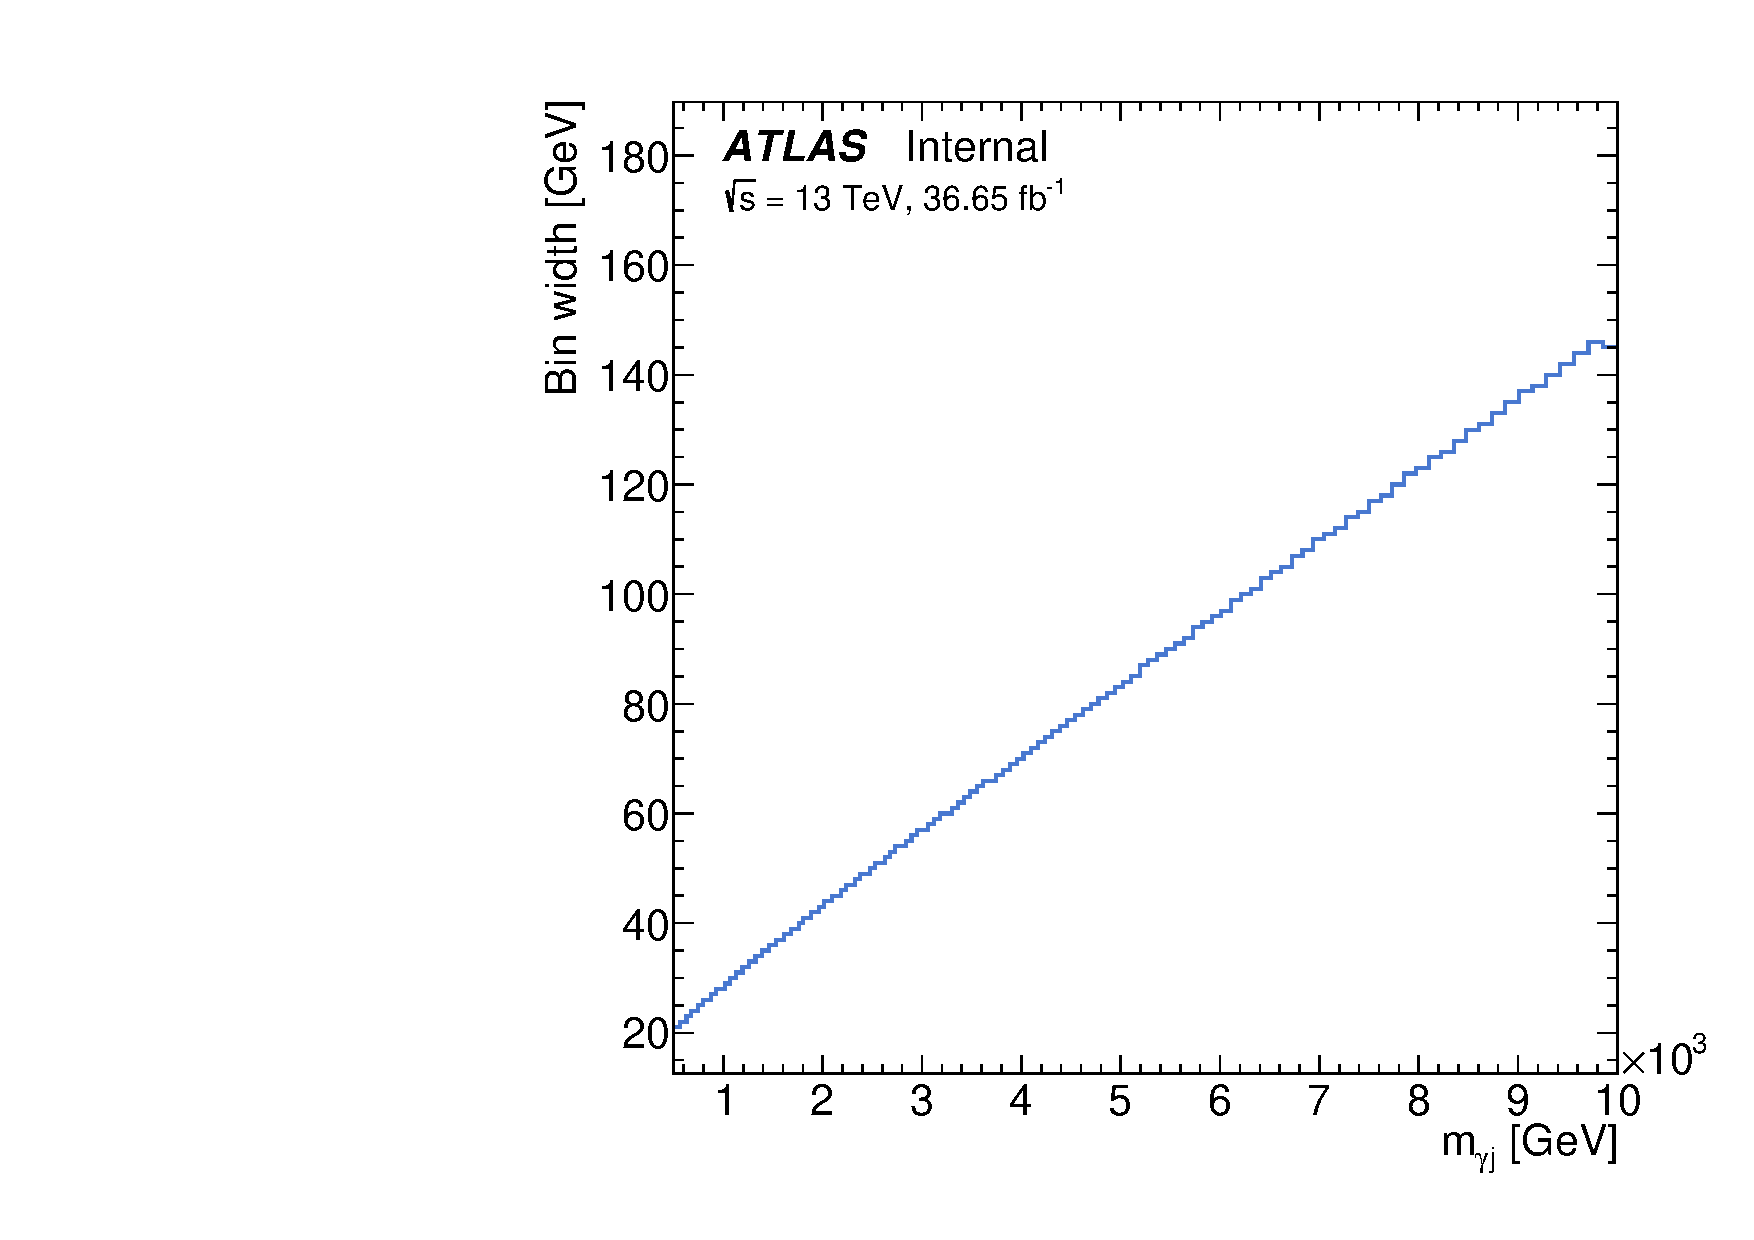
\includegraphics[width=\linewidth]{5_resonances/results/myj_binning/binning/can__SR__phjet_m_binwidth__2015_2016}
        \caption{Bin width as a function of \myj.}
        \label{fig:bkg_modeling:observable:results:binwidth}
    \end{subfigure}
    \hfill
    \begin{subfigure}[h]{0.49\linewidth}
        \centering
        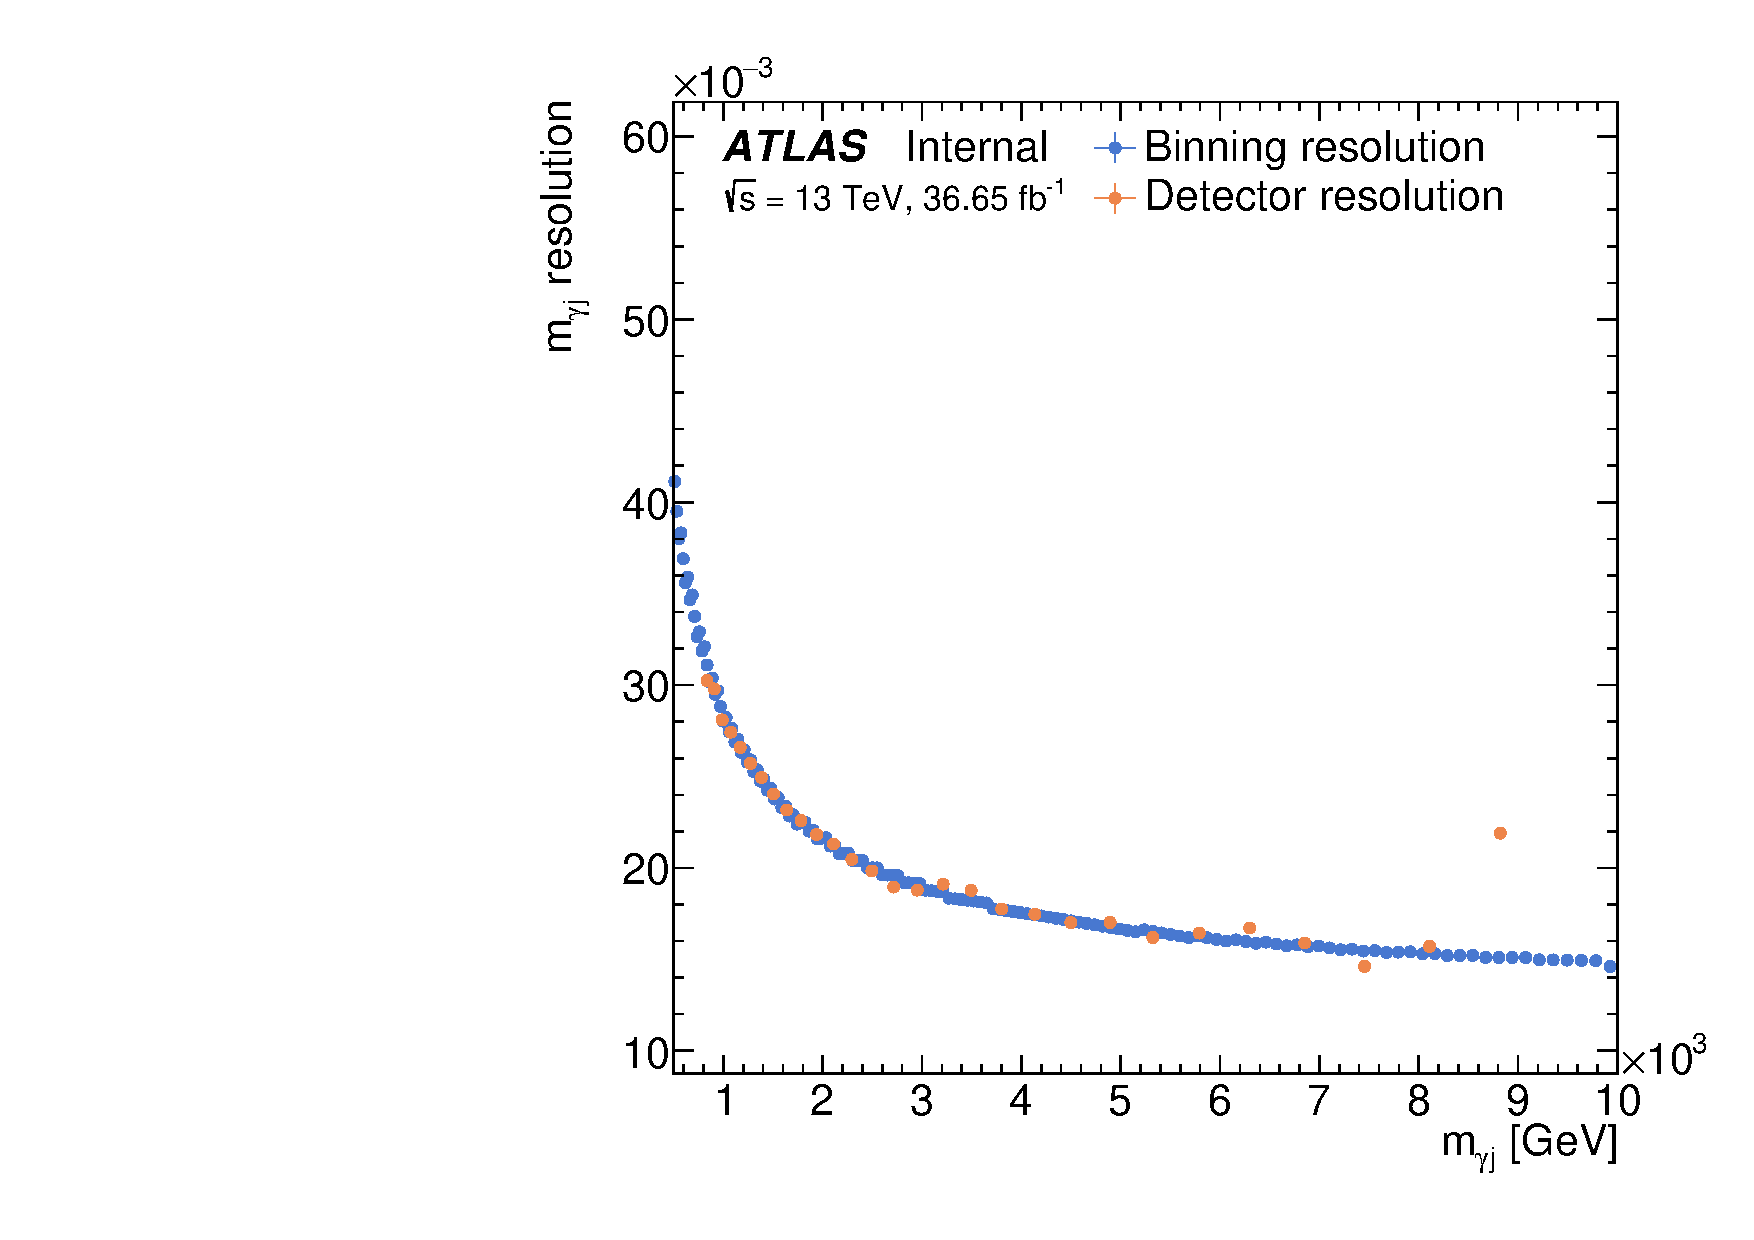
\includegraphics[width=\linewidth]{5_resonances/results/myj_binning/binning/can__SR__phjet_m_binresolution__2015_2016}
        \caption{Binning and detector resolution comparison.}
        \label{fig:bkg_modeling:observable:results:resolution_comparison}
    \end{subfigure}
    \caption{\myj binning optimisation results showing the bin-widths as a function of \myj (left) and the comparison between the binning resolution and detector resolution (right).}
    \label{fig:bkg_modeling:observable:results}
\end{figure}
%%%%%%%%%%%%%%%%%%%%%%%%%%%%%%%%%%%%%%%%%%%%%%%%%%%%%%%%%%%%%%%%%%%%%%%%%%%%%%%%%%%%%%%%%%%%%%%%%%%%
%%%%%%%%%%%%%%%%%%%%%%%%%%%%%%%%%%%%%%%%%%%%%%%%%%%%%%%%%%%%%%%%%%%%%%%%%%%%%%%%%%%%%%%%%%%%%%%%%%%%
%%%%%%%%%%%%%%%%%%%%%%%%%%%%%%%%%%%%%%%%%%%%%%%%%%%%%%%%%%%%%%%%%%%%%%%%%%%%%%%%%%%%%%%%%%%%%%%%%%%%
%%%%%%%%%%%%%%%%%%%%%%%%%%%%%%%%%%%%%%%%%%%%%%%%%%%%%%%%%%%%%%%%%%%%%%%%%%%%%%%%%%%%%%%%%%%%%%%%%%%%
%%%%%%%%%%%%%%%%%%%%%%%%%%%%%%%%%%%%%%%%%%%%%%%%%%%%%%%%%%%%%%%%%%%%%%%%%%%%%%%%%%%%%%%%%%%%%%%%%%%%
%%%%%%%%%%%%%%%%%%%%%%%%%%%%%%%%%%%%%%%%%%%%%%%%%%%%%%%%%%%%%%%%%%%%%%%%%%%%%%%%%%%%%%%%%%%%%%%%%%%%















%%%%%%%%%%%%%%%%%%%%%%%%%%%%%%%%%%%%%%%%%%%%%%%%%%%%%%%%%%%%%%%%%%%%%%%%%%%%%%%%%%%%%%%%%%%%%%%%%%%%
%%%%%%%%%%%%%%%%%%%%%%%%%%%%%%%%%%%%%%%%%%%%%%%%%%%%%%%%%%%%%%%%%%%%%%%%%%%%%%%%%%%%%%%%%%%%%%%%%%%%
%%%%%%%%%%%%%%%%%%%%%%%%%%%%%%%%%%%%%%%%%%%%%%%%%%%%%%%%%%%%%%%%%%%%%%%%%%%%%%%%%%%%%%%%%%%%%%%%%%%%
%%%%%%%%%%%%%%%%%%%%%%%%%%%%%%%%%%%%%%%%%%%%%%%%%%%%%%%%%%%%%%%%%%%%%%%%%%%%%%%%%%%%%%%%%%%%%%%%%%%%
%%%%%%%%%%%%%%%%%%%%%%%%%%%%%%%%%%%%%%%%%%%%%%%%%%%%%%%%%%%%%%%%%%%%%%%%%%%%%%%%%%%%%%%%%%%%%%%%%%%%
%%%%%%%%%%%%%%%%%%%%%%%%%%%%%%%%%%%%%%%%%%%%%%%%%%%%%%%%%%%%%%%%%%%%%%%%%%%%%%%%%%%%%%%%%%%%%%%%%%%%
\section{Results}
\label{sec:results:results}

Now that the fitting strategies are defined for each one of the signal regions and signal models considered (see \Tab{\ref{tab:bkg:modeling:strategy_modeling:summary}}), the fits are now applied to the observed \myj in data. Two different types of interpretations are studied:
\begin{itemize}
    \item \textbf{\acf{BO} interpretation}: A \ac{BO} fit is performed to data in each one of the signal regions, in order to test the compatibility of the data with a smoothly falling spectrum. In case any excess is found, it is quantified by virtue of the \bh algorithm previously discussed.
    \item \textbf{Signal interpretation}: The compatibility of the data with three different signal models is studied. One of the models correspond to generic Gaussian shapes, which allow to interpret the results in a more general way. The other two benchmark models correspond to \acp{QBH} and \acp{EQ} models, where their resonance shapes are different between them, and also for different parameters of the theories. In case no significant excess is found with the \ac{BO} interpretation, exclusion limits on the parameter values of these theories are derived.
\end{itemize}




%%%%%%%%%%%%%%%%%%%%%%%%%%%%%%%%%%%%%%%%%%%%%%%%%%%%%%%%%%%%%%%%%%%%%%%%%%%%%%%%%%%%%%%%%%%%%%%%%%%%
%%%%%%%%%%%%%%%%%%%%%%%%%%%%%%%%%%%%%%%%%%%%%%%%%%%%%%%%%%%%%%%%%%%%%%%%%%%%%%%%%%%%%%%%%%%%%%%%%%%%
%%%%%%%%%%%%%%%%%%%%%%%%%%%%%%%%%%%%%%%%%%%%%%%%%%%%%%%%%%%%%%%%%%%%%%%%%%%%%%%%%%%%%%%%%%%%%%%%%%%%
\subsection{Background-only interpretation}
\label{subsec:results:results:bkgonly}

The fit strategies derived in the previous chapter are now applied to the observed \myj distribution in data. This allows to perform an interpretation of the invariant mass distribution without any assumption on the potential signal other than it being a localised effect. However, the consistency of the observed \gammajet mass spectrum with a smoothly falling \ac{SM} background can not be quantified with the \(p(\chisq)\)-value alone. This, does not provide the optimal sensitivity to a localized resonance since it considers all \myj bins simultaneously and independently of each other. A true resonance, on the other hand, would likely result in a correlated excess in one or several adjacent \myj bins, and here is when the \bh algorithm comes to place.

\begin{figure}[ht!]
    \centering
    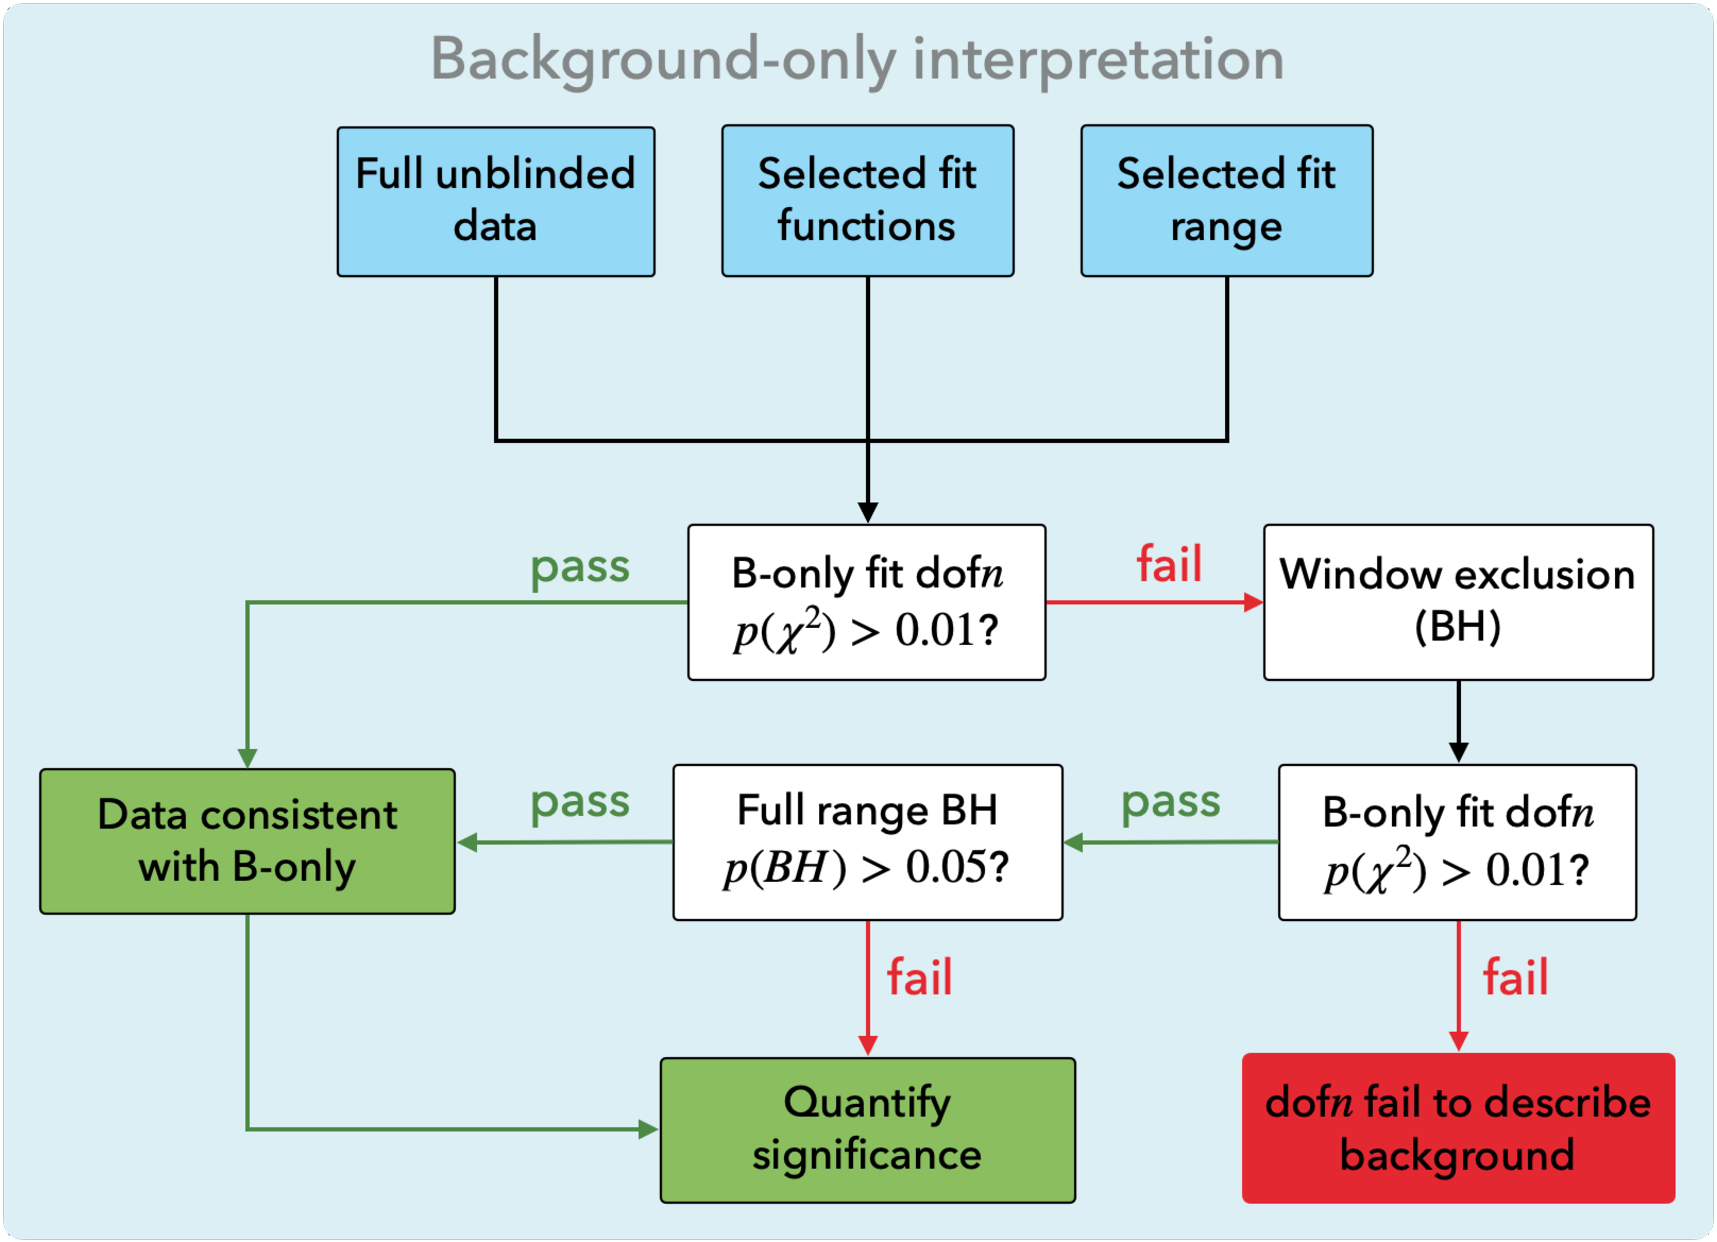
\includegraphics[width=0.7\linewidth]{5_resonances/results/bkgonly/unblind_strategy3_bo}
    \caption{Scheme of the \ac{BO} fit worflow to data.}
    \label{fig:results:results:bkgonly:strat}
\end{figure}

The \ac{BO} fit workflow is shown in \Fig{\ref{fig:results:results:bkgonly:strat}}. For each signal region, the first step is to perform a \ac{BO} fit to observed \myj spectrum. If the \chisq \pval of this fit exceeds a threshold of 0.01, the \ac{BO} hypothesis succeeds to describe the data and \bh is run to identify the most significant deviation and assign a \pval to it. On the other hand, if the \(p(\chisq)\)-threshold is not passed, that can either hint at the fit not being able to globally describe the data spectrum or at one or more localized deviations. In order to test the latter case, \bh is executed to identify the most significant deviation. This region is subsequently masked and the \ac{BO} fit is repeated and the \(p(\chisq)\)-value is checked again. If it does not pass the threshold, a single local effect cannot explain the bad fit and no clear interpretation of the observed spectrum can be given. If on the other hand the threshold is passed, this means that indeed the local effect was preventing a good fit. The \bh is run again and a \pval is assigned to this most significant deviation. A \pval larger than 0.05 is then interpreted as no significant \bh discovery. If on the other hand this threshold is not exceeded, a local effect is assumed and the significance of hypothetical signal is evaluated.

\subsubsection{Results}

\begin{figure}[ht!]
    \centering
    \begin{subfigure}[h]{0.49\linewidth}
        \centering
        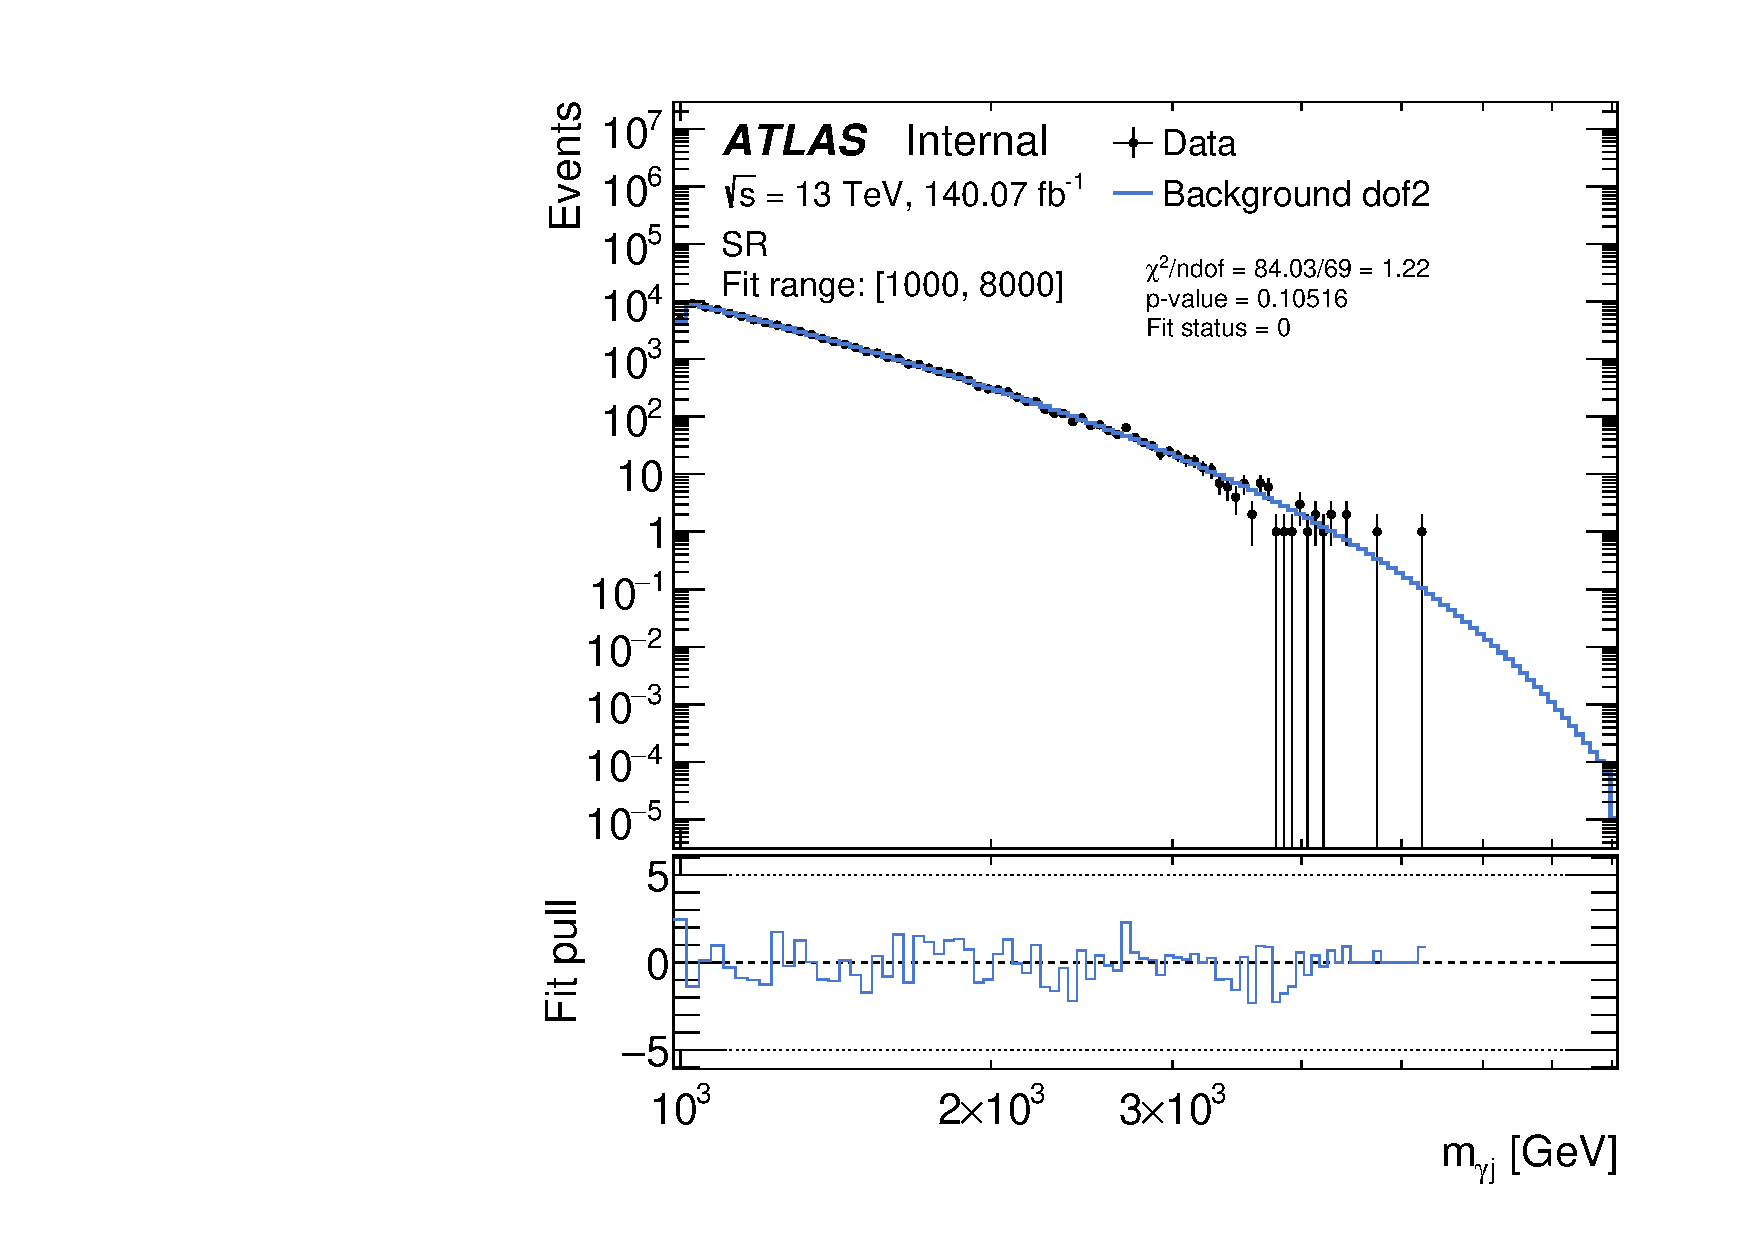
\includegraphics[width=\linewidth]{5_resonances/results/bkgonly/SR/dof2__range_1000_8000/plots/can__bkgonlyfit__asimov__data__SR__dof2__range_1000_8000}
        \caption{SR}
        \label{fig:results:results:bkgonly:fits:SR}
    \end{subfigure}
    \hfill
    \begin{subfigure}[h]{0.49\linewidth}
        \centering
        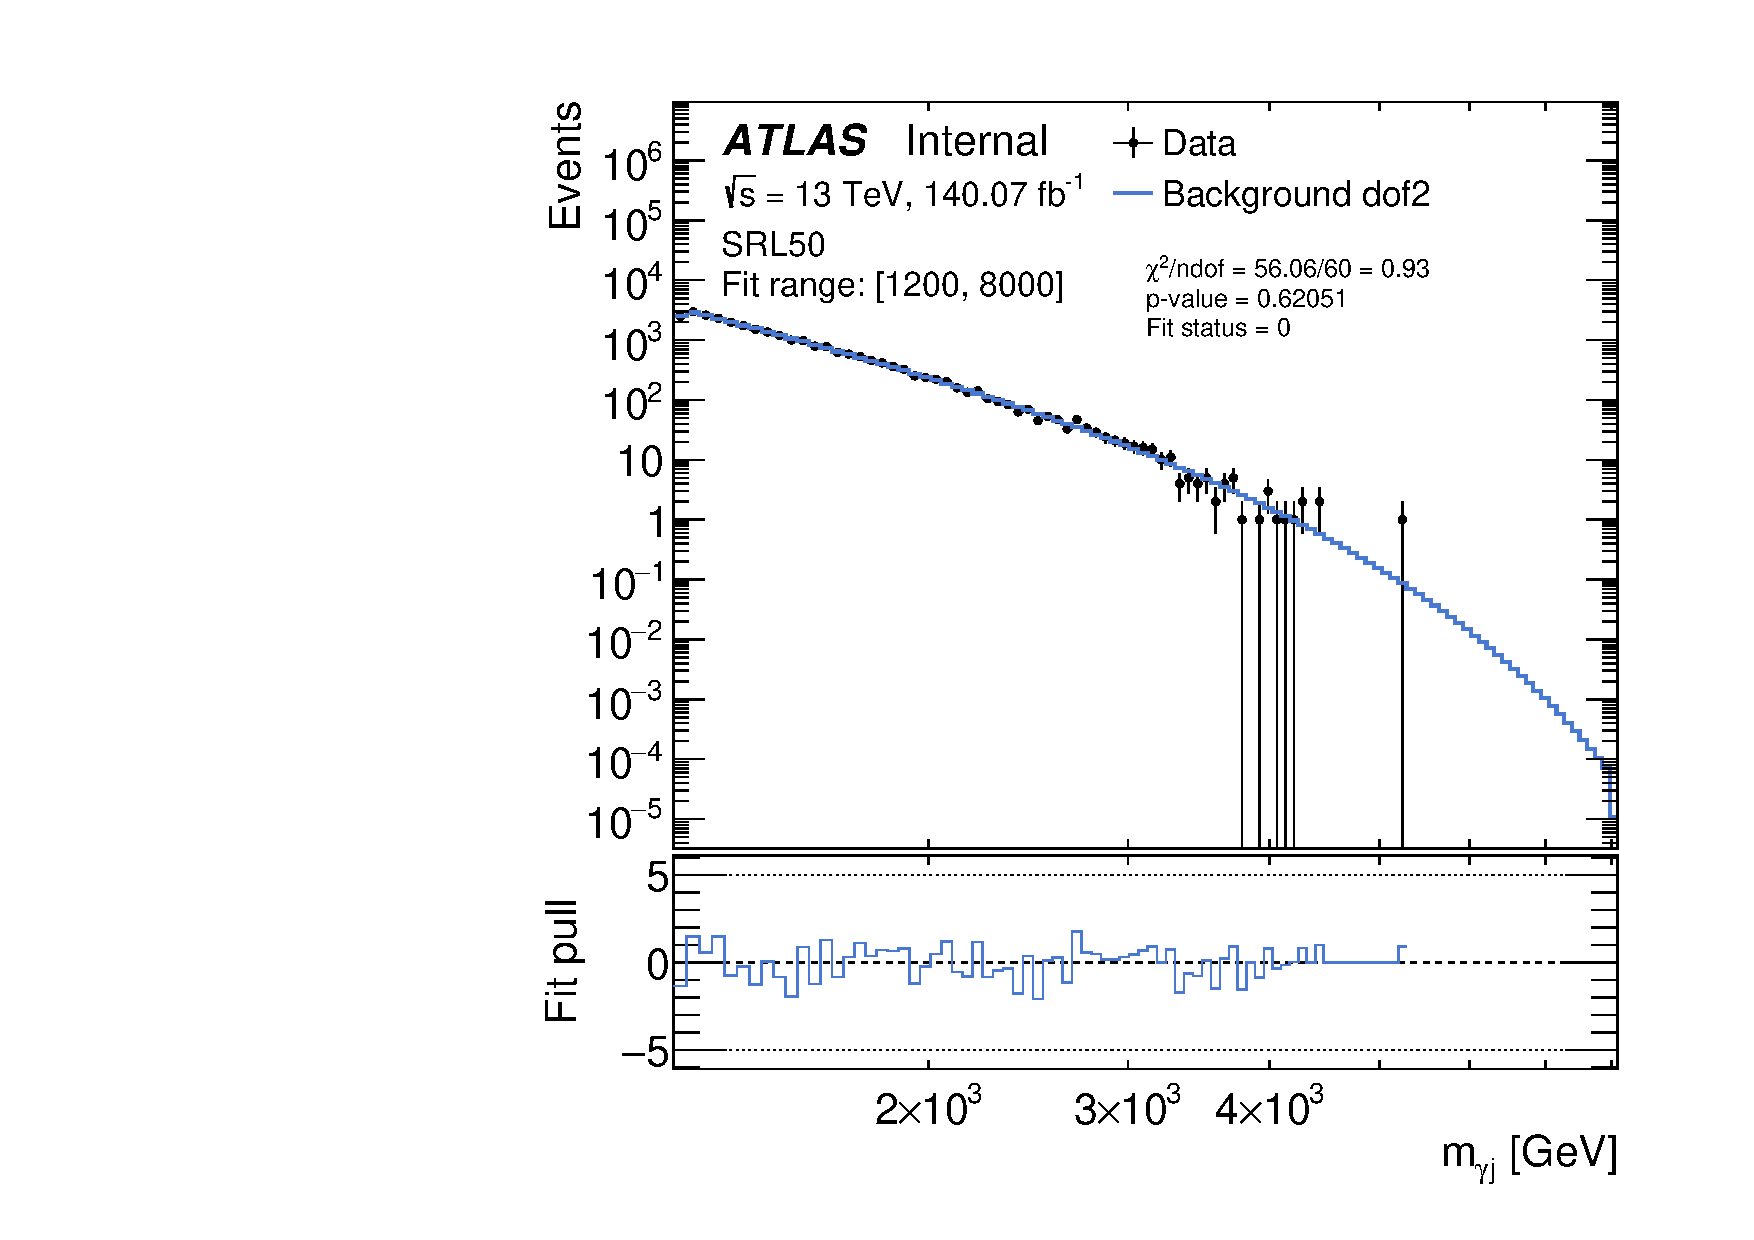
\includegraphics[width=\linewidth]{5_resonances/results/bkgonly/SRL50/dof2__range_1200_8000/plots/can__bkgonlyfit__asimov__data__SRL50__dof2__range_1200_8000}
        \caption{SRL}
        \label{fig:results:results:bkgonly:fits:SRL50}
    \end{subfigure}\\
    \begin{subfigure}[h]{0.49\linewidth}
        \centering
        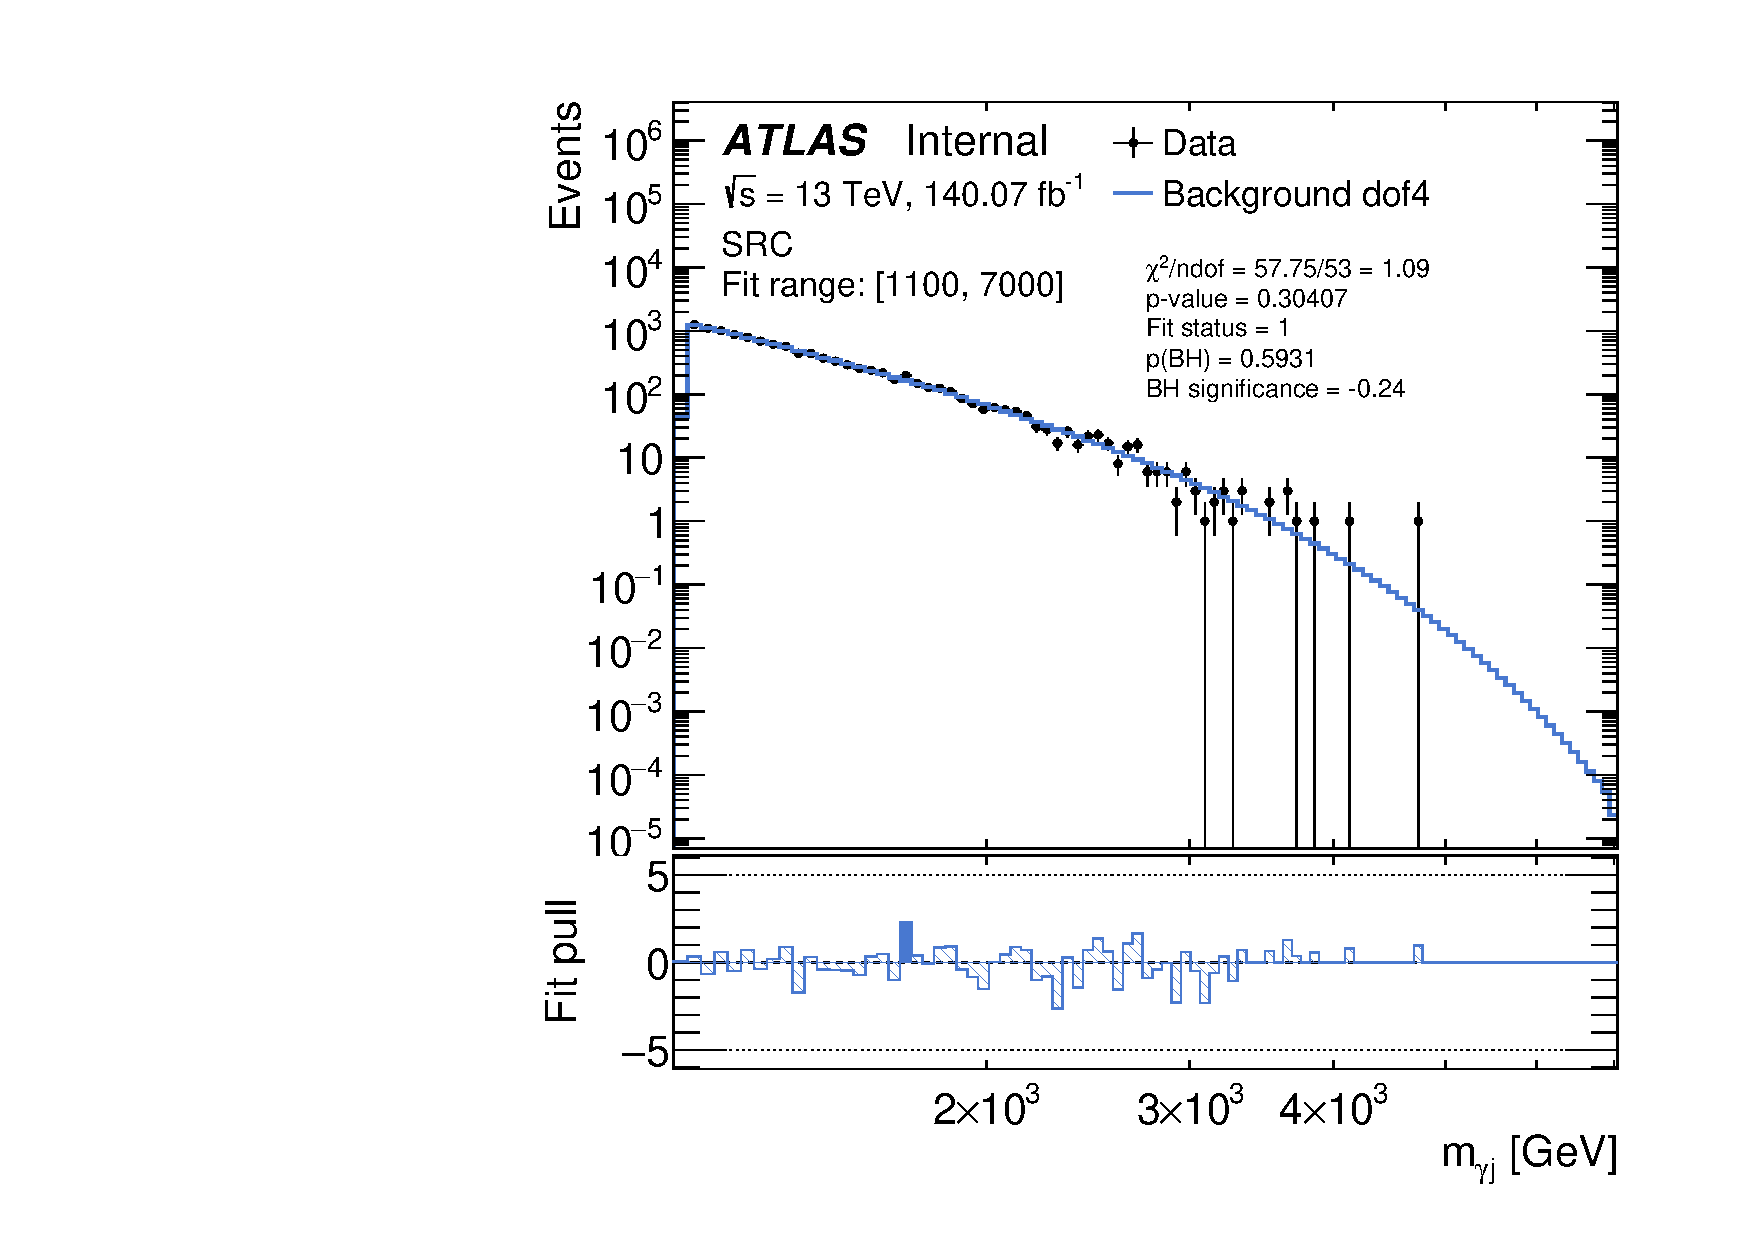
\includegraphics[width=\linewidth]{5_resonances/results/bkgonly/SRC50/dof4__range_1100_7000/plots/can__bkgonlyfit__asimov__data__SRC50__dof4__range_1100_7000}
        \caption{SRC}
        \label{fig:results:results:bkgonly:fits:SRC}
    \end{subfigure}
    \hfill
    \begin{subfigure}[h]{0.49\linewidth}
        \centering
        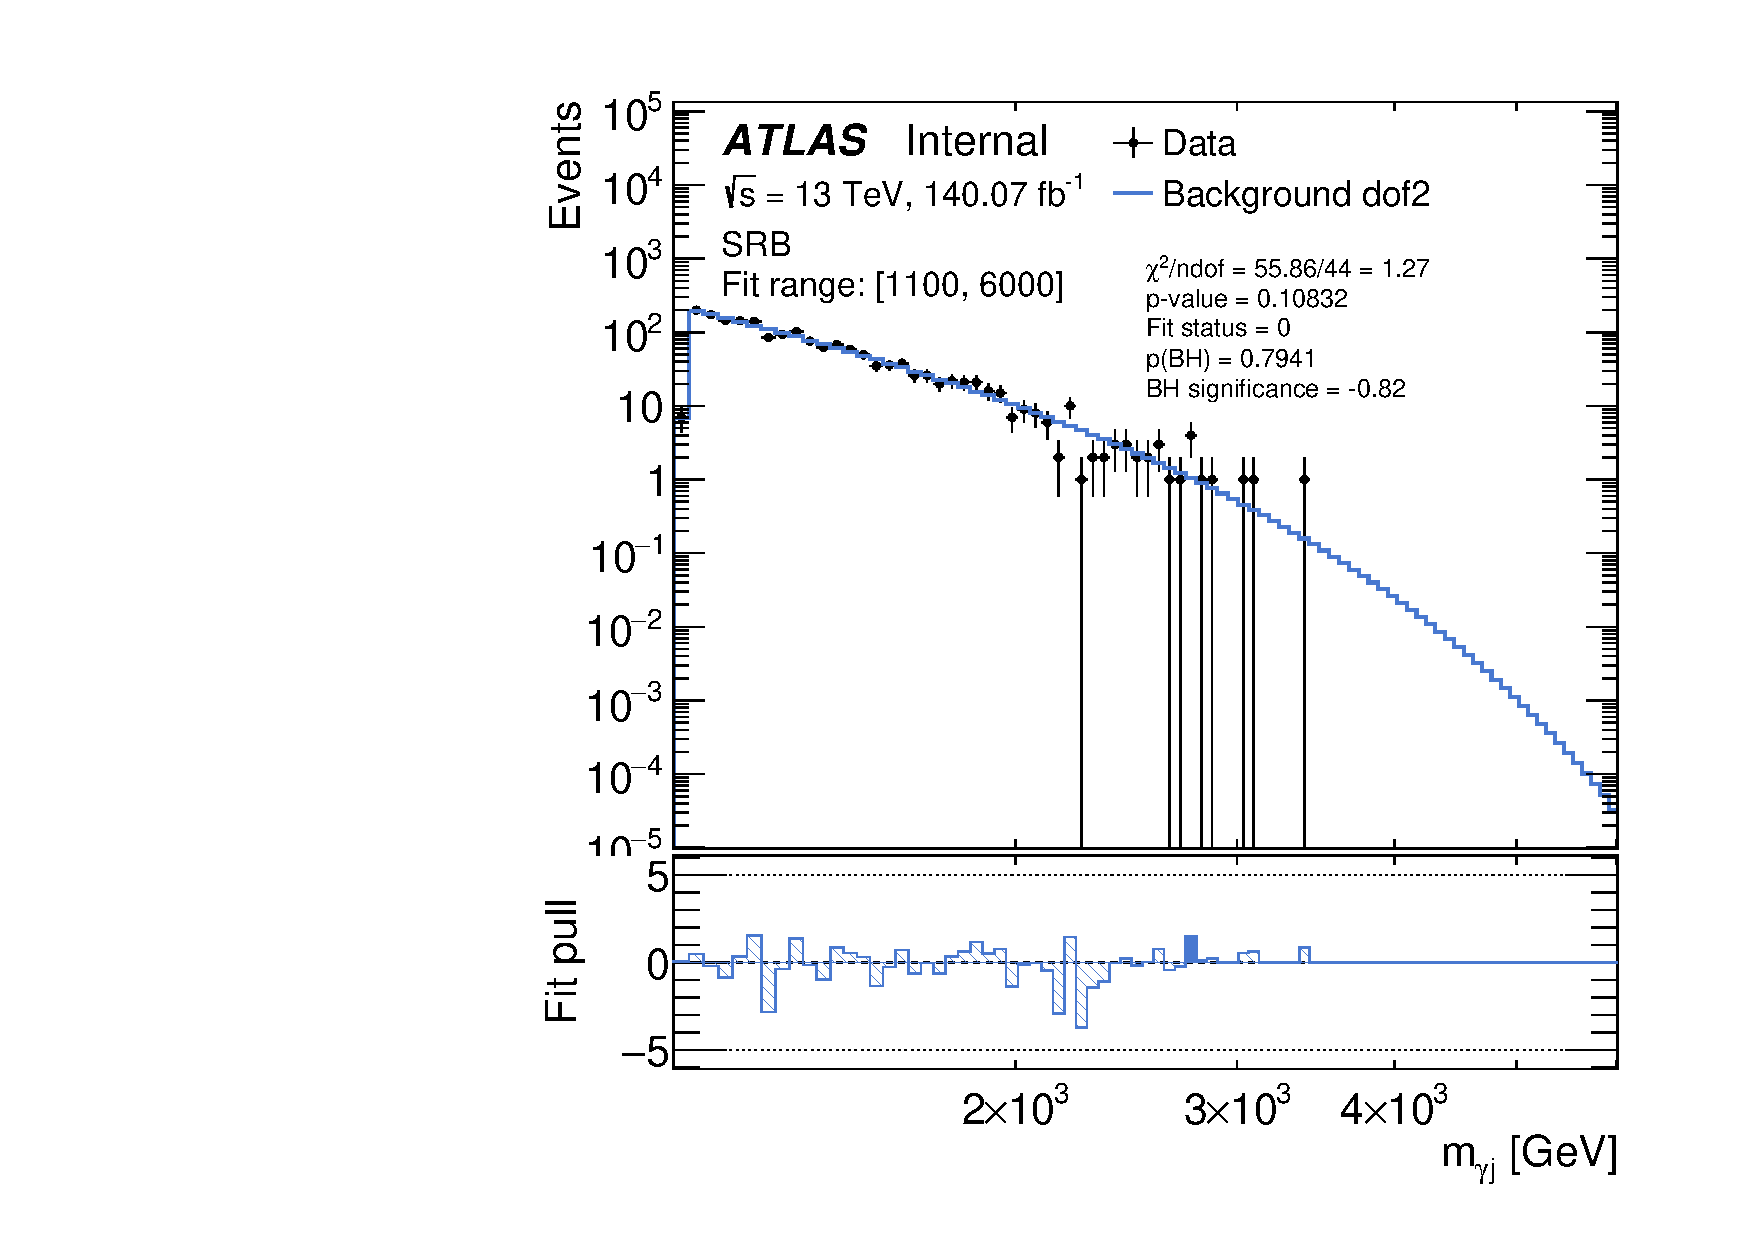
\includegraphics[width=\linewidth]{5_resonances/results/bkgonly/SRB/dof2__range_1100_6000/plots/can__bkgonlyfit__asimov__data__SRB__dof2__range_1100_6000}
        \caption{SRB}
        \label{fig:results:results:bkgonly:fits:SRB}
    \end{subfigure}
    \caption{\ac{BO} fits to full Run-2 data in the four considered analysis regions. The data distribution and the background fit are shown in the top pad, while the normalised residues (or pull) in the lower pad. Moreover, fit \chisq and \pval are displayed for each region.}
    \label{fig:results:results:bkgonly:fits}
\end{figure}

The resulting fits in each signal region are shown in \Fig{\ref{fig:results:results:bkgonly:fits}}. It can be seen that no significant excess is found in neither of the regions. The lower pad of each one of the figures shows the normalised residues of the fit, where differences between data and the \ac{BO} hypothesis can be more easily identified. The major differences observed between the background estimate and the actual data are downward data fluctuations, specially seen for the SRB region at \(\sim 2100~\gev\). These type of downwards fluctuations make the quality of the fit to decrease, but not drastically.
Although there are bins in which the difference is close to a \(+2\sigma\) deviation, these deviations are better identified by the \bh algorithm in the following.

Considering that the \(p(\chisq)\)-values in the \ac{BO} fits did not present any sign of deviation from the \ac{BO} hypothesis, that is, no significant difference between the background model and the data, the dedicated \bh algorithm is run to identify where the most significant deviation is. Moreover, the deviation is quantified in terms of the \bh \pval, calculated as indicated by \Eqn{\ref{eq:strategy:stat_treatment:bh:bh_pval}}.
These results are shown in \Figrange{\ref{fig:results:results:bkgonly:bh:SR}}{\ref{fig:results:results:bkgonly:bh:SRB}}, where the most significant bump is marked with the red dashed lines in the \myj spectrum, obtained where the local \pval is found to be maximum, as indicated by the figures on the right-hand side for each case. In all cases, the global \(p(\text{BH})\) and significance is indicated in the caption.

\begin{figure}[ht!]
    \centering
    \begin{subfigure}[h]{0.49\linewidth}
        \centering
        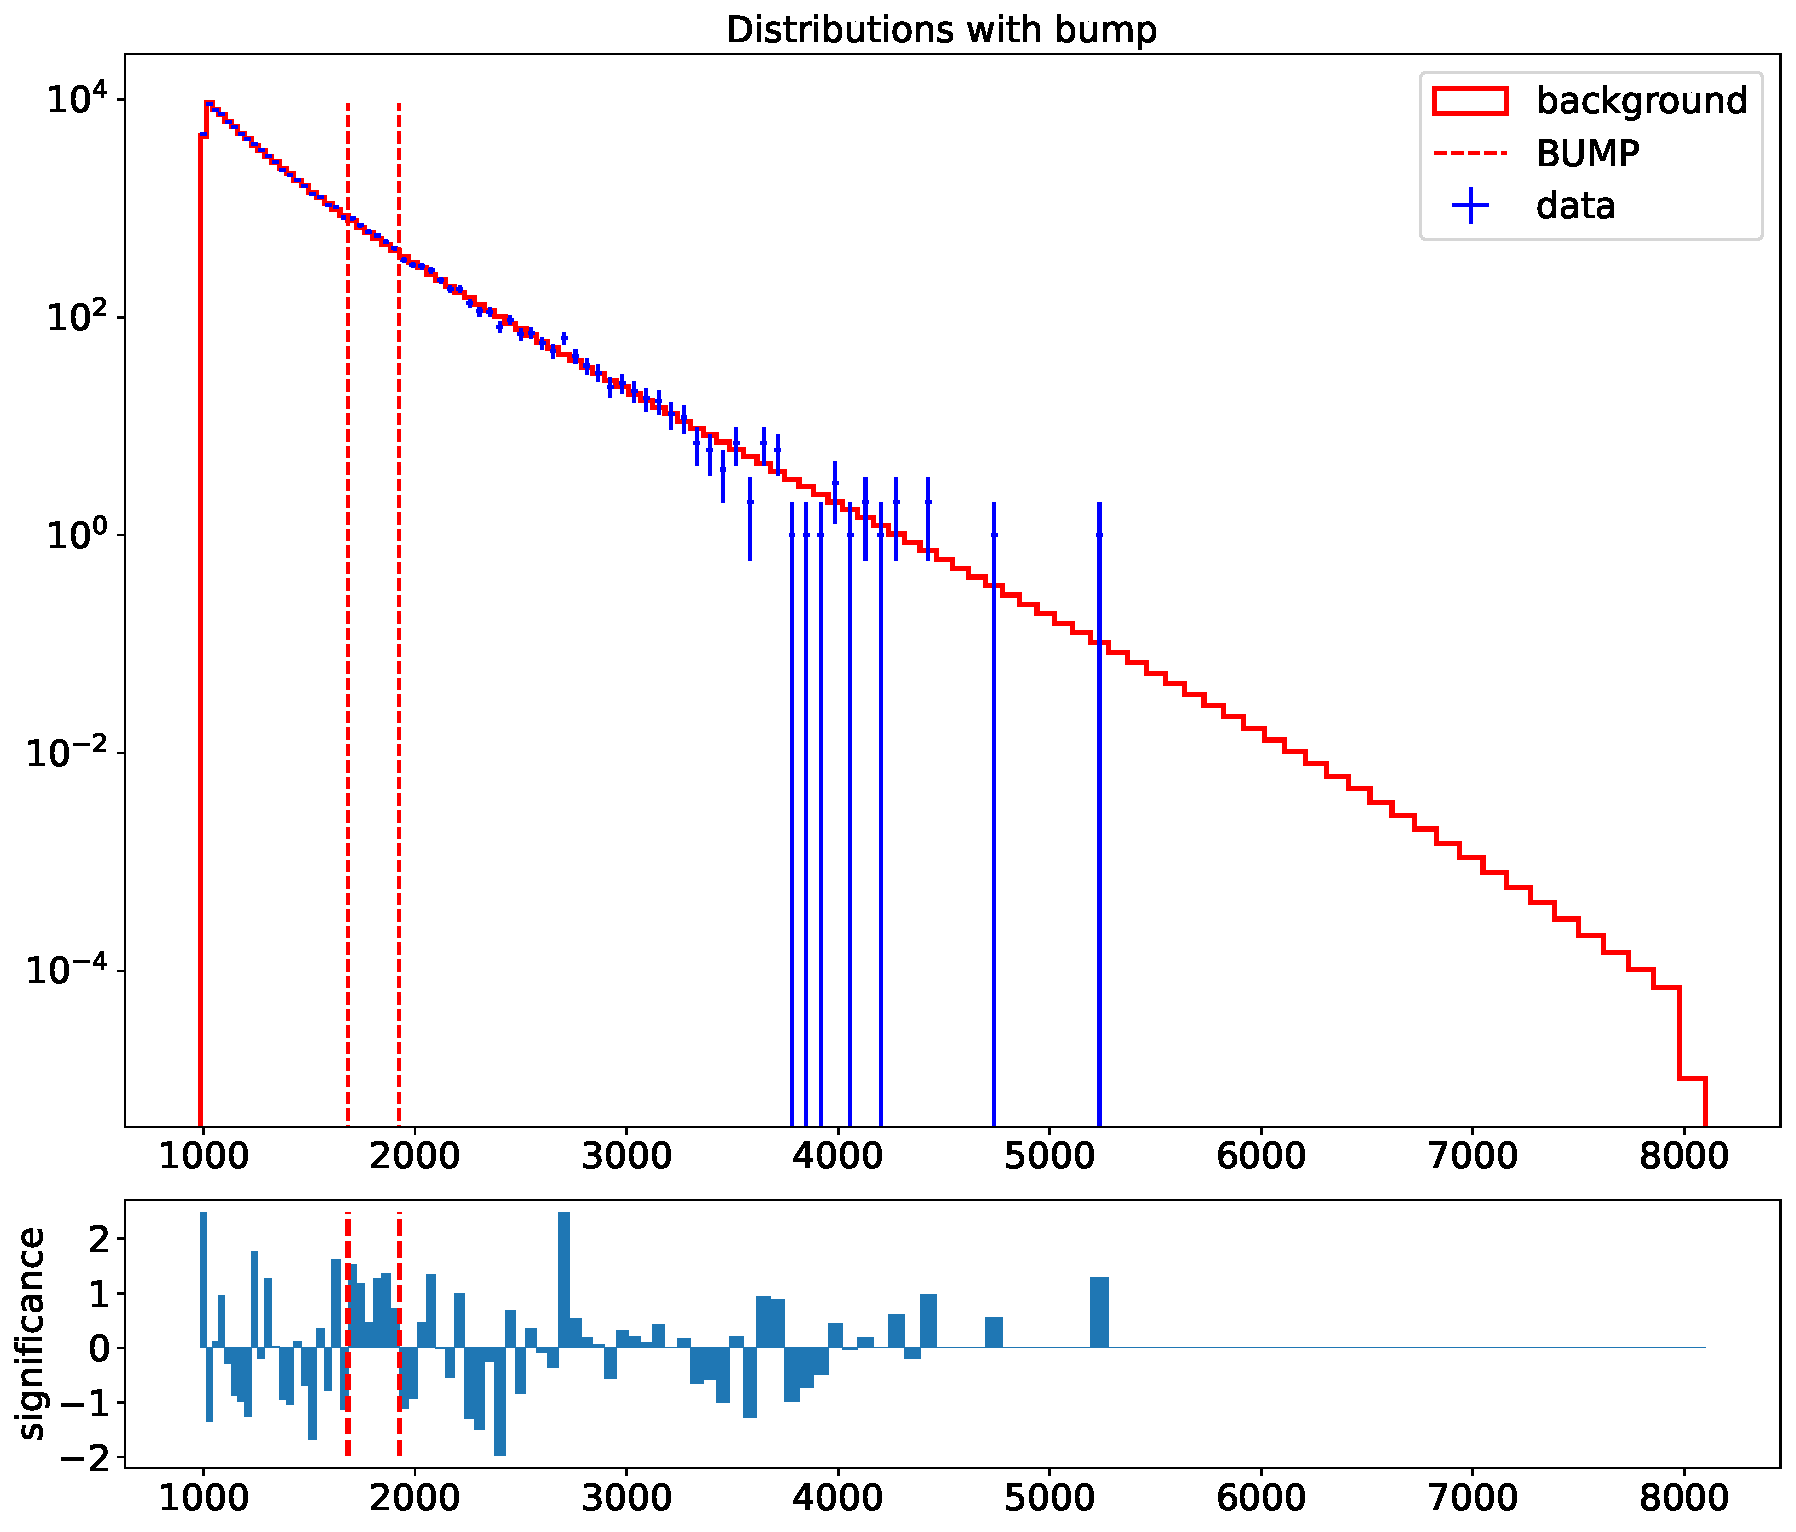
\includegraphics[width=\linewidth]{5_resonances/results/bkgonly/SR/dof2__range_1000_8000/fits/BHoutput__dof2__data__SR__asimov_bump}
        \caption{Most significant bump.}
    \end{subfigure}
    \hfill
    \begin{subfigure}[h]{0.49\linewidth}
        \centering
        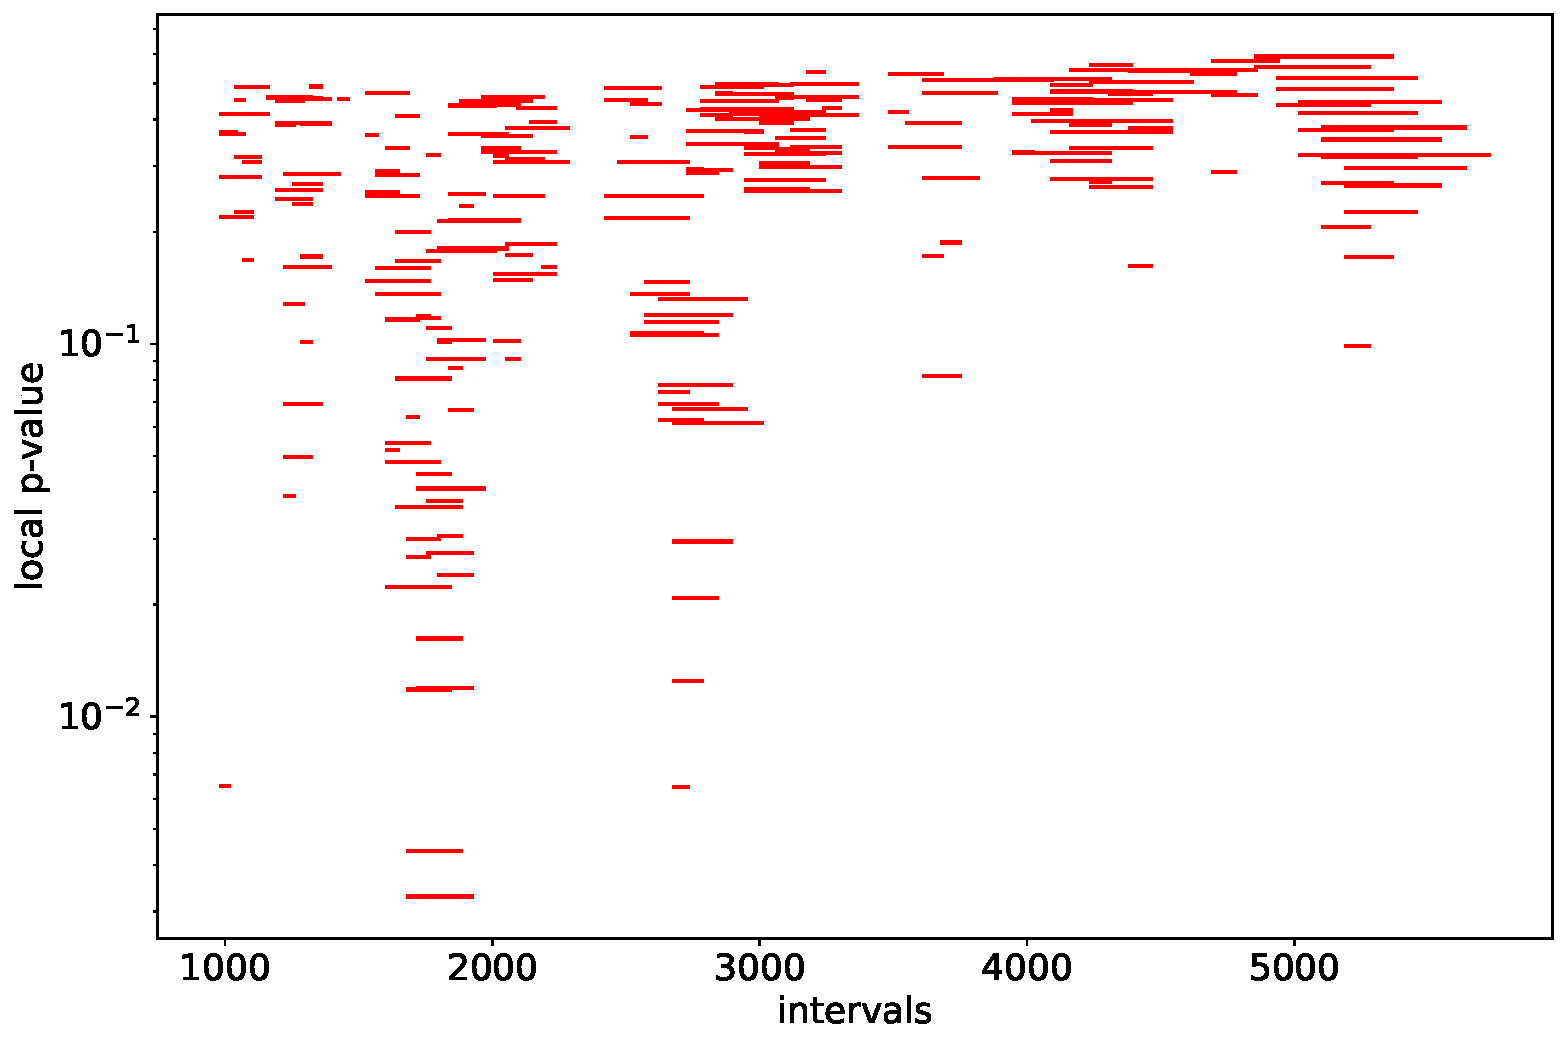
\includegraphics[width=\linewidth]{5_resonances/results/bkgonly/SR/dof2__range_1000_8000/fits/BHoutput__dof2__data__SR__asimov_tompgraphy}
        \caption{Tomography scan showing Local \pval.}
    \end{subfigure}
    \caption{\bh results for region SR. The figure on the left shows the most significant bump, marked with red dashed lines. On the right, the local \pval for different tested windows is presented, indicating where the most significant excess is located. The global \(p(\text{BH})\) as calculated by \Eqn{\ref{eq:strategy:stat_treatment:bh:bh_pval}} is \(0.3938\), while the global significance \(-0.009\).}
    \label{fig:results:results:bkgonly:bh:SR}
\end{figure}

\begin{figure}[ht!]
    \centering
    \begin{subfigure}[h]{0.49\linewidth}
        \centering
        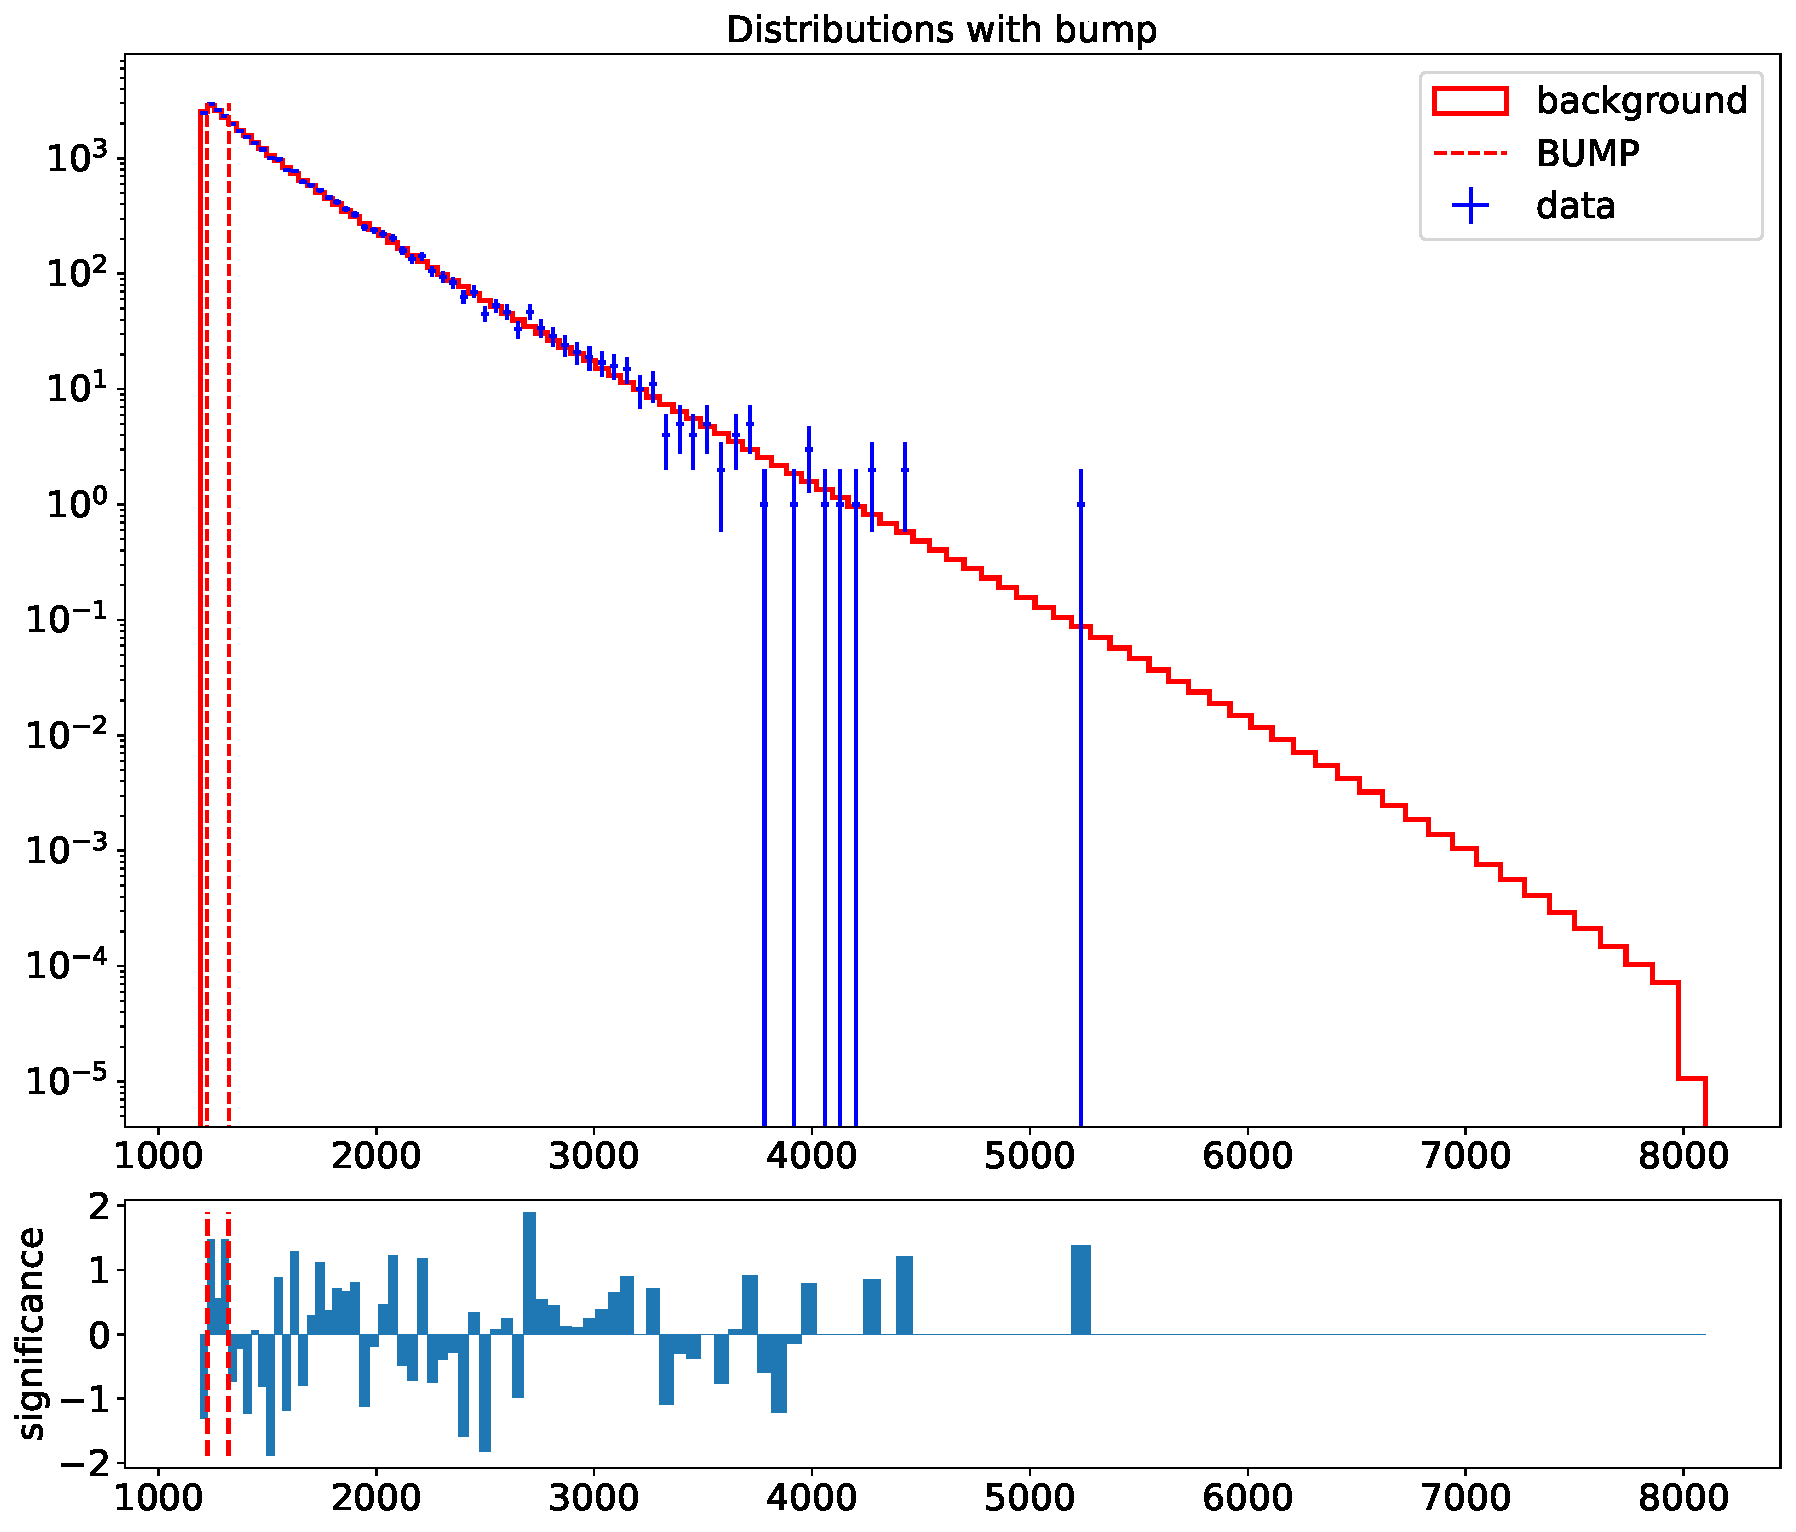
\includegraphics[width=\linewidth]{5_resonances/results/bkgonly/SRL50/dof2__range_1200_8000/fits/BHoutput__dof2__data__SRL50__asimov_bump}
        \caption{Most significant bump.}
    \end{subfigure}
    \hfill
    \begin{subfigure}[h]{0.49\linewidth}
        \centering
        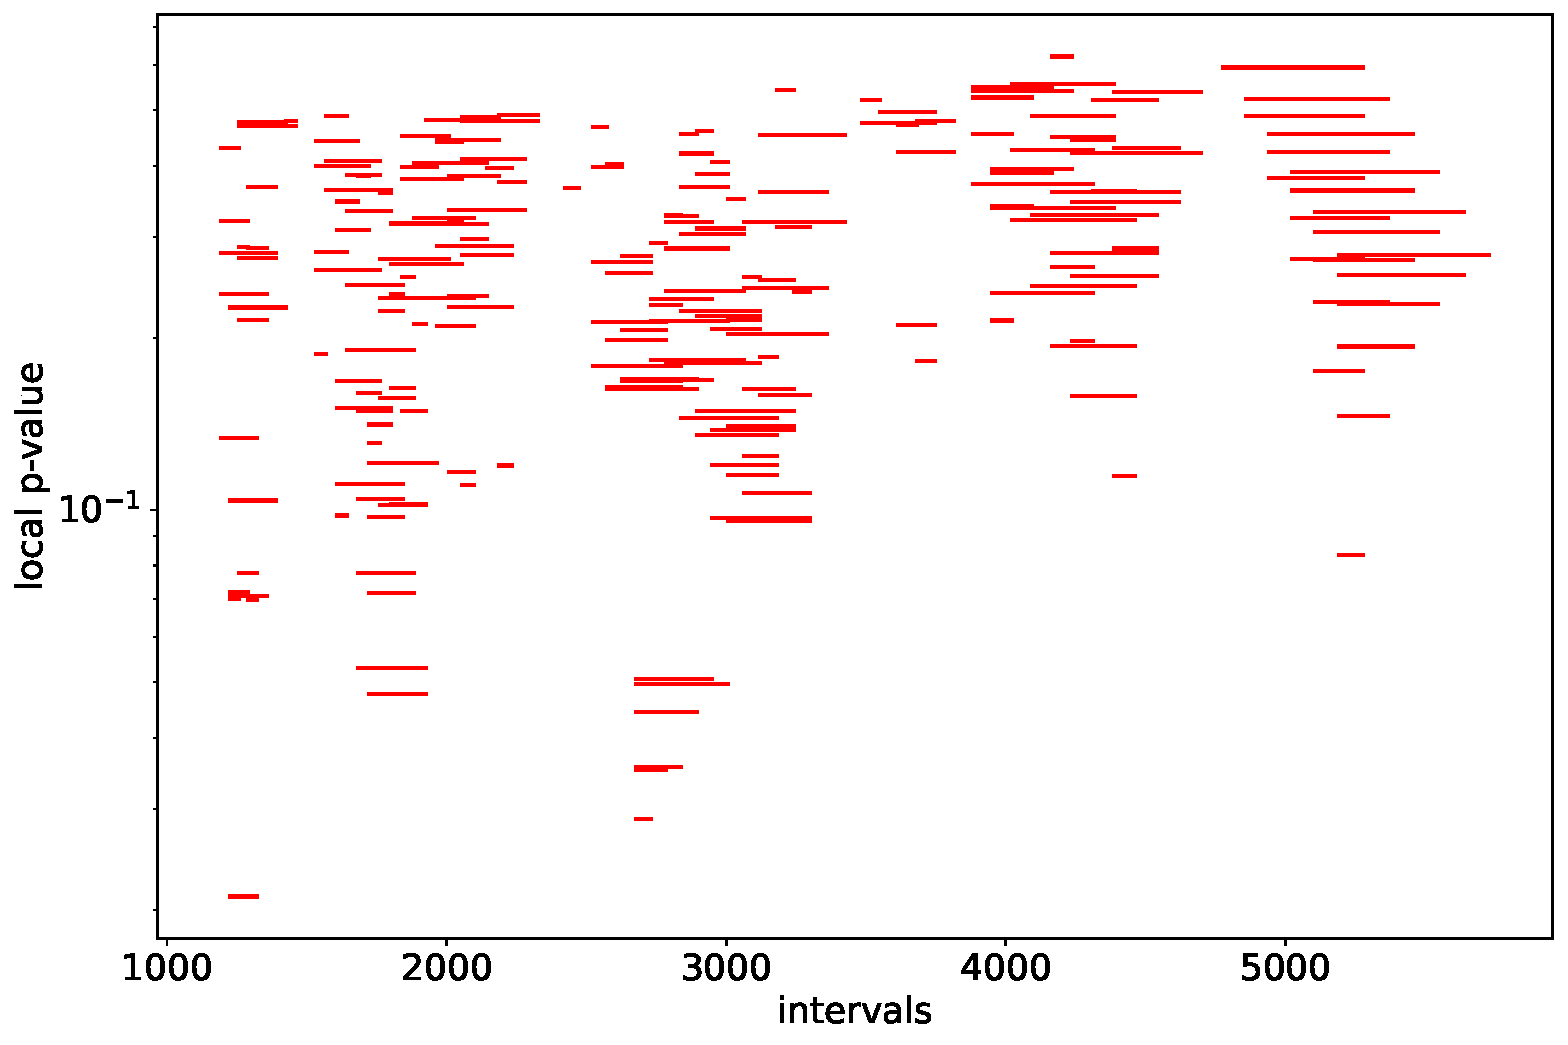
\includegraphics[width=\linewidth]{5_resonances/results/bkgonly/SRL50/dof2__range_1200_8000/fits/BHoutput__dof2__data__SRL50__asimov_tompgraphy}
        \caption{Tomography scan showing Local \pval.}
    \end{subfigure}
    \caption{Same as \Fig{\ref{fig:results:results:bkgonly:bh:SR}} but in region SRL, where the resulting global \(p(\text{BH}) = 0.8790\) and significance \(-1.170\).}
    \label{fig:results:results:bkgonly:bh:SRL}
\end{figure}

\begin{figure}[ht!]
    \centering
    \begin{subfigure}[h]{0.49\linewidth}
        \centering
        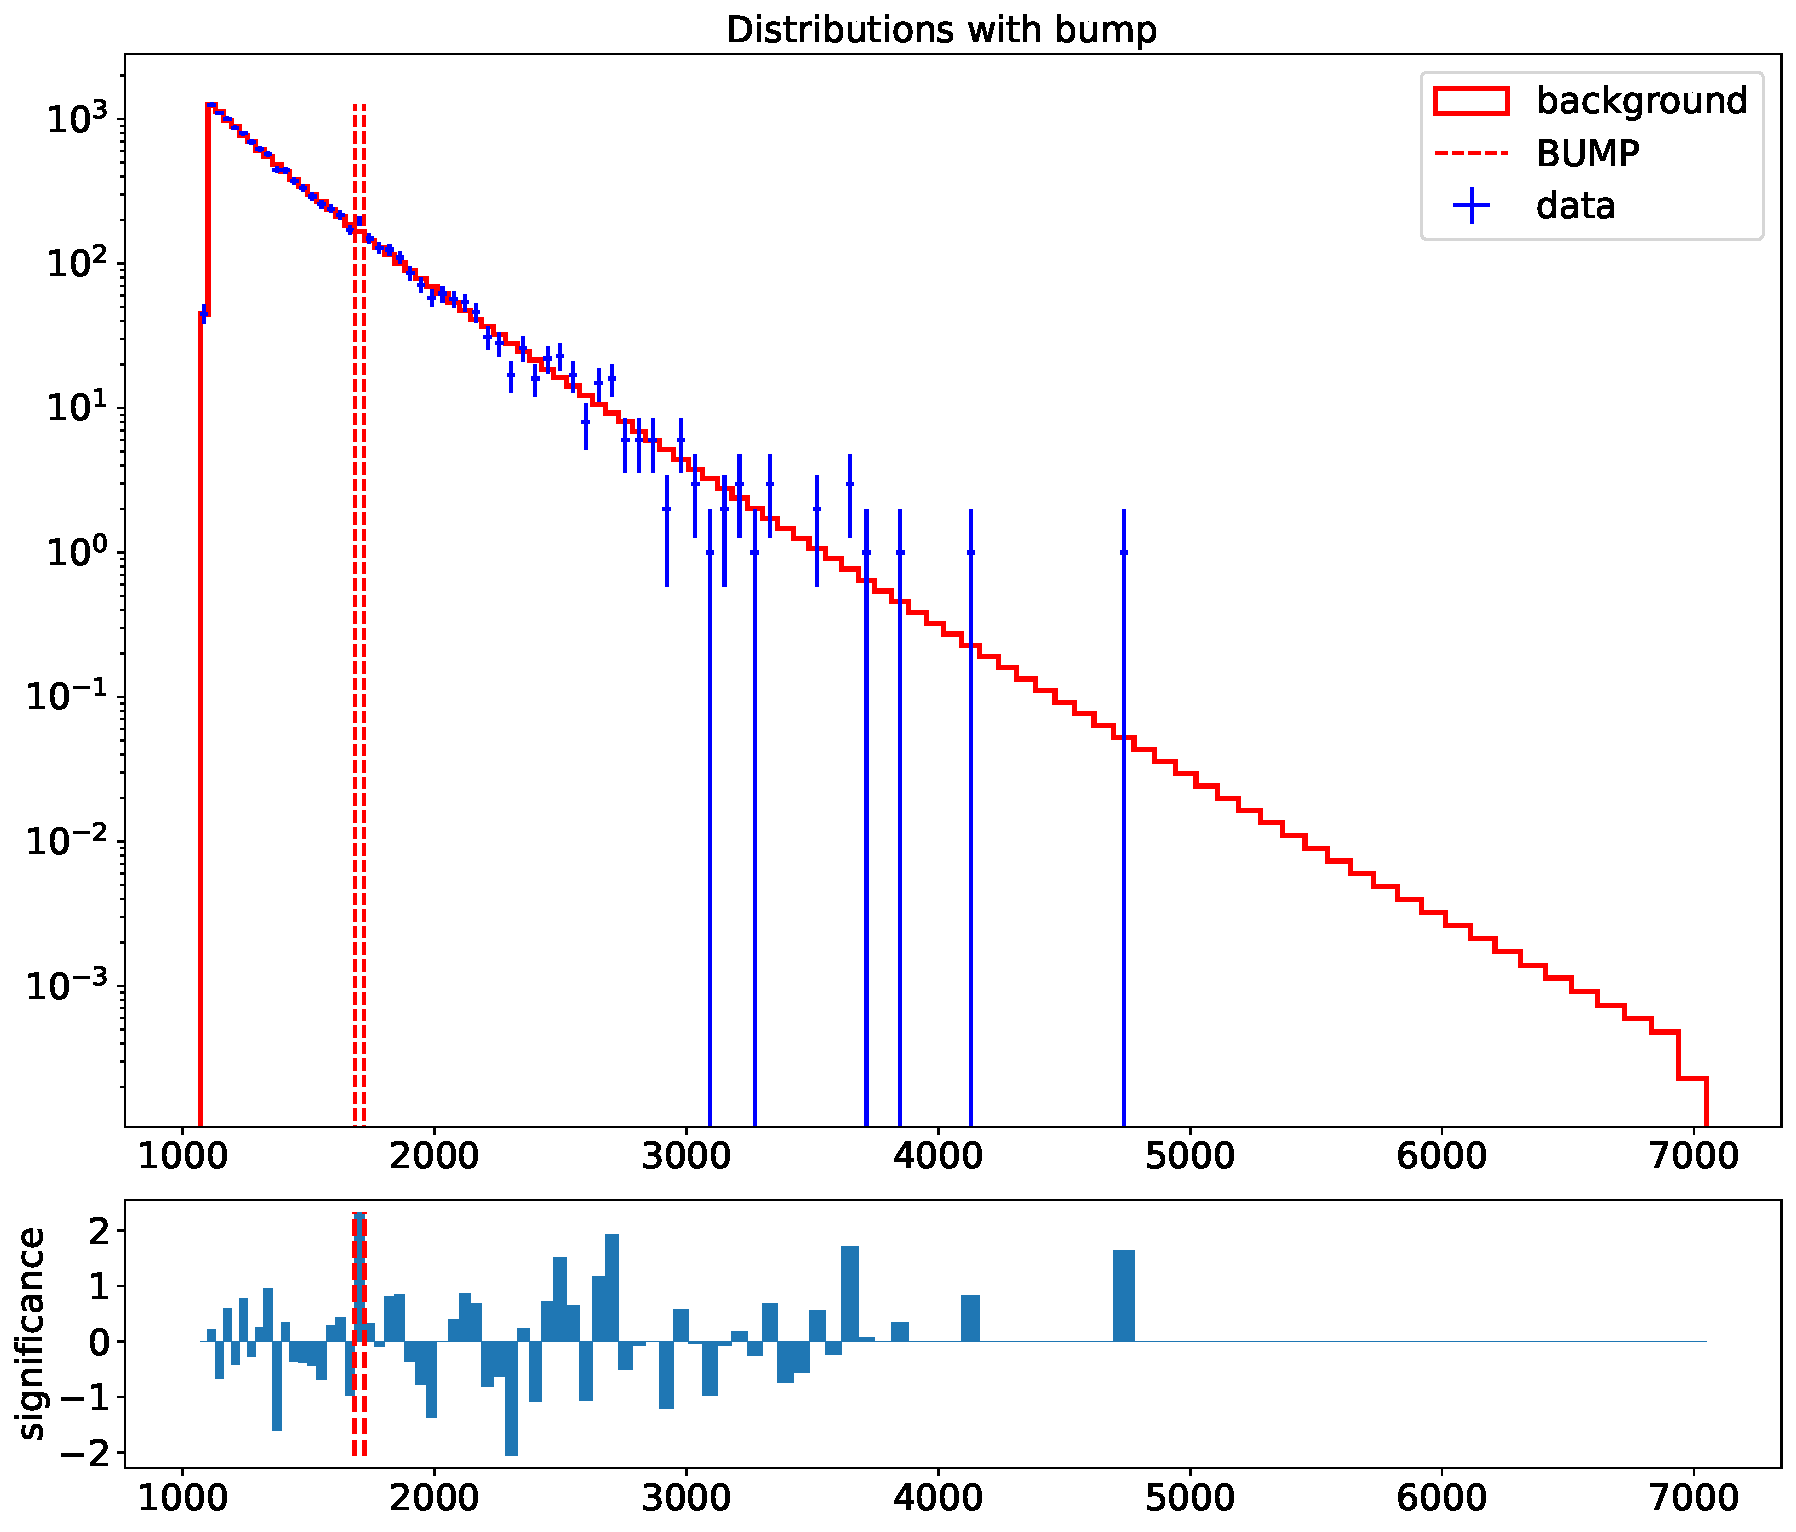
\includegraphics[width=\linewidth]{5_resonances/results/bkgonly/SRC50/dof4__range_1100_7000/fits/BHoutput__dof4__data__SRC50__asimov_bump}
        \caption{Most significant bump.}
    \end{subfigure}
    \hfill
    \begin{subfigure}[h]{0.49\linewidth}
        \centering
        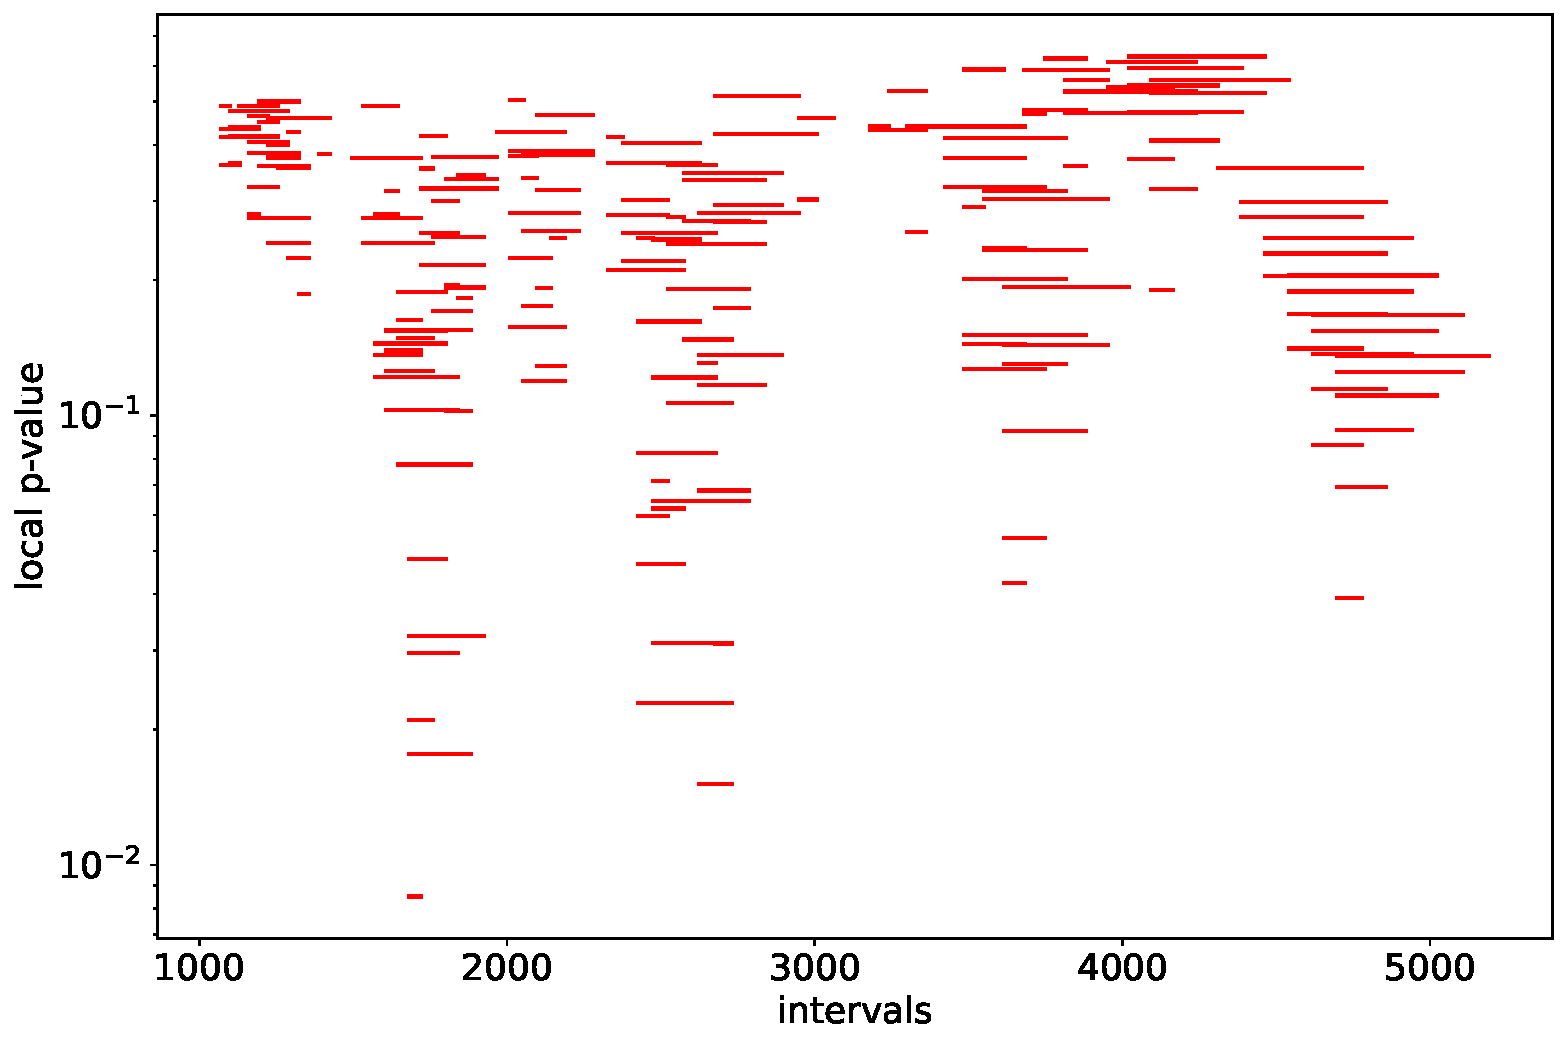
\includegraphics[width=\linewidth]{5_resonances/results/bkgonly/SRC50/dof4__range_1100_7000/fits/BHoutput__dof4__data__SRC50__asimov_tompgraphy}
        \caption{Tomography scan showing Local \pval.}
    \end{subfigure}
    \caption{Same as \Fig{\ref{fig:results:results:bkgonly:bh:SR}} but in region SRC, where the resulting global \(p(\text{BH}) = 0.6438\) and significance \(-0.368\).}
    \label{fig:results:results:bkgonly:bh:SRC}
\end{figure}

\begin{figure}[ht!]
    \centering
    \begin{subfigure}[h]{0.49\linewidth}
        \centering
        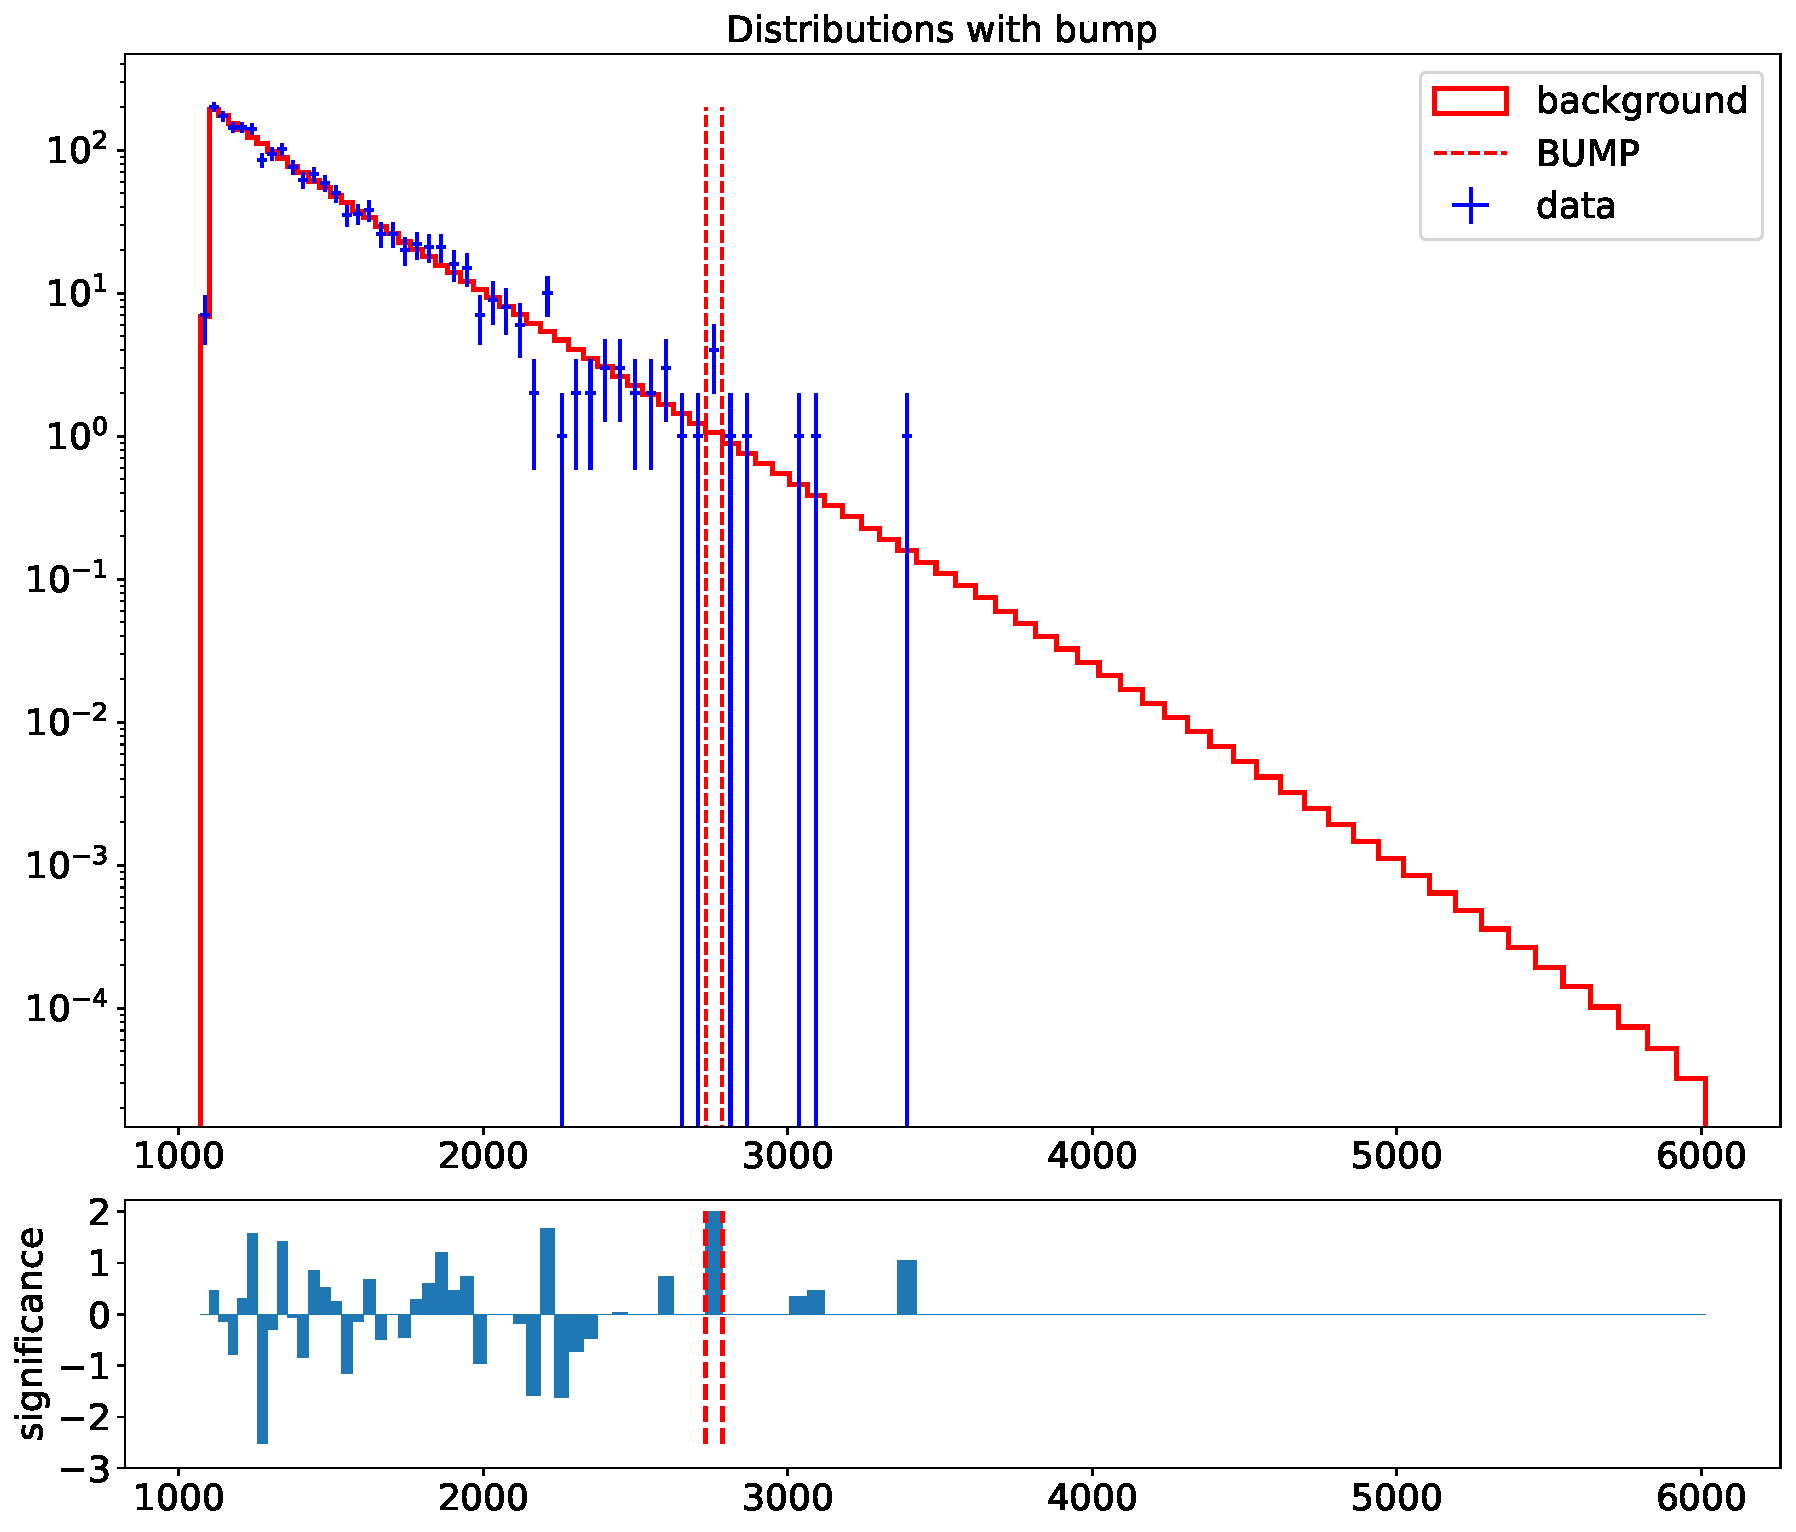
\includegraphics[width=\linewidth]{5_resonances/results/bkgonly/SRB/dof2__range_1100_6000/fits/BHoutput__dof2__data__SRB__asimov_bump}
        \caption{Most significant bump.}
    \end{subfigure}
    \hfill
    \begin{subfigure}[h]{0.49\linewidth}
        \centering
        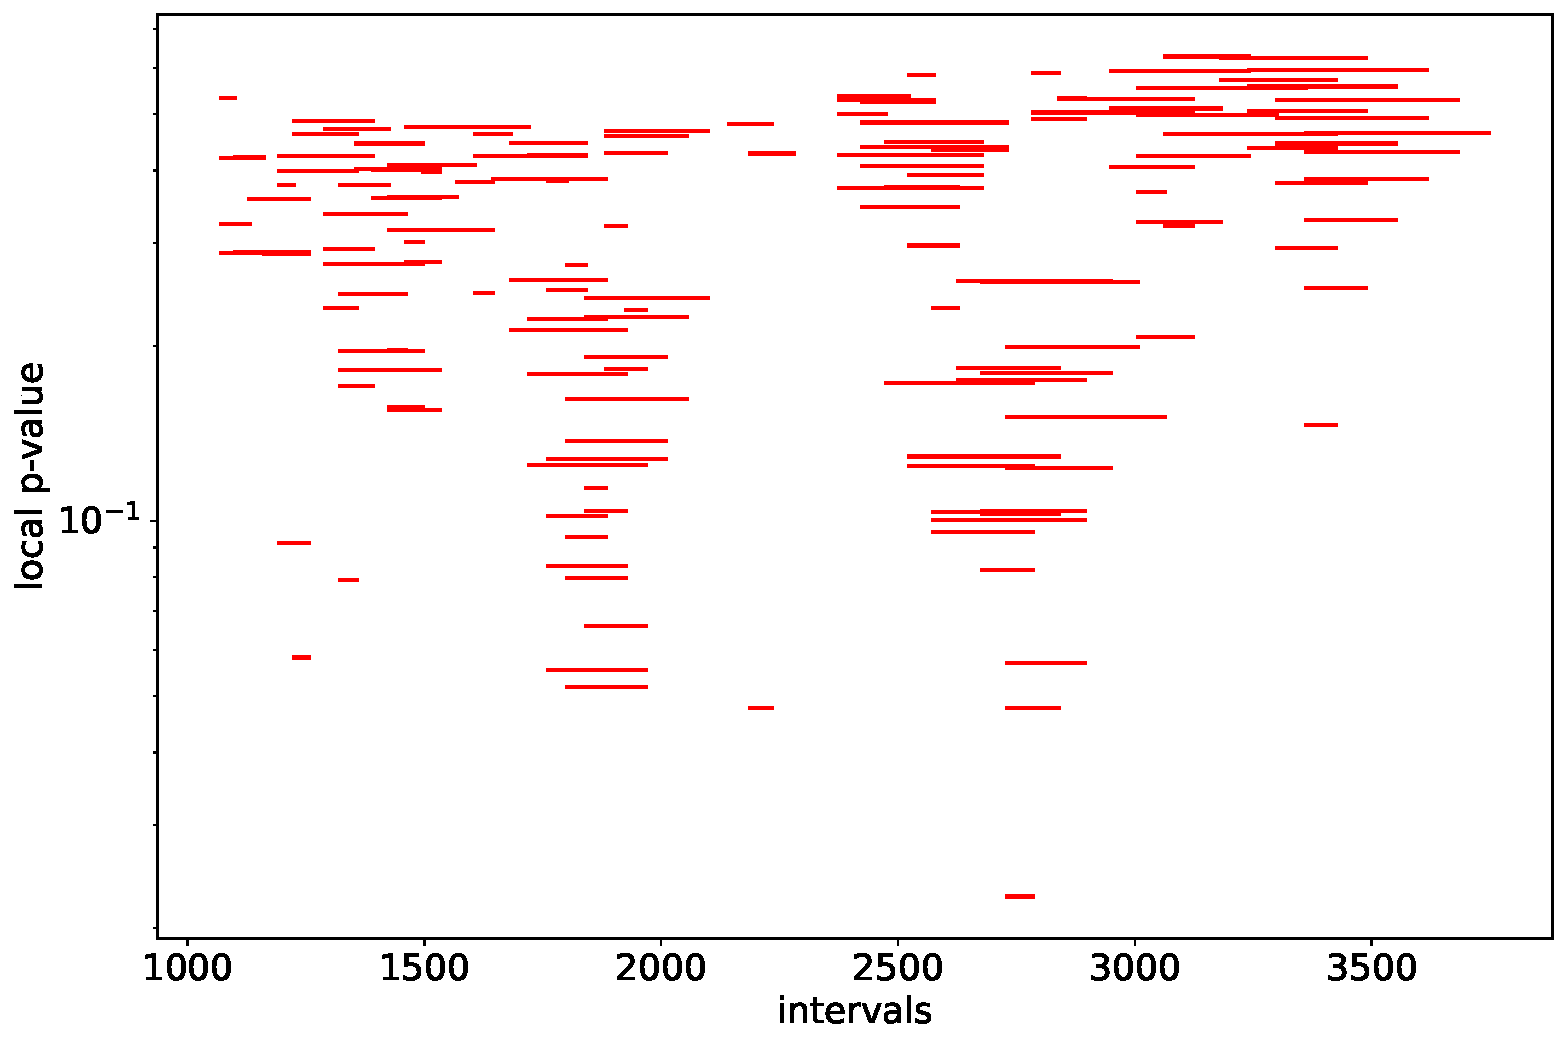
\includegraphics[width=\linewidth]{5_resonances/results/bkgonly/SRB/dof2__range_1100_6000/fits/BHoutput__dof2__data__SRB__asimov_tompgraphy}
        \caption{Tomography scan showing Local \pval.}
    \end{subfigure}
    \caption{Same as \Fig{\ref{fig:results:results:bkgonly:bh:SR}} but in region SRC50, where the resulting global \(p(\text{BH}) = 0.7941\) and significance \(-0.820\).}
    \label{fig:results:results:bkgonly:bh:SRB}
\end{figure}

In all the signal regions, the \bh algorithm manages to find the most significant window in data, but in all cases the significance is either 0 or negative. As discussed in \Sect{\ref{subsec:strategy:stat_treatment:bh}}, a negative significance means the deviation seen in data is less significant than the one observed from pseudo-data.

The fact that the obtained p-values are greater than the thresholds, both when looking in individual windows or in the whole distribution, when comparing the data and \ac{BO} functions, means that an excellent modeling of the background is achieved. Only small differences are seen in the residues of the fits, due to data downwards fluctuations in high-mass regions.
%%%%%%%%%%%%%%%%%%%%%%%%%%%%%%%%%%%%%%%%%%%%%%%%%%%%%%%%%%%%%%%%%%%%%%%%%%%%%%%%%%%%%%%%%%%%%%%%%%%%
%%%%%%%%%%%%%%%%%%%%%%%%%%%%%%%%%%%%%%%%%%%%%%%%%%%%%%%%%%%%%%%%%%%%%%%%%%%%%%%%%%%%%%%%%%%%%%%%%%%%
%%%%%%%%%%%%%%%%%%%%%%%%%%%%%%%%%%%%%%%%%%%%%%%%%%%%%%%%%%%%%%%%%%%%%%%%%%%%%%%%%%%%%%%%%%%%%%%%%%%%



%%%%%%%%%%%%%%%%%%%%%%%%%%%%%%%%%%%%%%%%%%%%%%%%%%%%%%%%%%%%%%%%%%%%%%%%%%%%%%%%%%%%%%%%%%%%%%%%%%%%
%%%%%%%%%%%%%%%%%%%%%%%%%%%%%%%%%%%%%%%%%%%%%%%%%%%%%%%%%%%%%%%%%%%%%%%%%%%%%%%%%%%%%%%%%%%%%%%%%%%%
%%%%%%%%%%%%%%%%%%%%%%%%%%%%%%%%%%%%%%%%%%%%%%%%%%%%%%%%%%%%%%%%%%%%%%%%%%%%%%%%%%%%%%%%%%%%%%%%%%%%
\subsection{Signal interpretation}
\label{subsec:results:results:bkgsig}

The results shown above indicate that no significant bump is observed on the data distributions. For this reason, now a signal-dependent interpretation is presented.

\begin{figure}[ht!]
    \centering
    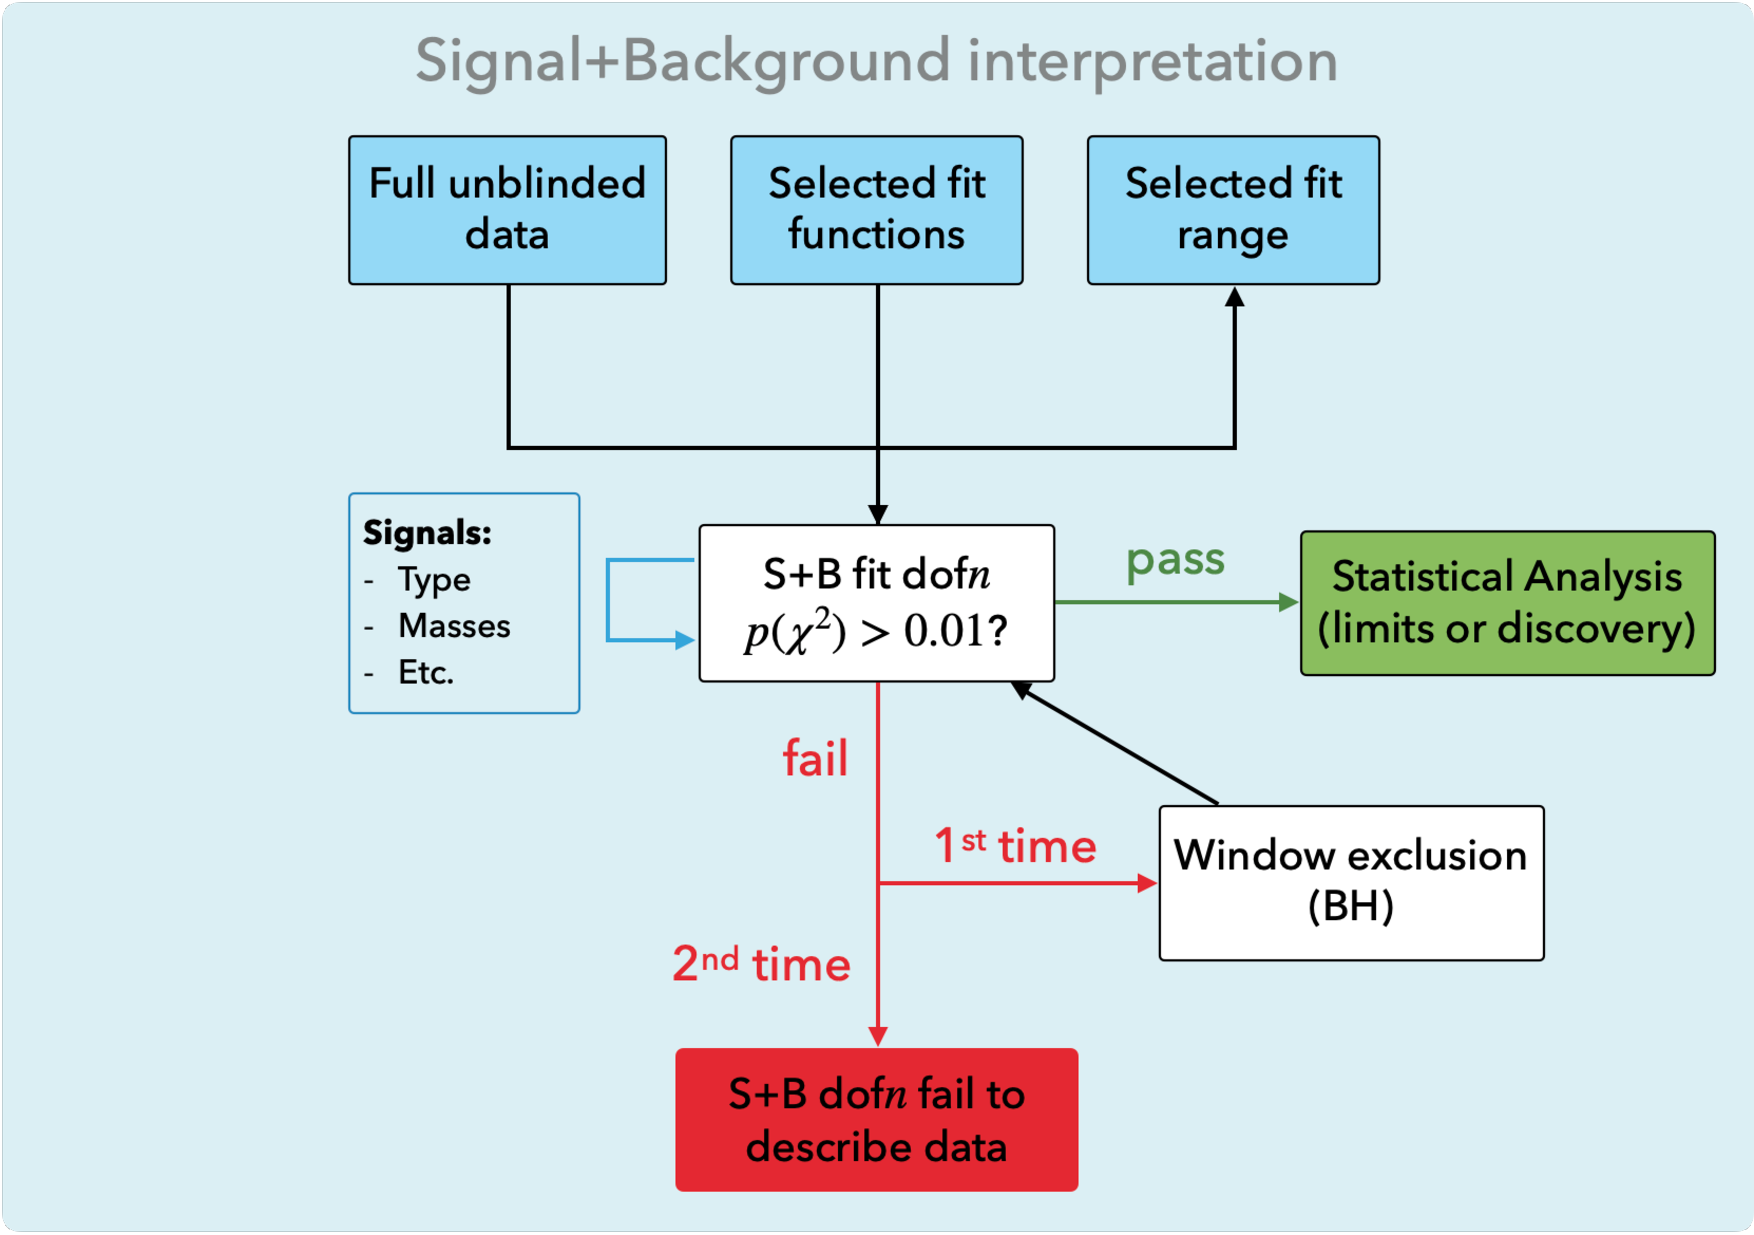
\includegraphics[width=0.7\linewidth]{5_resonances/results/sigbkg/unblind_strategy3_sb}
    \caption{Scheme of the \ac{SB} fit worflow to data.}
    \label{fig:results:results:bkgsig:strat}
\end{figure}

The fitting workflow follows a similar pattern as the one used for the \ac{BO} interpretation (schematised in \Fig{\ref{fig:results:results:bkgsig:strat}}), but is repeated for each one of the considered signal models: \acfp{EQ}, \acfp{QBH}, and generic Gaussians.
First, a \ac{SB} fit is performed on the chosen signal region, followed by a \chisq-test. If the \pval of it passes the threshold of 0.01, a good fit across the entire spectrum is provided and the limit-setting procedure is started. If the threshold is not passed, a local effect other than the signal hypothesis might be the reason. In that case a window exclusion using \bh is applied as described above and the \chisq-test repeated. This path is necessary in order to be able to set limits across the entire \myj range even if a single localized effect would prevent good fits for all other signal hypothesis at different masses. If in this second test \(p(\chisq)\) exceeds the threshold of 0.01, the statistical analysis is continued like in the other path, just with a window masked. If the threshold is not exceeded, the \ac{SB} fit fails to describe the data and no interpretation can be presented.

The goal is to establish limits on the theory's parameters, that is, determine the maximal amount of potential signal for which the \ac{SB} hypothesis \(H_1\) still provides a good description of the data in comparison with the \ac{BO} hypothesis \(H_0\). The limits are computed at \(95\%\) \ac{CL} following the procedure described in \Sect{\ref{subsec:strategy:stat_treatment:hypo_test}}. 


\subsubsection{Results}
\label{subsubsec:results:results:bkgsig:results}

In the following paragraphs, a description of the obtained results is provided for each signal model under consideration in the present thesis.




\paragraph{Excited quarks}
\label{paragraph:results:results:bkgsig:results:qstar}

The \ac{EQ} model proposes a scenario where quarks are not fundamental particles, but rather bound states which decay promptly to a photon and a quark of the same flavor. In this sense, for the first time at the \ac{LHC}, limits on the \ac{EQ} models are separated into three different flavors: \qstar, \cstar and \bstar.
Moreover, the coupling of the \ac{EQ} to the \ac{SM} partners, \(f=f'=f_s\), is kept as a free parameter, therefore limits are computed in the coupling-mass plane, leading to two-dimensional limits.

Exclusion limits are set on the signal cross section \(\sigma_s\) instead of the signal strength \(\mu\). A relation between the two can be found in \Eqn{\ref{eq:strategy:stat_treatment:stat_model:mu_si}}. However, for this model, it is possible to report upper limits on the \(\sigma_s \times \text{Br}\), as the other factors entering \Eqn{\ref{eq:strategy:stat_treatment:stat_model:mu_si}} are known for each signal.

\begin{figure}[ht!]
    \centering
    \begin{subfigure}[t]{0.49\linewidth}
        \centering
        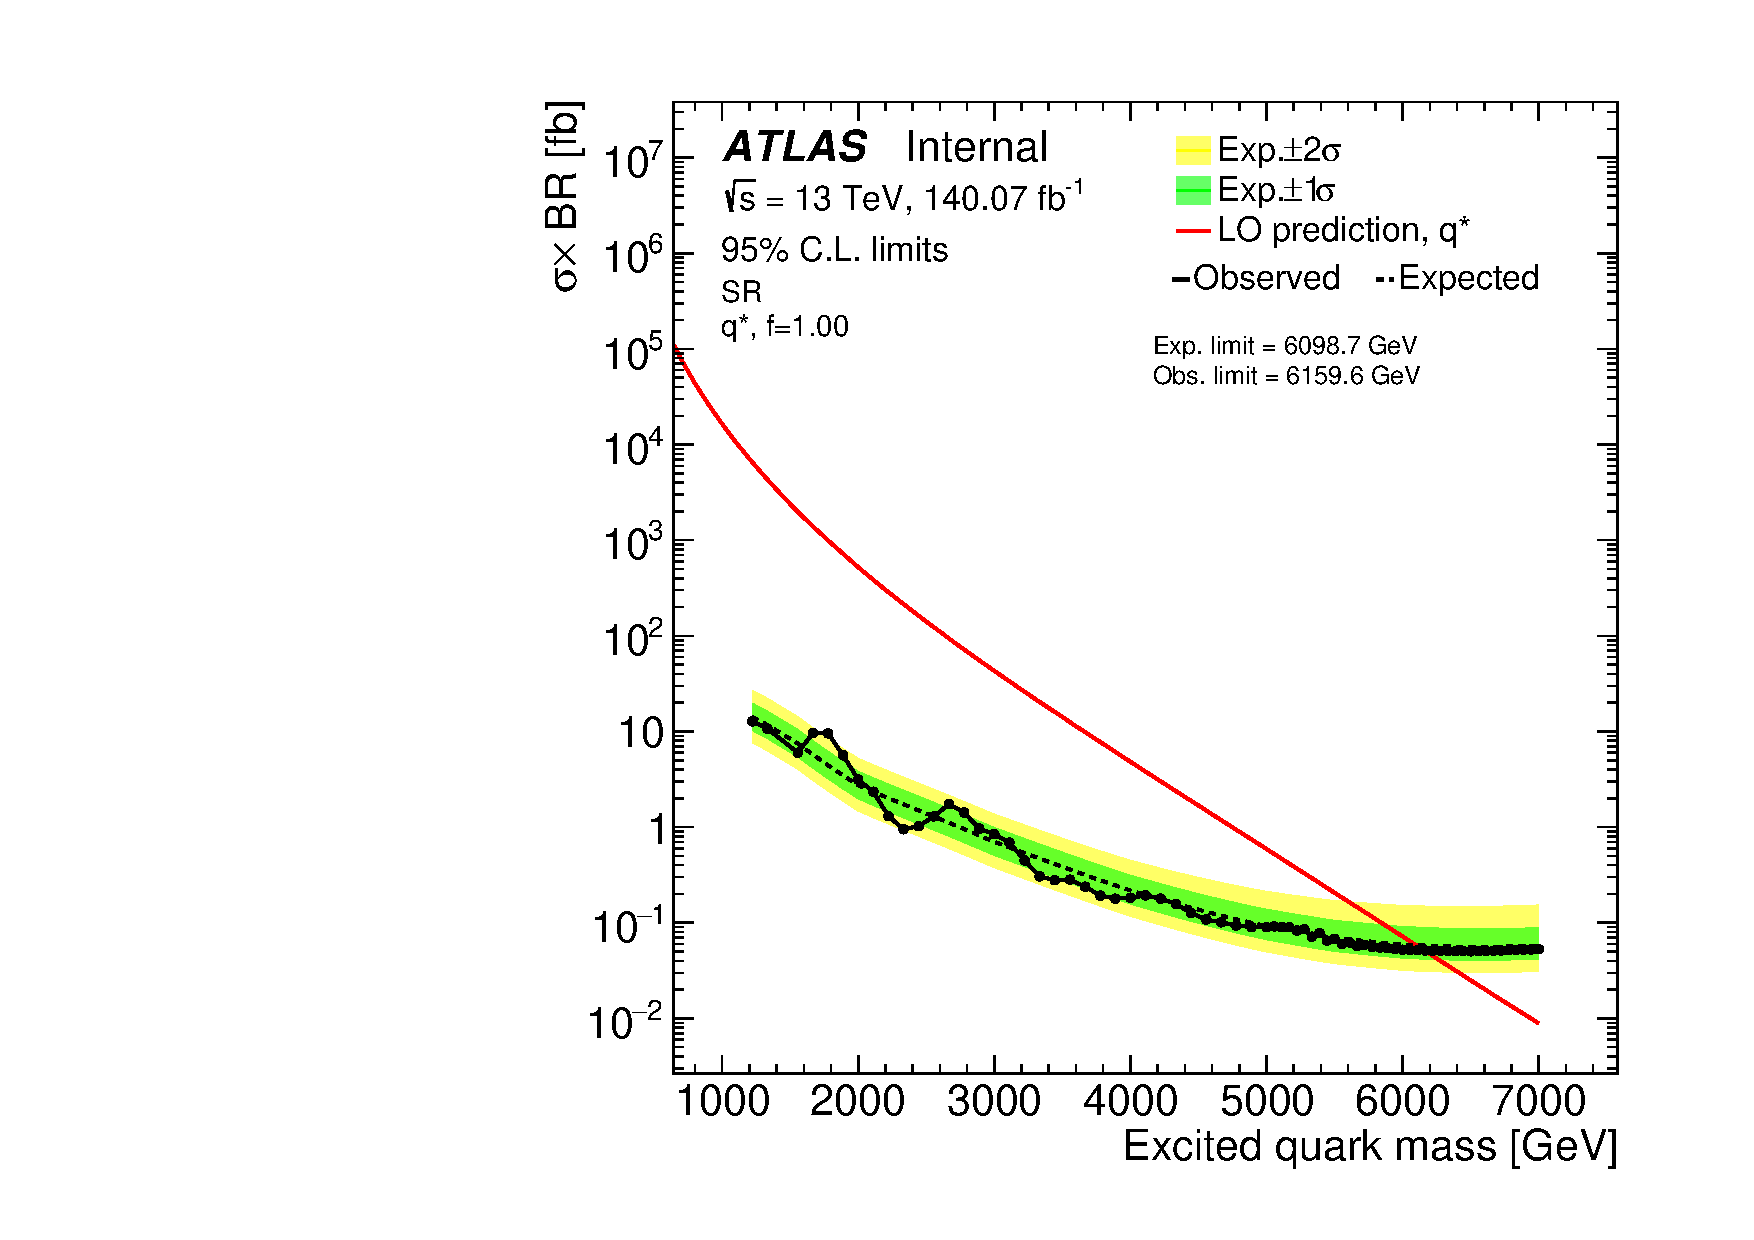
\includegraphics[width=\linewidth]{5_resonances/results/sigbkg/qstar/can__qstar__f1p00__q__SR__qstar__Run2}
        \caption{SR.}
        \label{fig:results:results:bkgsig:results:qstar:limits:SR}
    \end{subfigure}
    \hfill
    \begin{subfigure}[t]{0.49\linewidth}
        \centering
        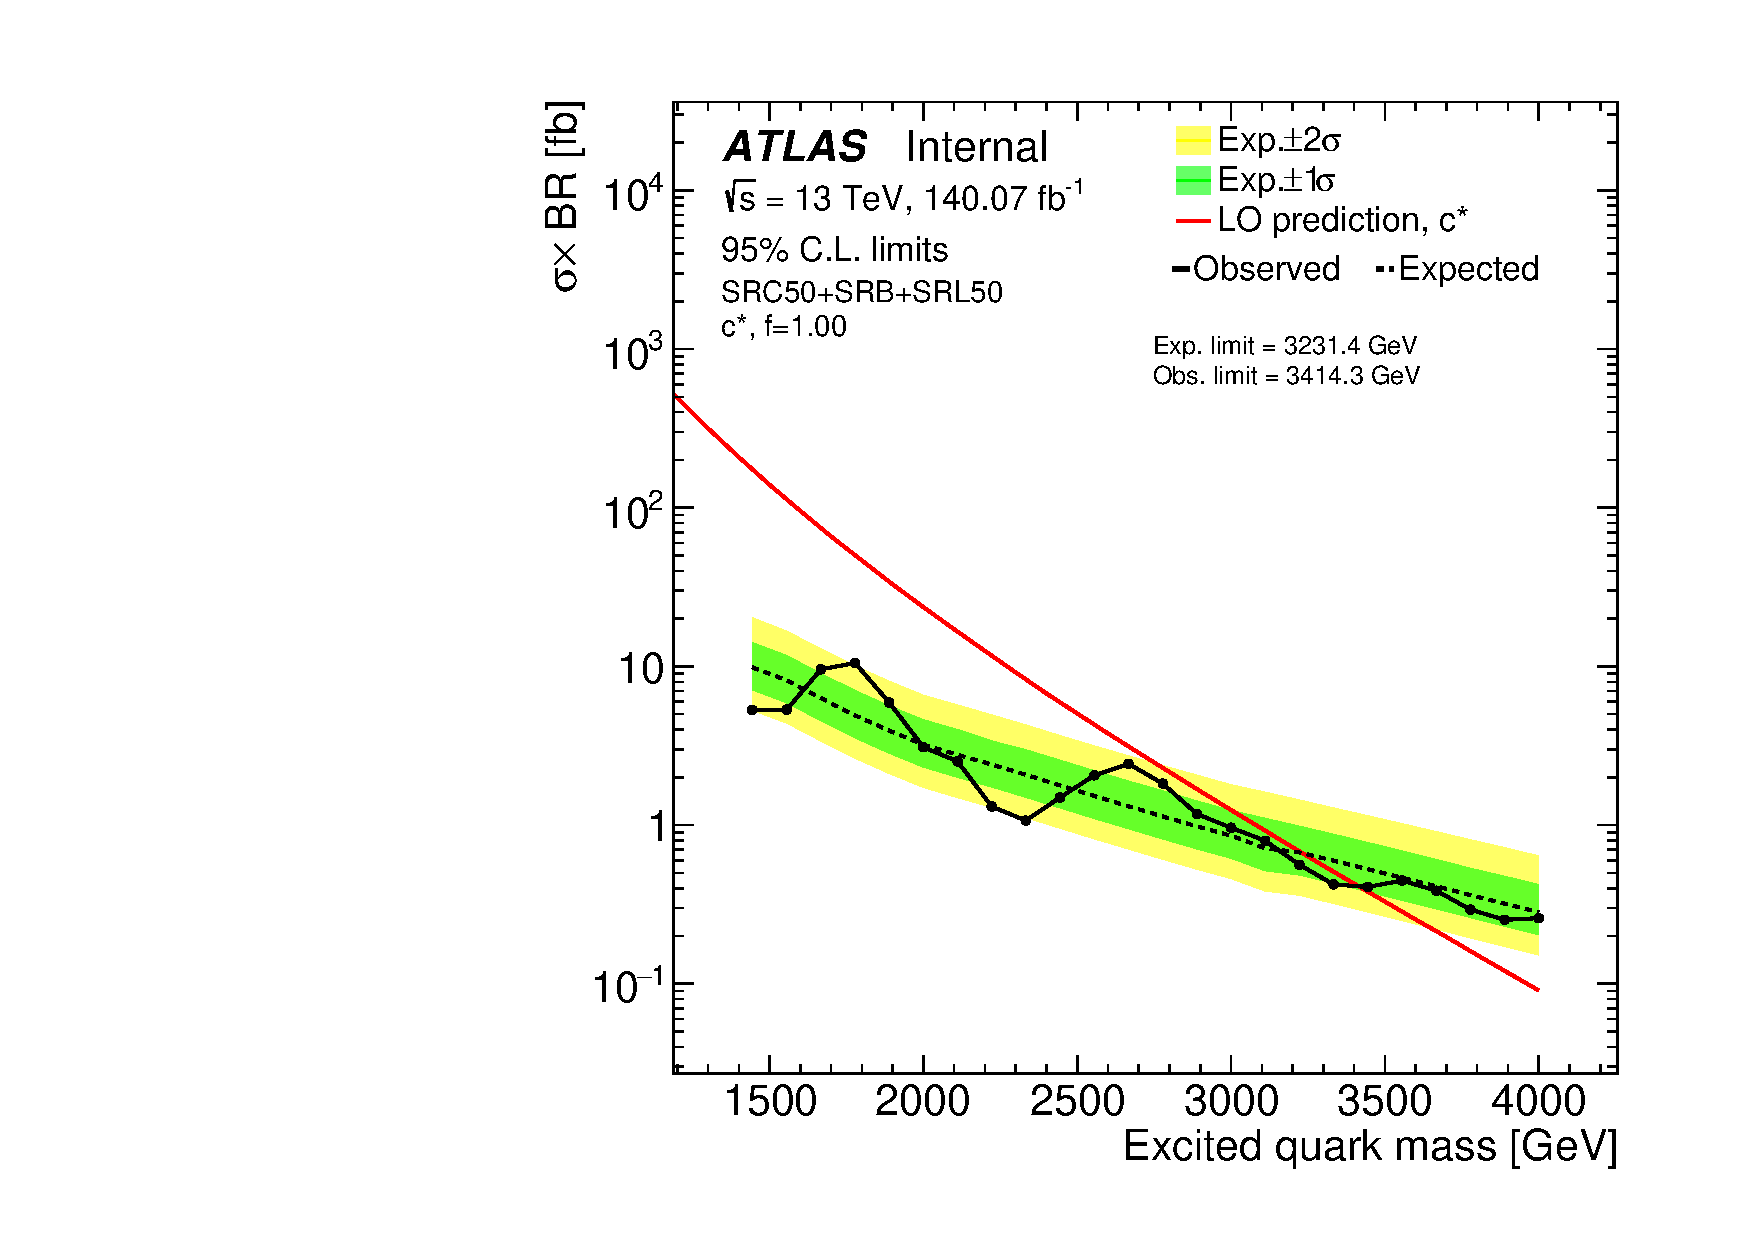
\includegraphics[width=\linewidth]{5_resonances/results/sigbkg/qstar/can__qstar__f1p00__c____qstar__SRC50_SRB_SRL50__Run2}
        \caption{SRC+SRB+SRL.}
        \label{fig:results:results:bkgsig:results:qstar:limits:SRC}
    \end{subfigure}\\
    \begin{subfigure}[t]{0.49\linewidth}
        \centering
        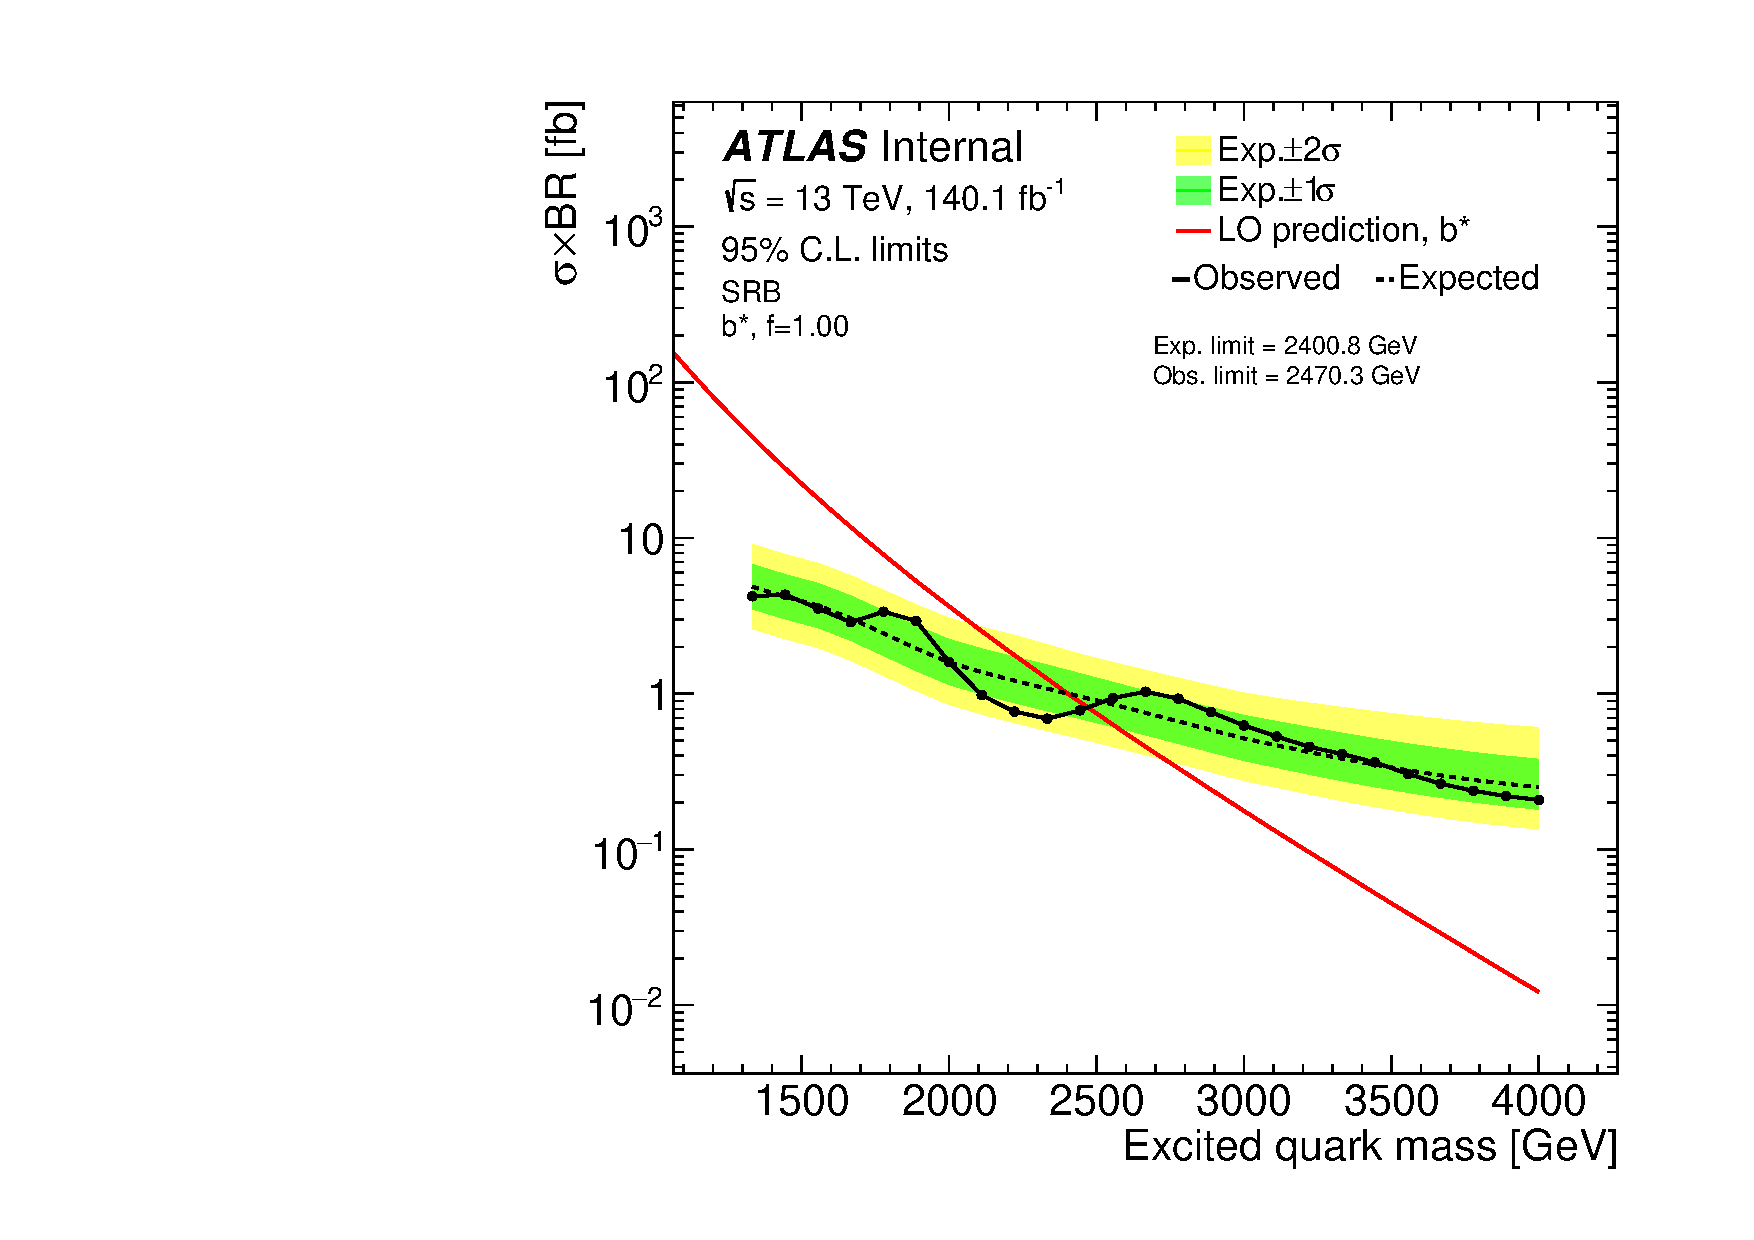
\includegraphics[width=\linewidth]{5_resonances/results/sigbkg/qstar/can__qstar__f1p00__b__SRB__qstar__Run2}
        \caption{SRB.}
        \label{fig:results:results:bkgsig:results:qstar:limits:SRB}
    \end{subfigure}
    \caption{Observed and expected limits on \qstar, \cstar and \bstar signals with coupling \(f=1\), using the full Run-2 dataset. Expected upper limits are shown with the black dashed lines, while the line with marks represent observed limits. Red solid lines indicate the predicted cross section. Marked in the figures, the expected and observed upper limits on the mass are shown.}
    \label{fig:results:results:bkgsig:results:qstar:limits}
\end{figure}

In the case of \qstar signals, the upper limits are obtained in the inclusive region SR, and computed for different coupling values. Results of expected and observed upper limits on \(\sigma_s \times \text{Br}\) are shown in \Fig{\ref{fig:results:results:bkgsig:results:qstar:limits:SR}} for the case of unit coupling. Local observed excesses can be noted at lower masses (\(\sim 1800~\gev\) and \(\sim 2600~\gev\)), but are always within the \(2\sigma\) expected limit uncertainty. These excesses also match exactly the same locations at where the most significant bumps where located by \bh in \Fig{\ref{fig:results:results:bkgonly:bh:SR}}.

For \bstar signals, the specialised SRB region is used. The upper limits are shown in \Fig{\ref{fig:results:results:bkgsig:results:qstar:limits:SRB}}, where again the observed limits behave in the same way as for the SR region: highest deviations away from the expected limits is at masses where the most significant bumps where found using \bh.

Finally, for the first time at the \ac{LHC}, limits on \cstar signals in the \gammajet final state are obtained in this work. The upper limits on \cstar signals are computed in three orthogonal regions simultaneously: SRC, SRB and SRL, and shown for coupling \(f=1\) in \Fig{\ref{fig:results:results:bkgsig:results:qstar:limits:SRC}}. A similar interpretation of the deviations from the expected limits is more difficult in this case, as the simultaneous fit combines the contributions in the three orthogonal regions. However, it is useful to visualise the limits one would get in case of using the \ctagging region SRC alone, compared to the simultaneous limits. This comparison is shown in \Fig{\ref{fig:results:results:bkgsig:results:qstar:limits_SRC_comparison}} where a clear improvement is noted, leading to approximately \(\sim 200~\gev\) increase on the upper limits on the \mc mass.

\begin{figure}[ht!]
    \centering
    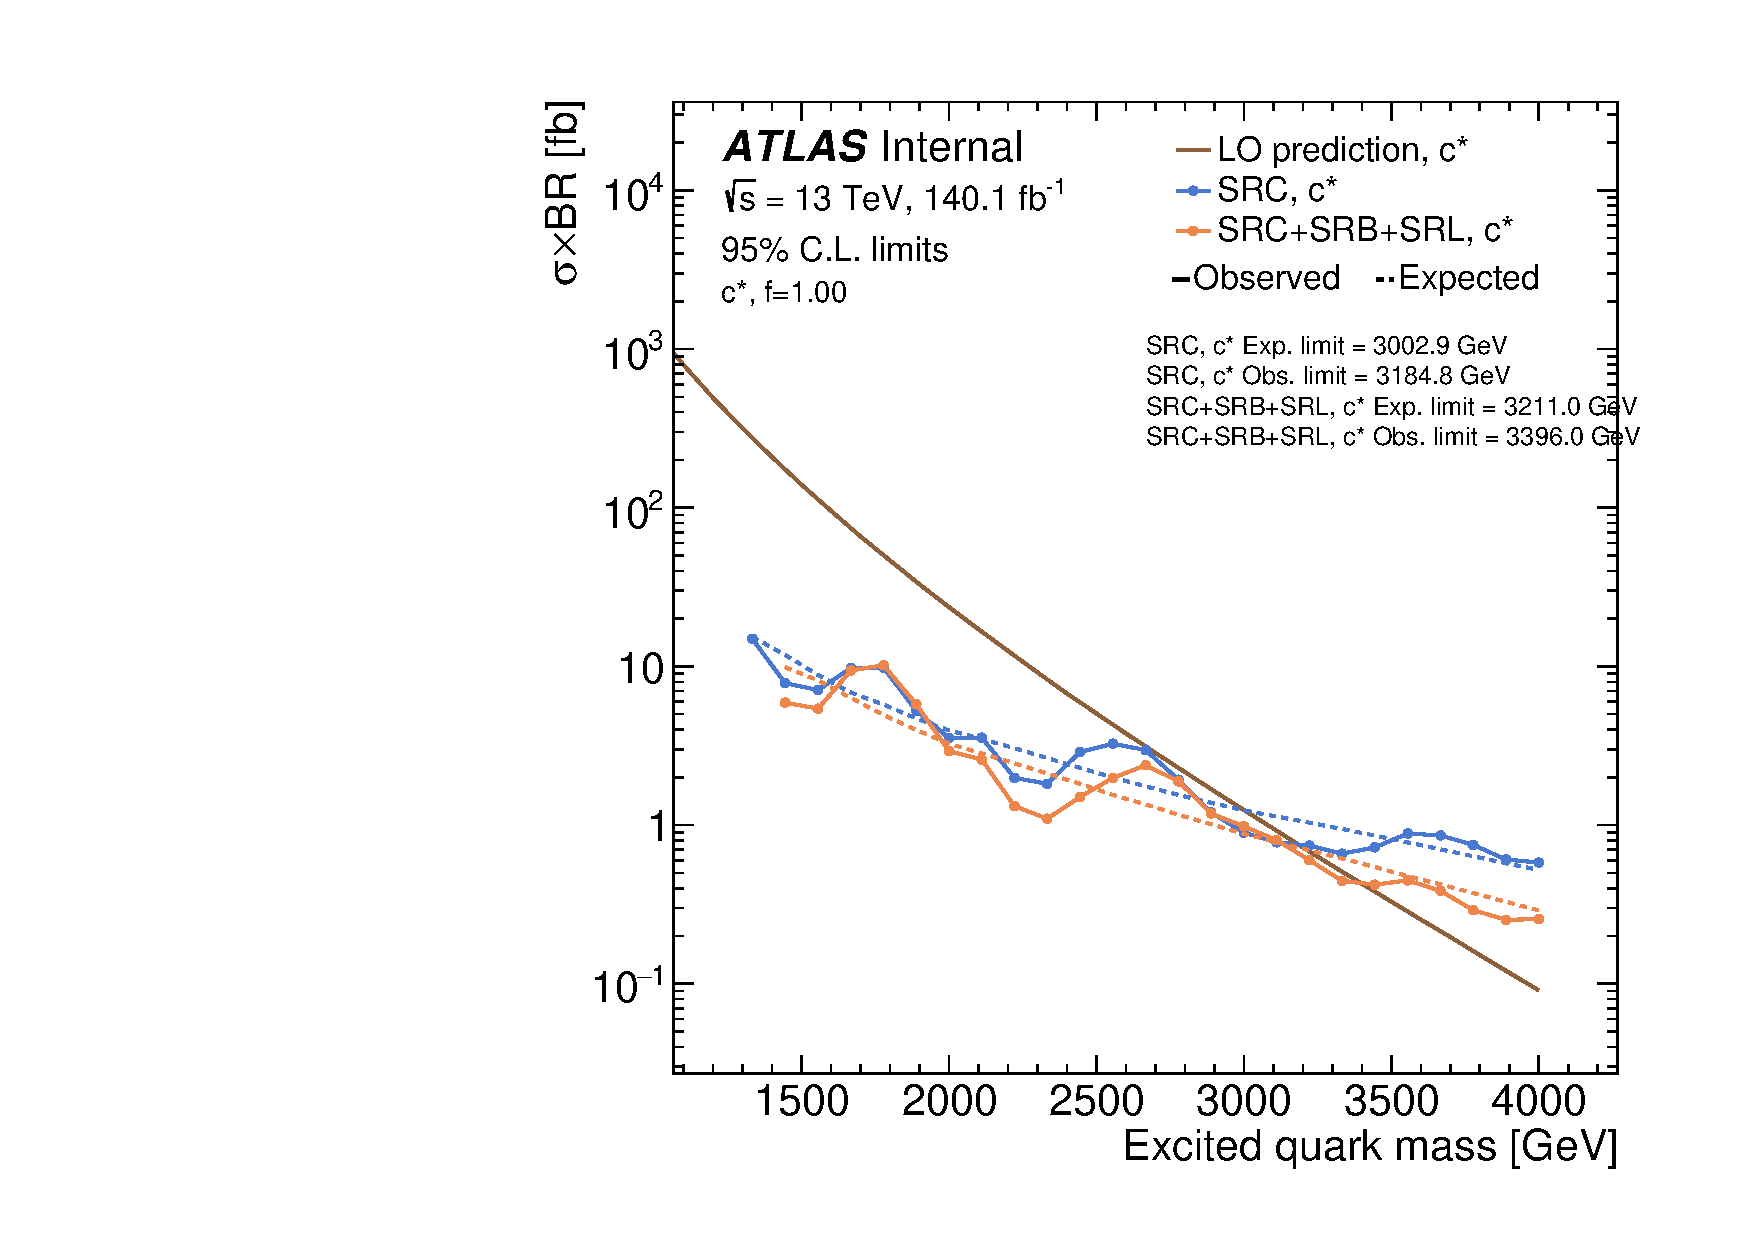
\includegraphics[width=0.49\linewidth]{5_resonances/results/sigbkg/qstar/can__qstar__f1p00__c____qstar__SRC50_SRC50_SRB_SRL50__Run2}
    \caption{Upper limit comparison between the SRC (blue lines) and the SRC+SRB+SRL (orange lines) regions using \cstar signals with coupling \(f=1\). For both regions, the expected and observed upper limit on the \mq mass is displayed in the figure.}
    \label{fig:results:results:bkgsig:results:qstar:limits_SRC_comparison}
\end{figure}

\begin{figure}[ht!]
    \centering
    \begin{subfigure}[t]{0.49\linewidth}
        \centering
        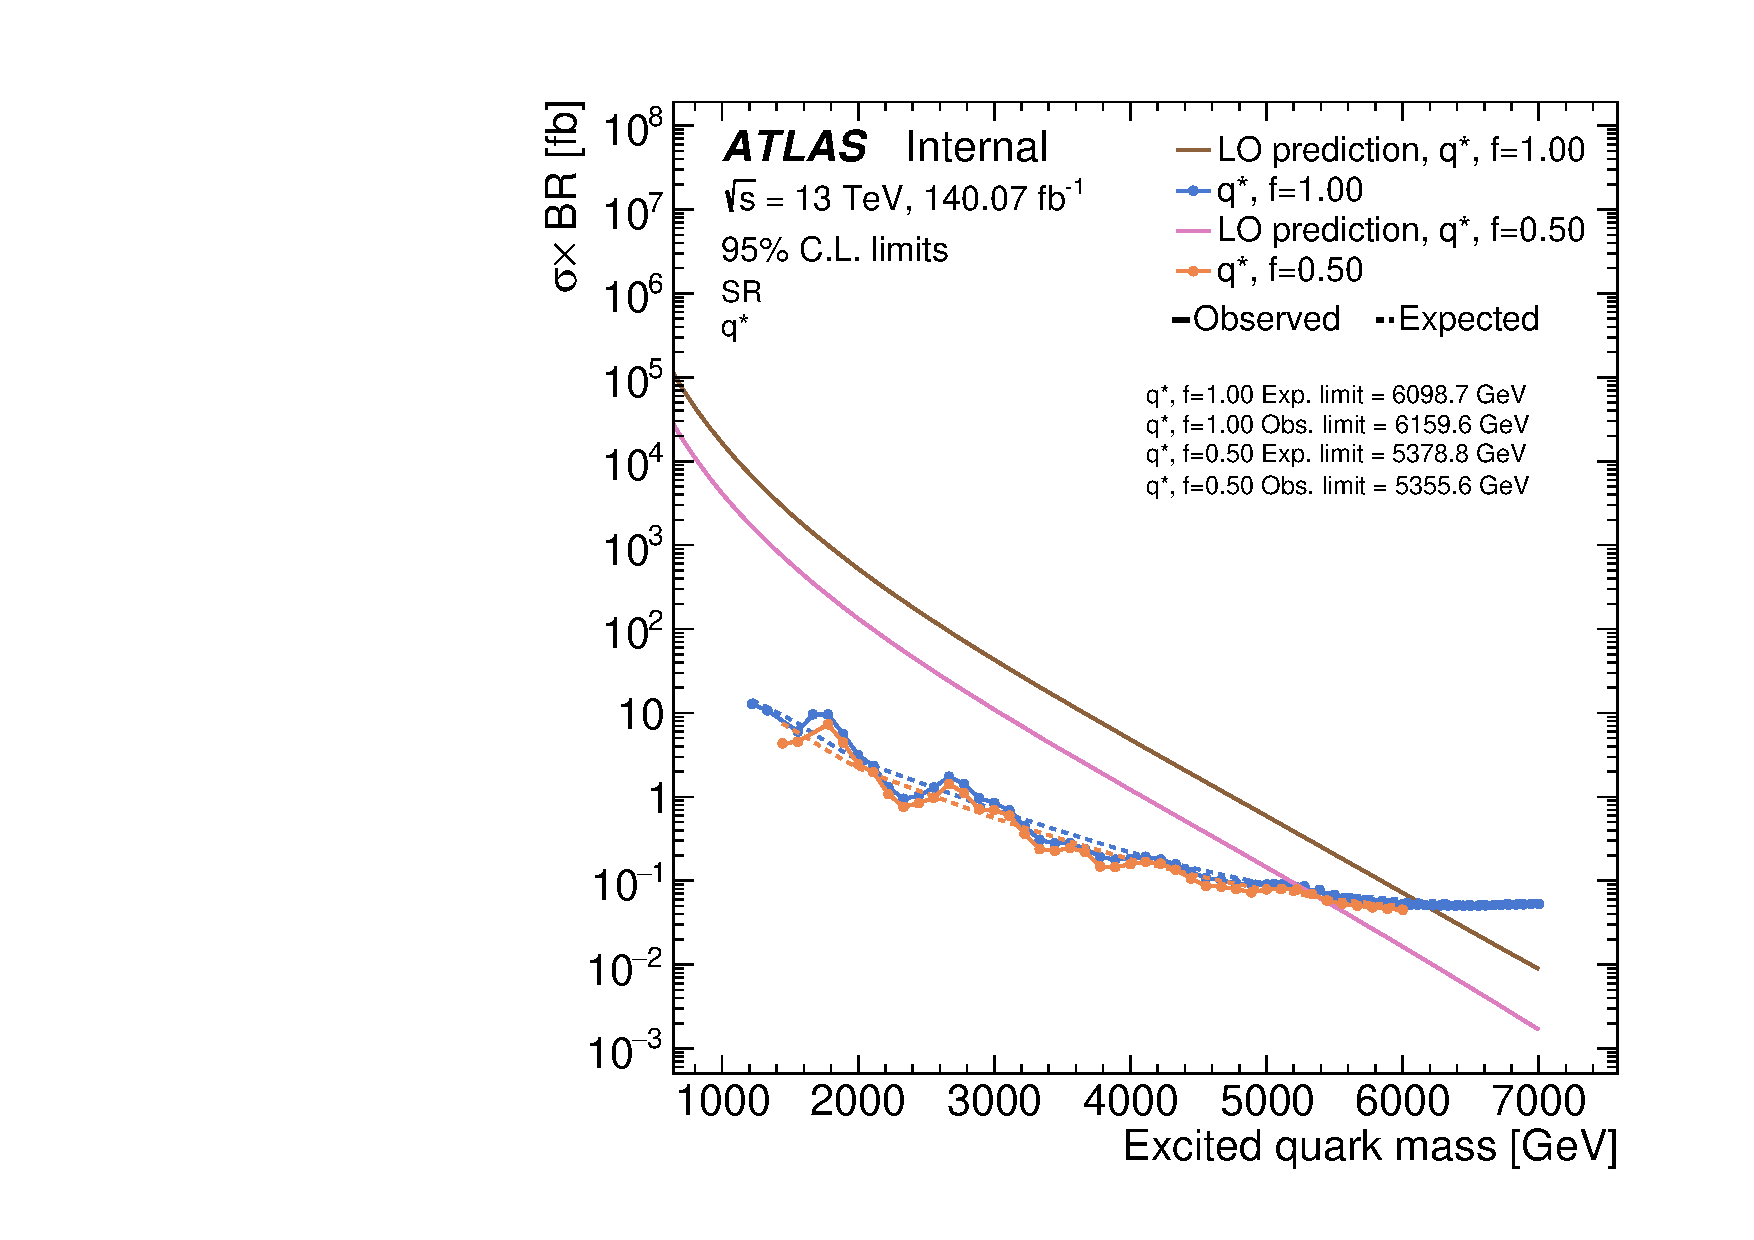
\includegraphics[width=\linewidth]{5_resonances/results/sigbkg/qstar/can__qstar__f1p00__q__SR__qstar__1p0_0p5__Run2}
        \caption{SR.}
        \label{fig:results:results:bkgsig:results:qstar:limits_couplings_comparison:SR}
    \end{subfigure}
    \hfill
    \begin{subfigure}[t]{0.49\linewidth}
        \centering
        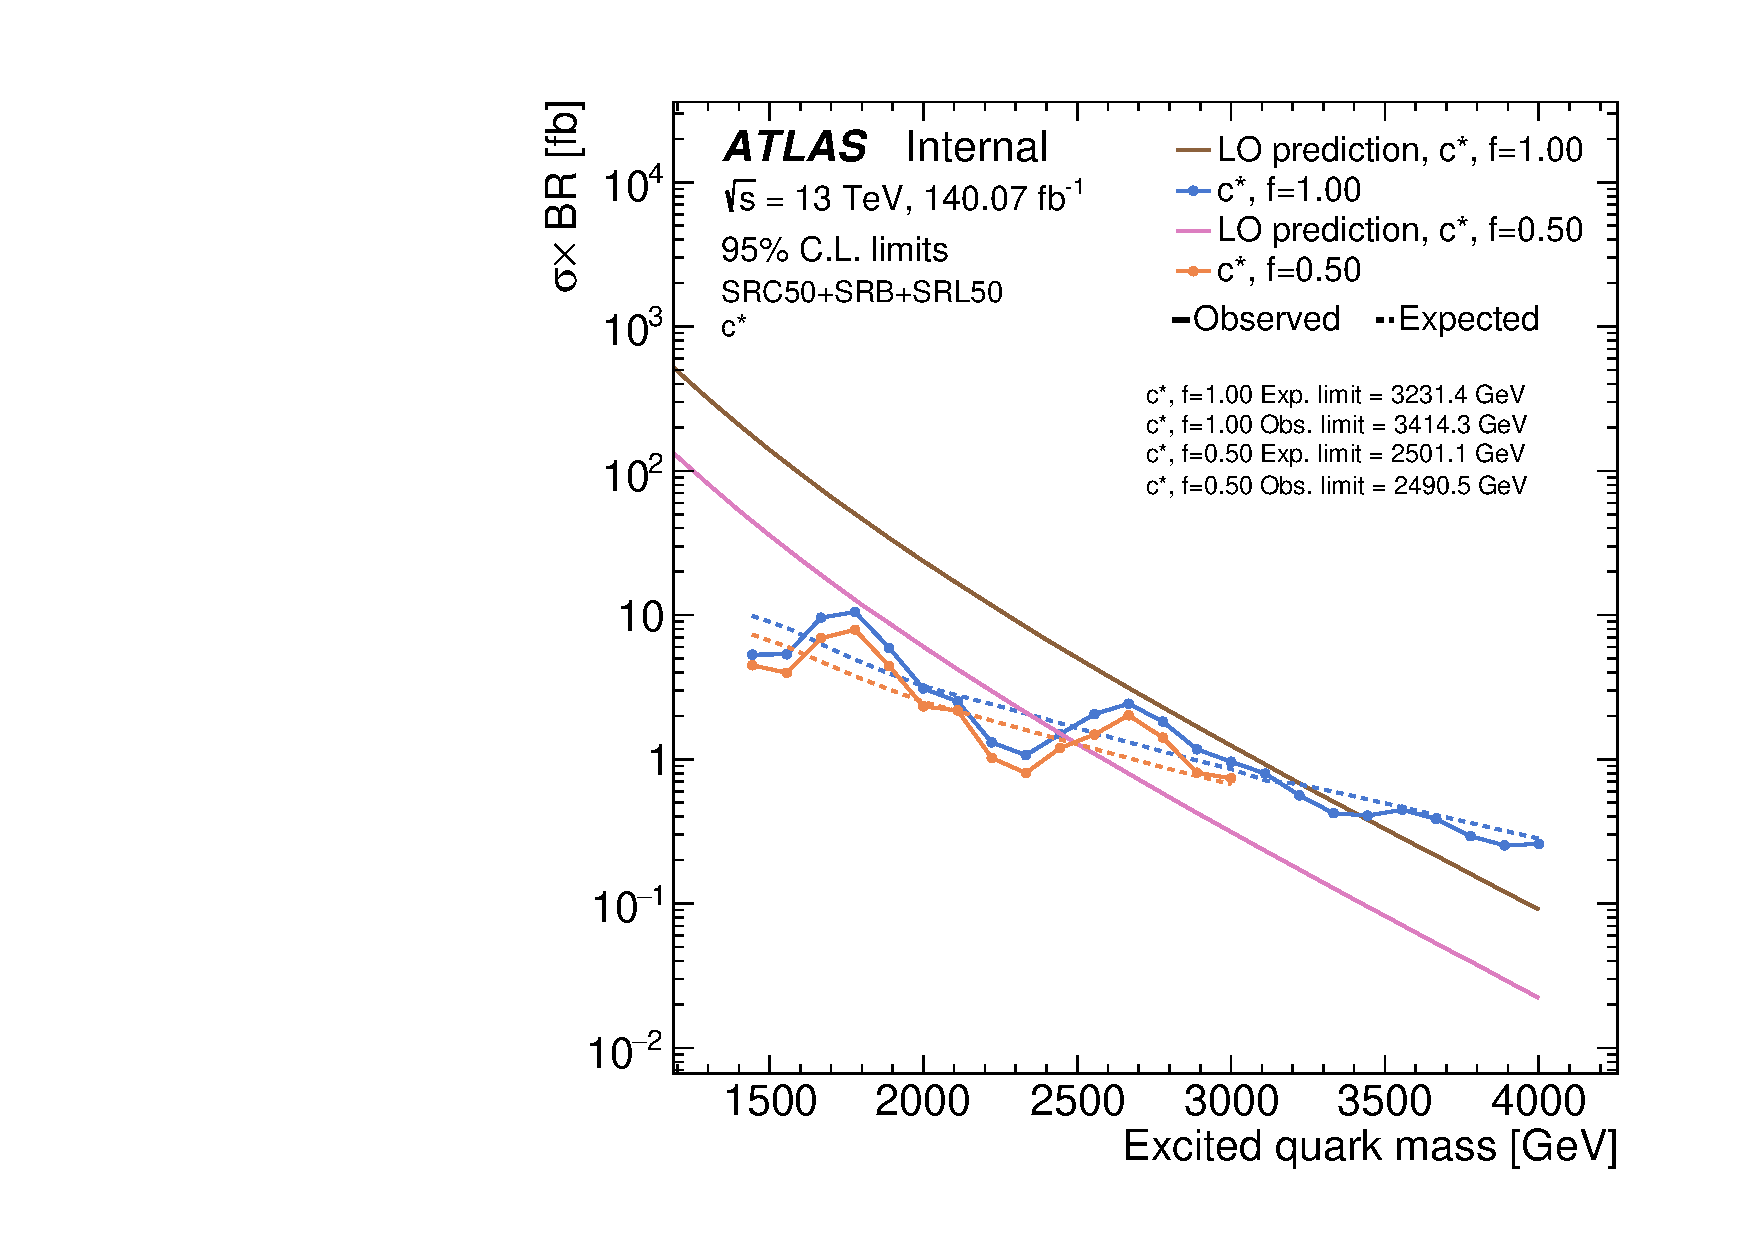
\includegraphics[width=\linewidth]{5_resonances/results/sigbkg/qstar/can__qstar__f1p00__c__SRC50_SRB_SRL50__qstar__1p0_0p5__Run2}
        \caption{SRC50+SRB+SRL50.}
        \label{fig:results:results:bkgsig:results:qstar:limits_couplings_comparison:SRC}
    \end{subfigure}\\
    \begin{subfigure}[t]{0.49\linewidth}
        \centering
        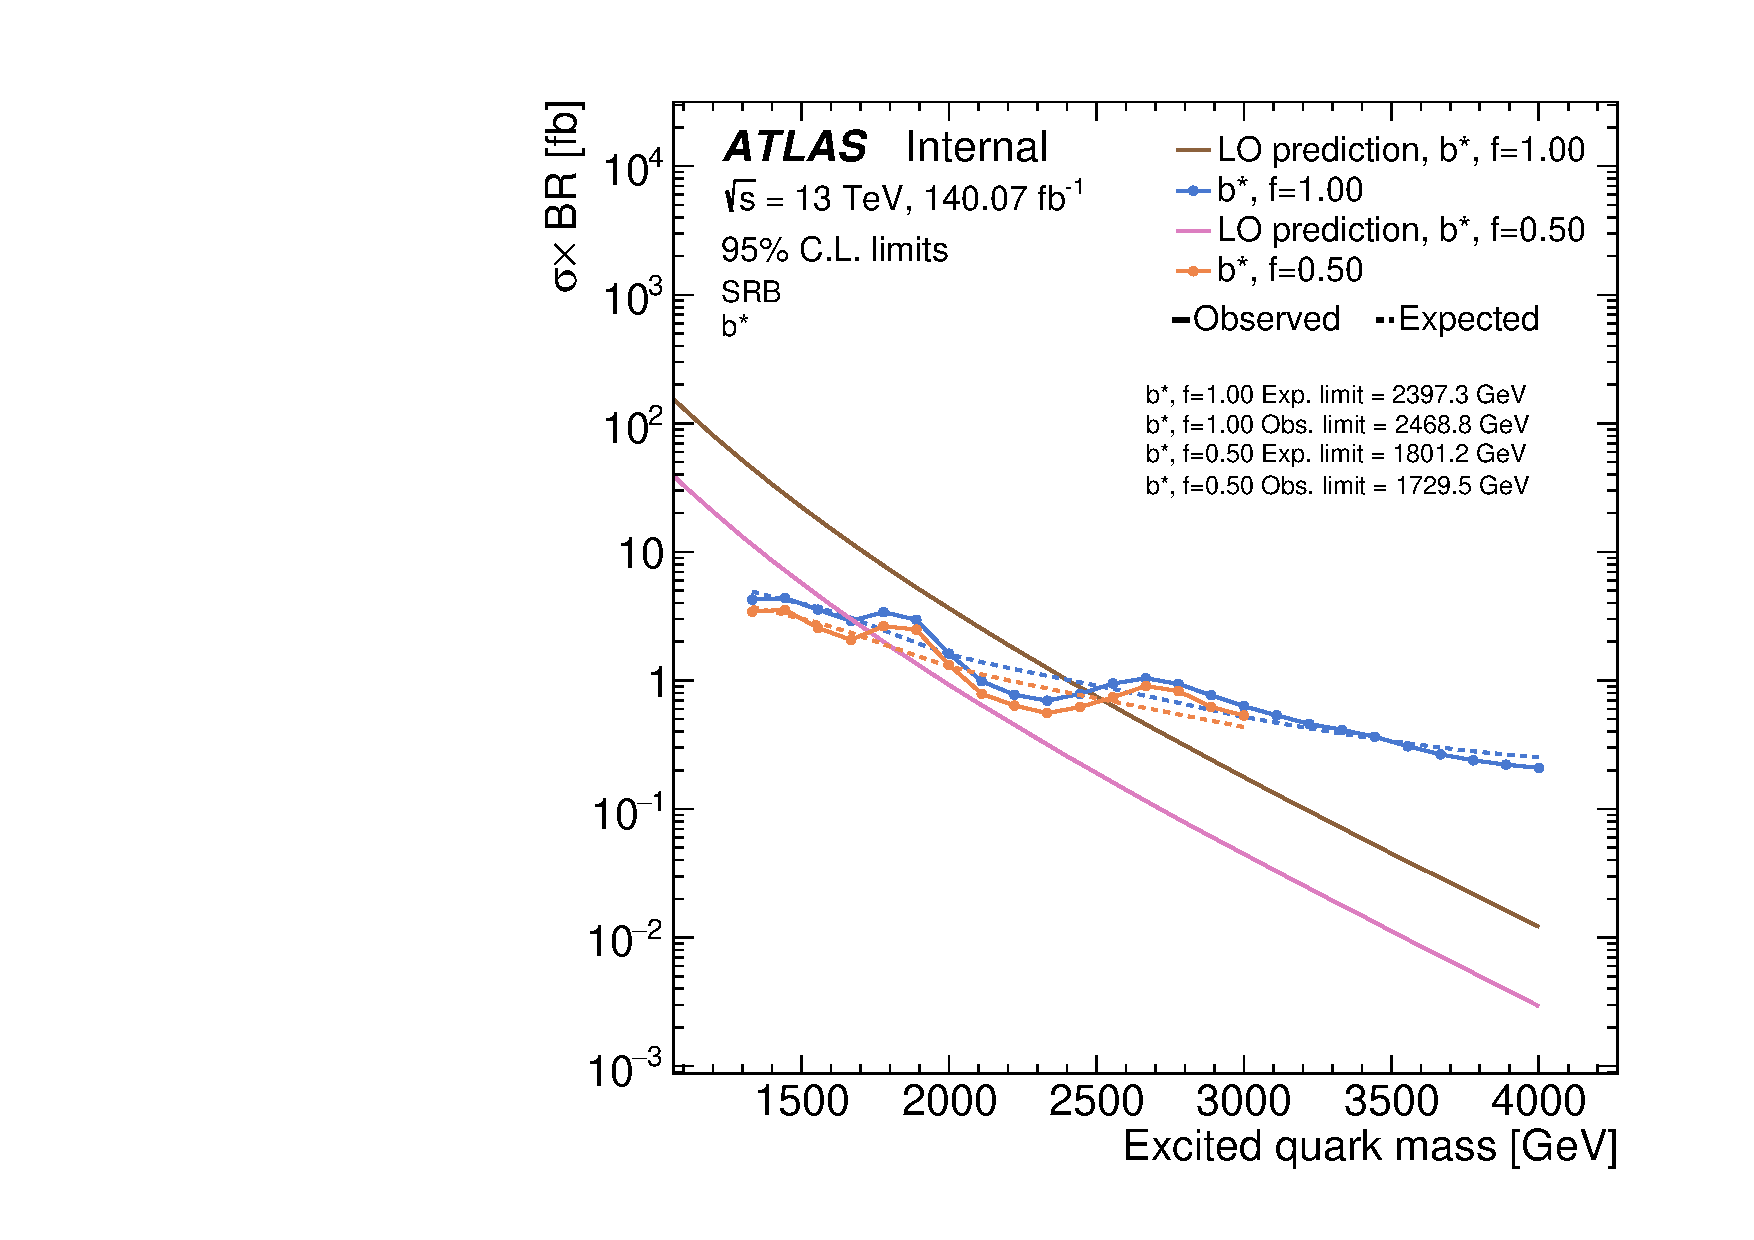
\includegraphics[width=\linewidth]{5_resonances/results/sigbkg/qstar/can__qstar__f1p00__b__SRB__qstar__1p0_0p5__Run2}
        \caption{SRB.}
        \label{fig:results:results:bkgsig:results:qstar:limits_couplings_comparison:SRB}
    \end{subfigure}
    \caption{Observed and expected limits comparison between different couplings for \ac{EQ} signals. Blue (orange) lines represent the limits for coupling \(f=1\) (\(f=0.5\)), and the expected model cross sections are shown with brown (pink) solid lines for \(f=1\) (\(f=0.5\)) signals.}
    \label{fig:results:results:bkgsig:results:qstar:limits_couplings_comparison}
\end{figure}

It is also important to test that the behaviour of the limits for different couplings remains mostly unchanged.
In \Fig{\ref{fig:results:results:bkgsig:results:qstar:limits_couplings_comparison}}, comparisons of the upper limits by using two different coupling values are shown. For all three flavors, the signal with lower coupling always gives the best limits, by a small and (almost) constant factor. This behaviour is in perfect agreement with what is expected given the different acceptances. The \ac{EQ} signals' shapes remain mostly unchanged by varying the coupling, but for \(f\ra 1\), a secondary, off-shell peak appears at lower \myj, leading to slightly lower acceptances.


As previously mentioned, \ac{EQ} upper limits can be represented in the coupling-mass plane, showing the exclusion in these two parameters simultaneously.
In the 2D case, the upper limits on the \(\sigma_s \times \text{Br}\) are represented by a three-dimensional surface, and the upper limits on the parameters are obtained 
In this space, each point representing the expected and observed upper limit is obtained as the intersection of the theory prediction and the calculated upper limit, for a given coupling and mass value. However, the grid granularity is not fine enough to provide a smooth prediction on these values, so a two-dimensional interpolation is necessary. 

However, by virtue of the signal morphing technique presented in \Sect{\ref{sec:signals:modeling}}, it is possible to obtain a much finer 2D-grid from where more accurate limits are computed. After that, a three-dimensional surface is obtained by interpolating the 

In the two-dimensional case, the upper limit on the two parameters is found as the intersection of the theory prediction with the calculated upper limit (\(\sigma_s \times \text{Br}\)).

In spite of that, since the upper limit value is found at the intersection of the theory prediction with the \(\mu\) value, the obtained granularity is not sufficient to obtain a smooth prediction on the upper limits. For this reason, it is necessary to interpolate the upper limits, obtaining a 3D surface, while doing the same for the signal prediction. The intersection of both surfaces will indicate the upper limit value of the theory.



% The upper limit on the mass is computed from the intersection of the theory prediction with the limits on \(\sigma\times \text{Br}\) and are shown in the figures.

The upper limits are also shown in the coupling-mass two-dimensional plane in \Fig{\ref{fig:results:results:bkgsig:results:qstar:limits_2d}}. The figure shows the observed and expected \(95\%\) \ac{CL} upper limits (with the \(\pm 1 \sigma\) uncertainty band) for the three considered flavors, in their respective regions. As expected the limits on the \qstar model are approximately two times more strict than for the \cstar model. In turn, the \cstar upper limits are stricter than for the \bstar signal. This hierarchy on the limits is a consequence primarily on the cross-section of the processes, as lower cross-sections are expected for the heavier resonances. 

\begin{figure}[ht!]
    \centering
    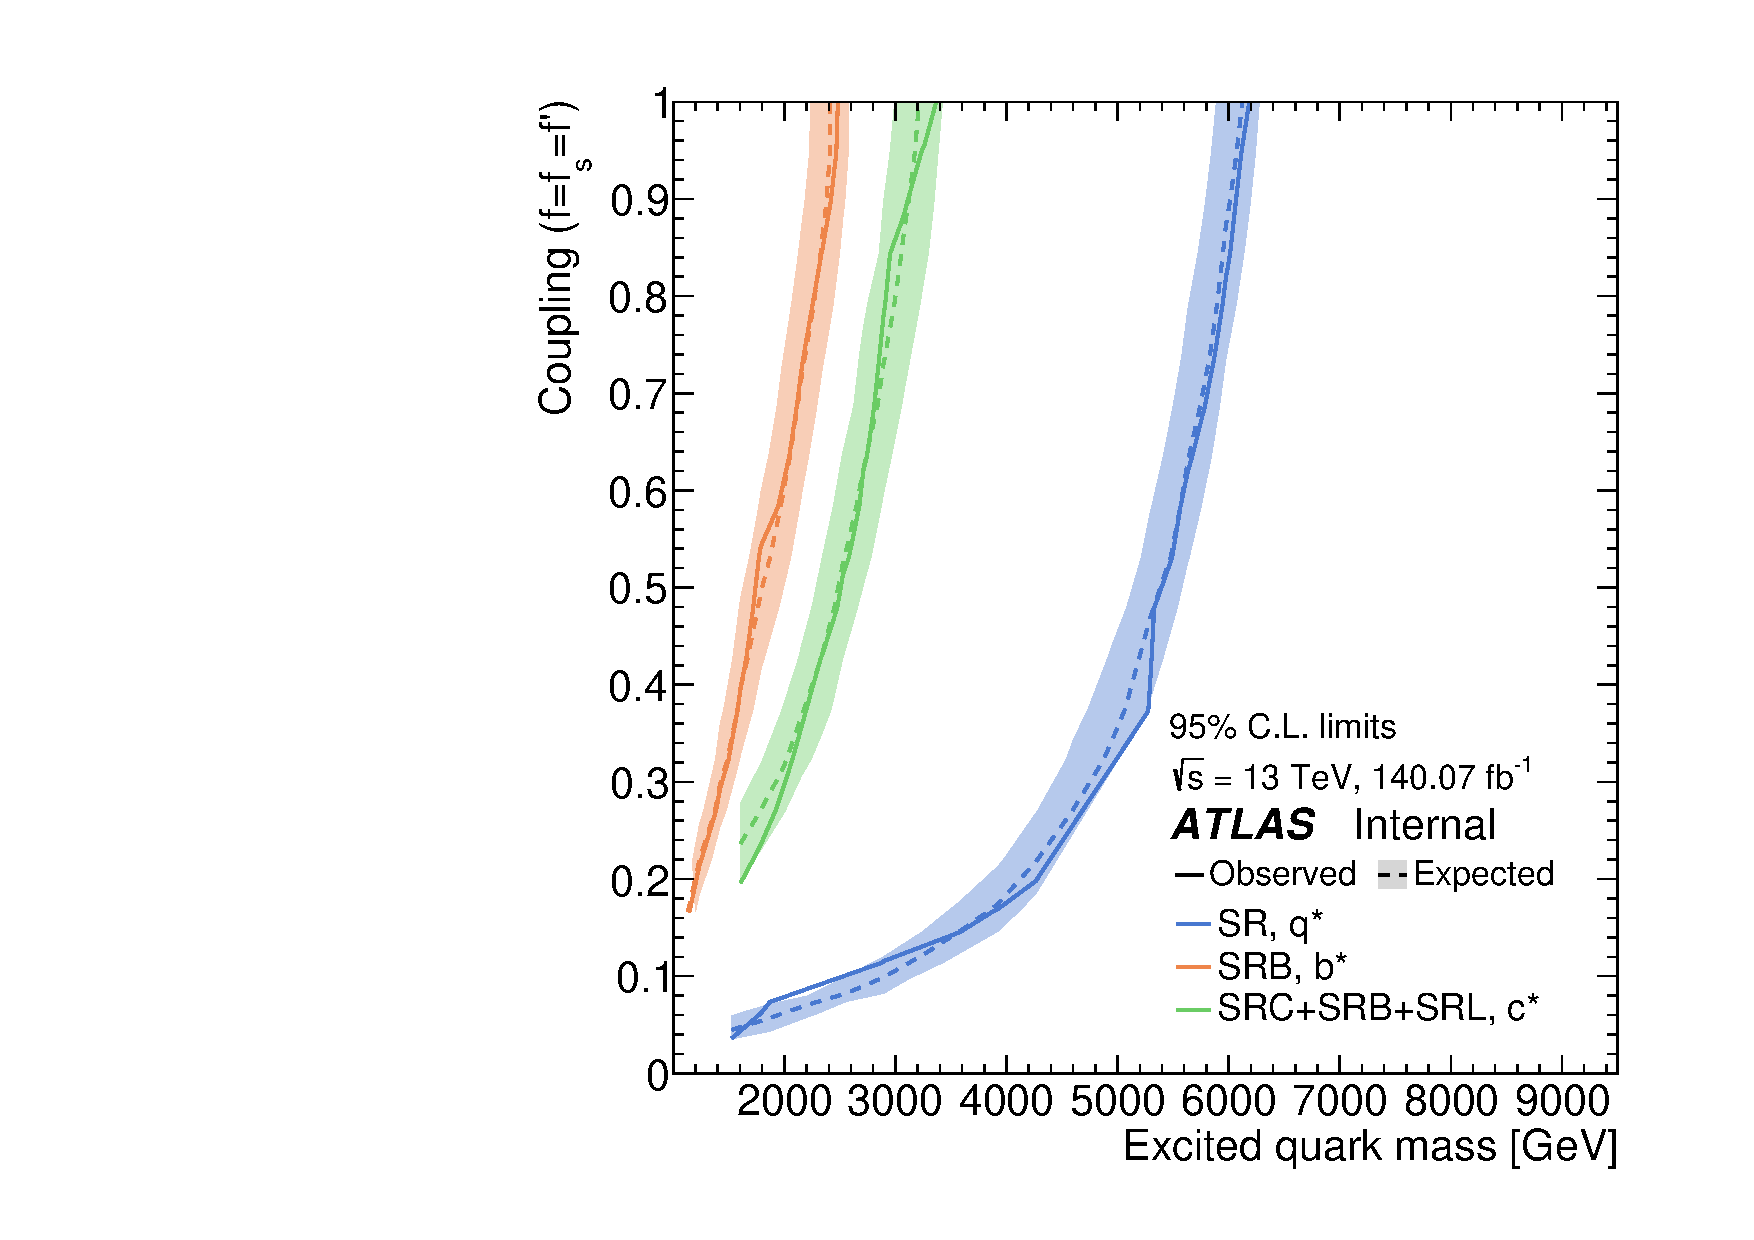
\includegraphics[width=0.7\linewidth]{5_resonances/results/sigbkg/qstar/can__qstar__q_b_c____qstar__SR_SRB_SRC50_SRB_SRL50__Run2}
    \caption{Expected and observed upper limits in the mass-coupling plane for the \qstar (SR), \bstar (SRB) and \cstar (SRC50+SRB+SRL50) signals. The expected (observed) upper limits are displayed with dashed (solid) lines, and the \(1\sigma\) uncertainty band is represented by the colored shaded regions.}
    \label{fig:results:results:bkgsig:results:qstar:limits_2d}
\end{figure}


As of now, these upper limits are the most stringent up to date for the \gammajet final state. At unit coupling, the data exlude \qstar, \cstar and \bstar models with masses up to \(6174.9\), \(3414.3\) and \(2493.7~\gev\), respectively.



\paragraph{Quantum Black Holes}
\label{paragraph:results:results:bkgsig:results:qbh}

Similarly as for \ac{EQ} exclusion limits, for \ac{QBH}, the upper limits are reported on the cross-section times branching ratio \(\sigma_s \times \text{Br}\).
The results on the observed and expected limits for the two \ac{QBH} models (RS1 and ADD) are shown in \Fig{\ref{fig:results:results:bkgsig:results:qbh:limits}}. Following the fitting strategies summary presented in \Tab{\ref{tab:bkg:modeling:strategy_modeling:summary}}, \ac{QBH} signals are only searched for in the inclusive SR. Similarly to what was seen in the case of \ac{EQ} signals, observed limits at \(\sim 1800~\gev\) and \(\sim 2600~\gev\) present deviations up to \(2\sigma\), due to the local, but not significant, excesses found on data with \bh.

\begin{figure}[ht!]
    \centering
    \begin{subfigure}[h]{0.49\linewidth}
        \centering
        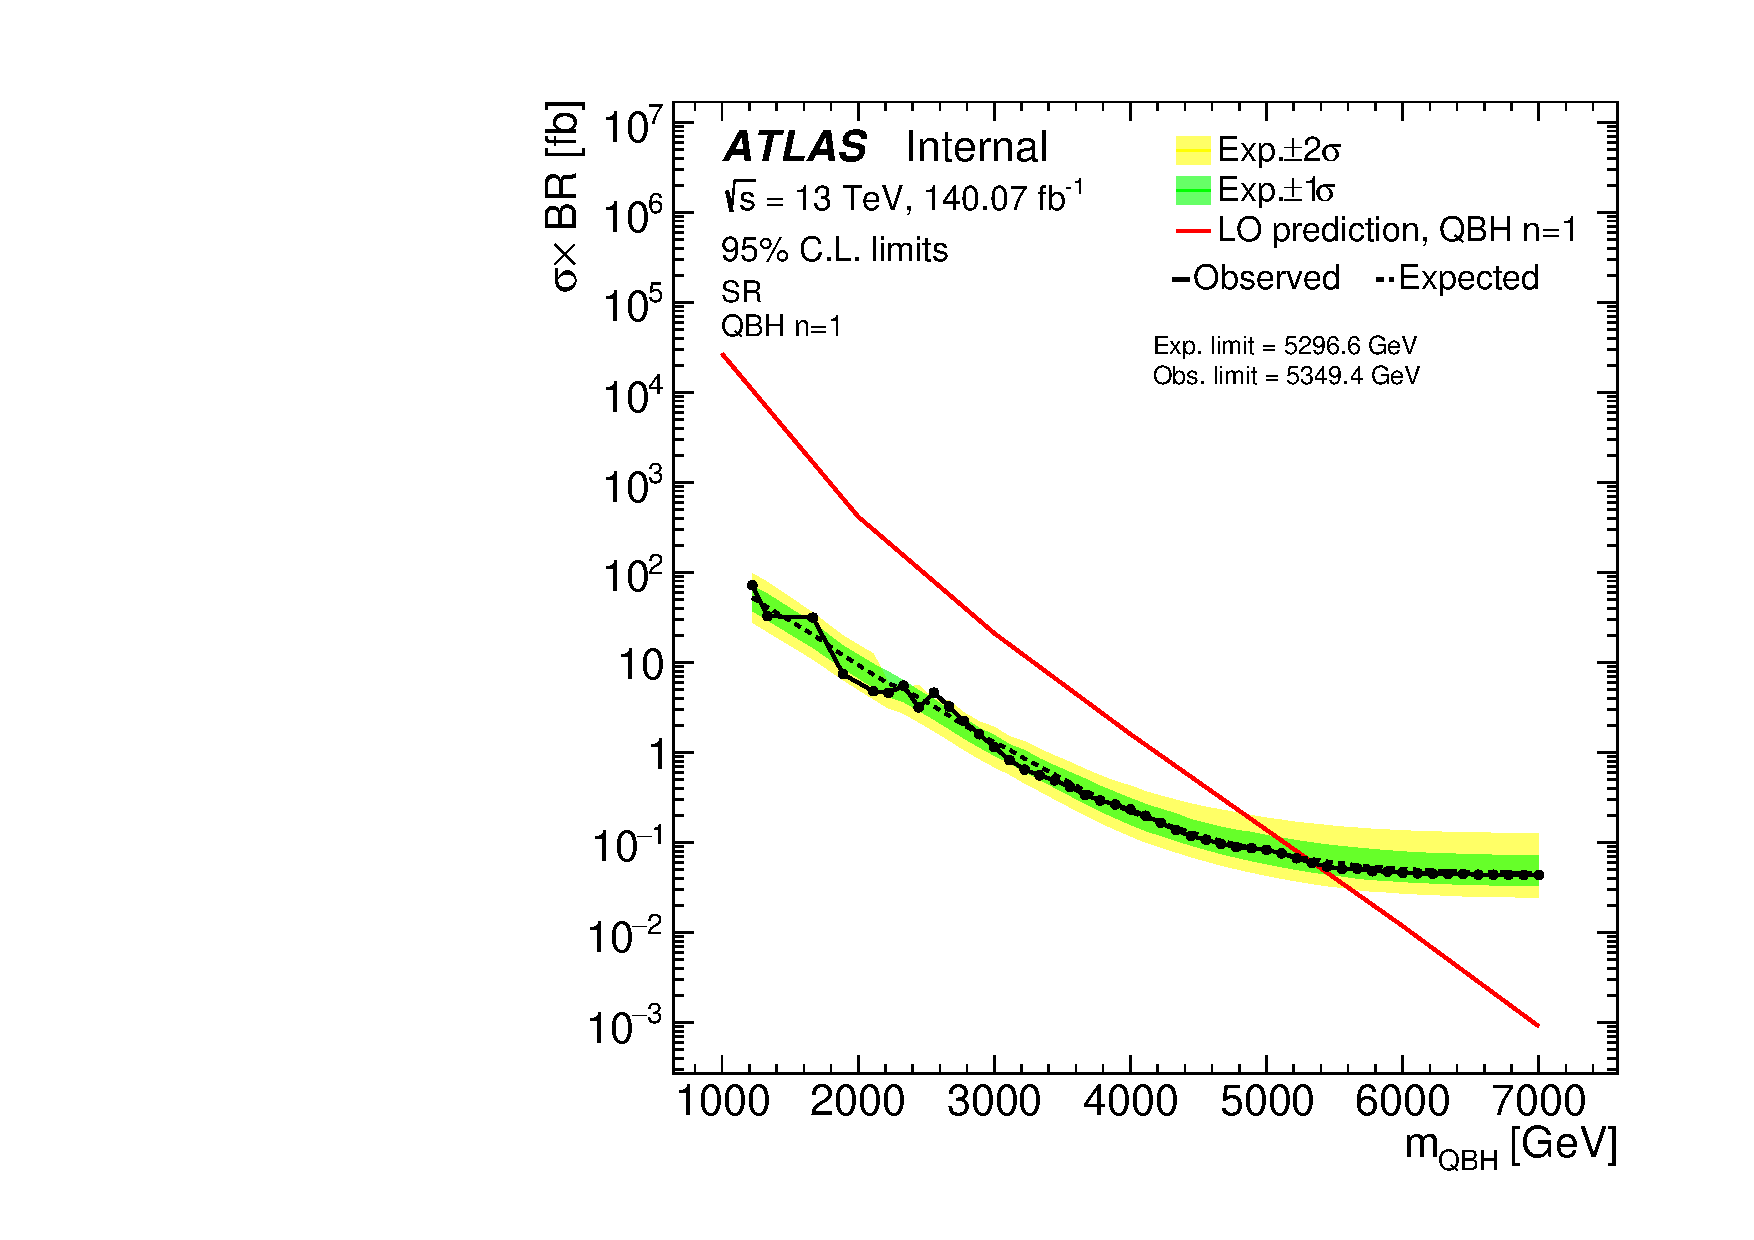
\includegraphics[width=\linewidth]{5_resonances/results/sigbkg/QBH/n1/can__QBH__n1__n1____QBH__SR__Run2}
        \caption{RS1 (\(n=1\)) \ac{QBH} model.}
    \end{subfigure}
    \hfill
    \begin{subfigure}[h]{0.49\linewidth}
        \centering
        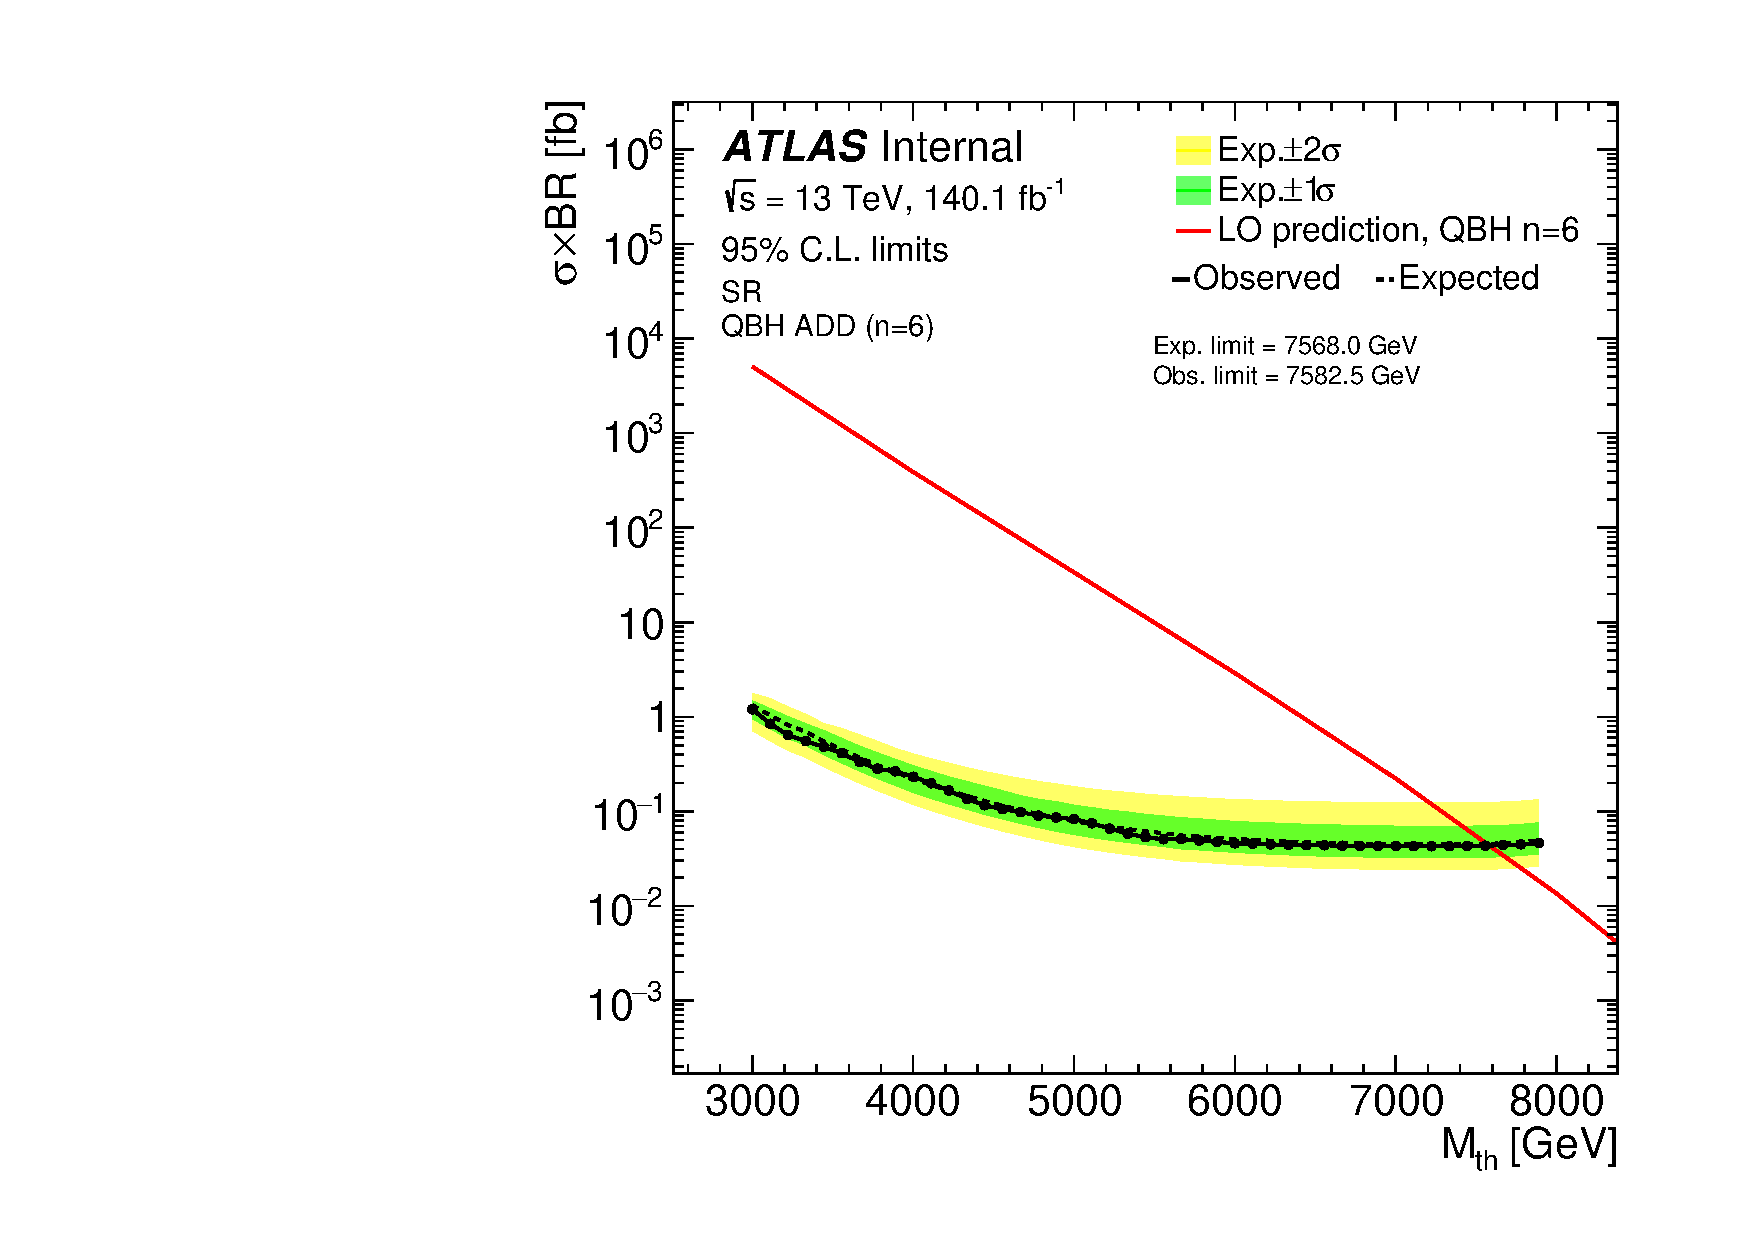
\includegraphics[width=\linewidth]{5_resonances/results/sigbkg/QBH/n6/can__QBH__n6__n6____QBH__SR__Run2}
        \caption{ADD (\(n=6\)) \ac{QBH} model.}
    \end{subfigure}
    \caption{Observed and expected upper limits on the \ac{QBH} signal models. The RS1 model (\(n=1\)) is shown on the left, while the ADD model (\(n=6\)) is presented on the right figure. Observed limits are shown with the black dots and solid line, meanwhile, expected upper limits are represented with the black dashed line, with the correponding \(\pm 1\) and \(\pm 2 \sigma\) uncertainty bands.}
    \label{fig:results:results:bkgsig:results:qbh:limits}
\end{figure}

Again, the present upper limits on the \ac{QBH} masses are the most stringent up to date with the \gammajet final state. Models proposing extra dimensions, whether with warped geometry as proposed by the RS1 model, or with at least two flat extra dimensions as proposed by the ADD model, suggest the formation of \ac{QBH}, and these can be excluded at \(95\%\) up to masses of \(5347.4~\gev\) and \(7590.1~\gev\), respectively.




\paragraph{General Gaussian signals}
\label{paragraph:results:results:bkgsig:results:gaus}


The final signal model considered are general Gaussian shapes. These signals allows for a general and model-agnostic interpretation in this final state. Expected and observed upper limits are computed with Gaussian-shaped resonances, whose width is chosen to take the three following values: \(2\%\), \(7\%\) and \(15\%\) the mass resolution. Unlike the previous models, the reported exclusion limits are on the visible cross section, namely
\begin{equation}
    \sigma_s \times \text{Br} \times A \times \varepsilon,
\end{equation}
as they can be interpreted for any arbitrary signal model that produce a \gammajet resonance of approximately a Gaussian shape in \myj.

For each on of the signal regions considered (SR, SRL, SRC and SRB), the results limits on generic Gaussians with the aforementioned widths are displayed in \Fig{\ref{fig:results:results:bkgsig:results:gaus:limits}}.
In the inclusive SR, the obtained limits show exactly the same structure at low \myj as the other signal models, where a small excess of data events is seen at \(\sim 1800~\gev\) and \(\sim 2500~\gev\).

The sensitivity for narrower resonances is better than that for wider resonances for two reasons: for wide resonances, the same number of signal events is distributed across a larger \myj range, which lowers the signal-to-background ratio in this range. Additionally, the flexibility of the background fit allows it to better adapt to wide signals than to narrow signals, resulting in a larger ambiguity between signal and background events.

From the comparison of different widths, it is also important to note that narrow resonances lead to much more fluctuations on the limits. The reason behind this is that narrow peaks can capture more easily any statistical fluctuation on the data, and these fluctuations are then translated into the limits. Conversely, wider signals lead to much smoother shapes on the observed limits.

\begin{figure}[ht!]
    \centering
    \begin{subfigure}[h]{0.49\linewidth}
        \centering
        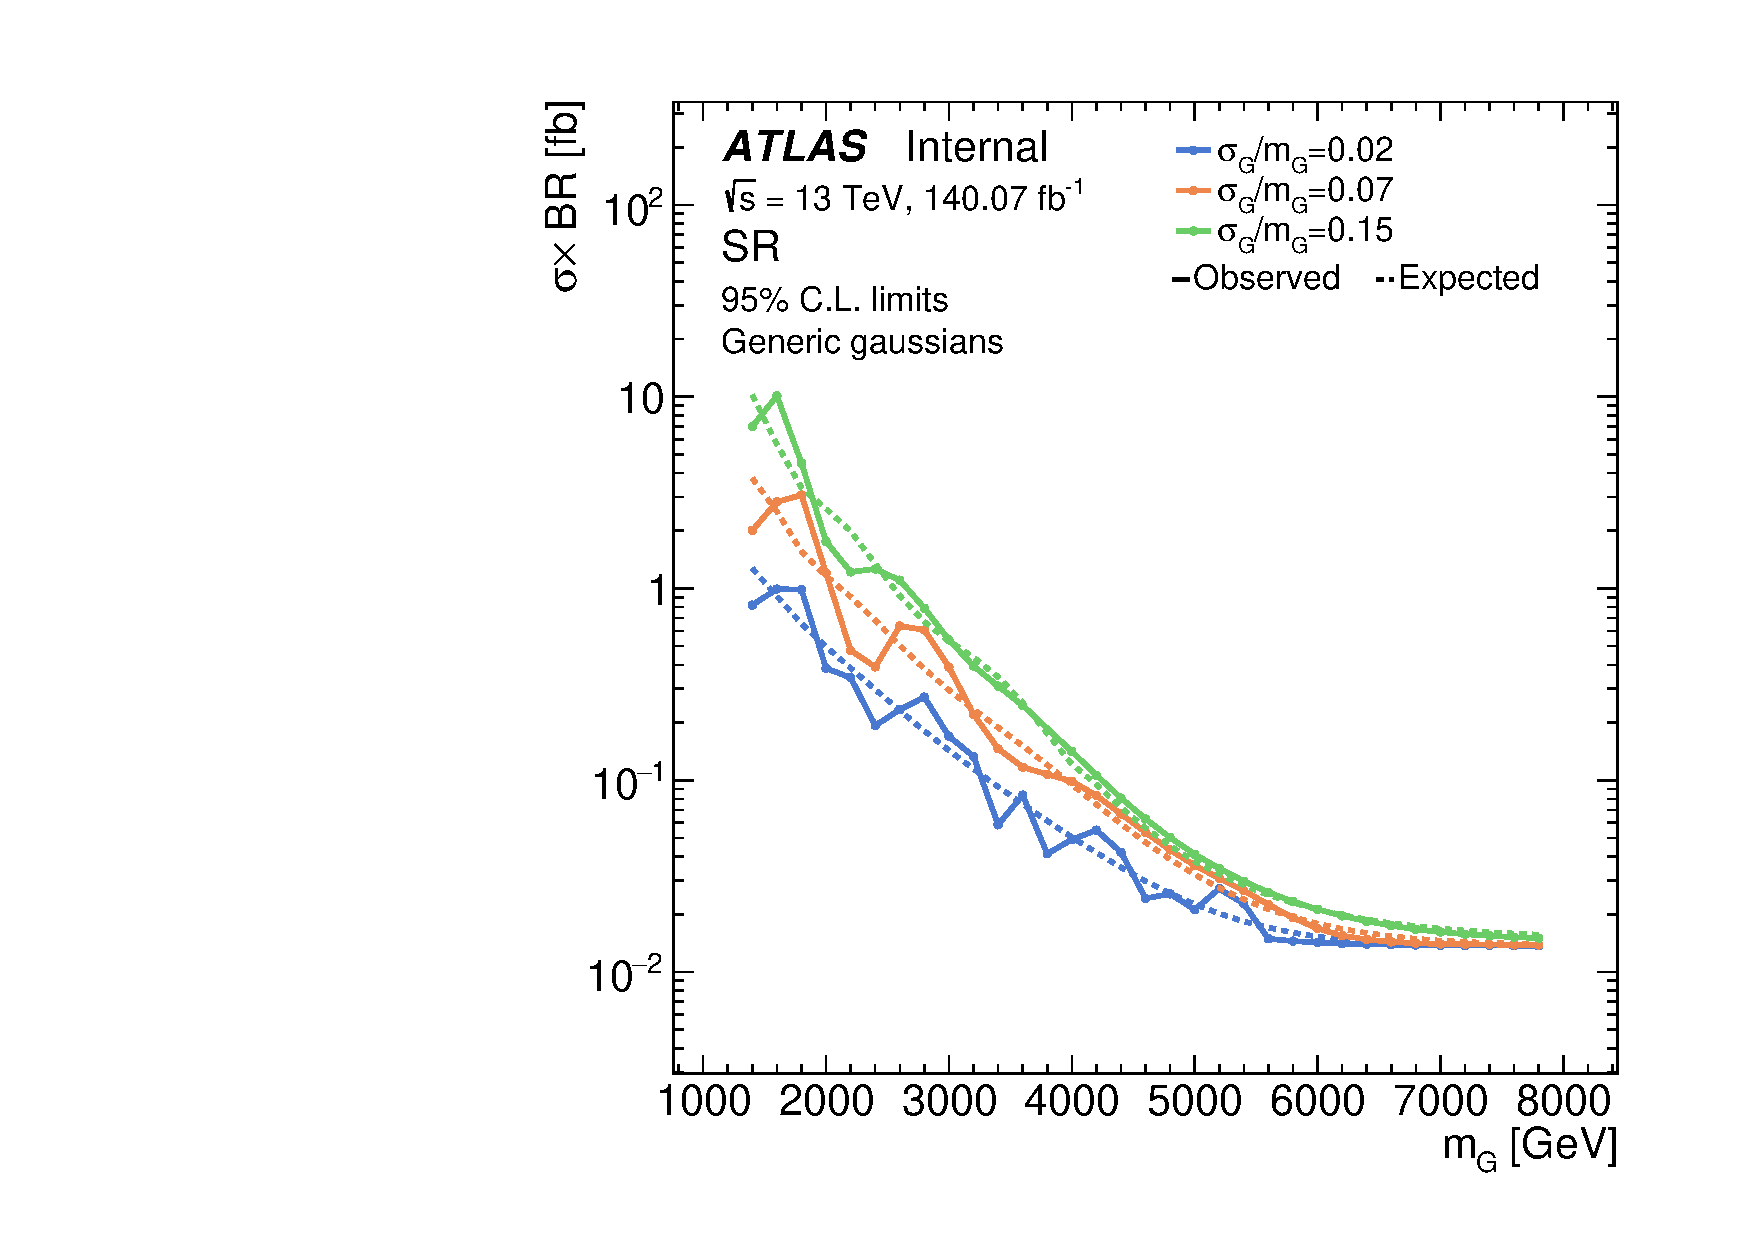
\includegraphics[width=\linewidth]{5_resonances/results/sigbkg/gaus/region/SR/can__gaus__SR__width0p02_width0p07_width0p15__Run2}
        \caption{SR.}
    \end{subfigure}
    \begin{subfigure}[h]{0.49\linewidth}
        \centering
        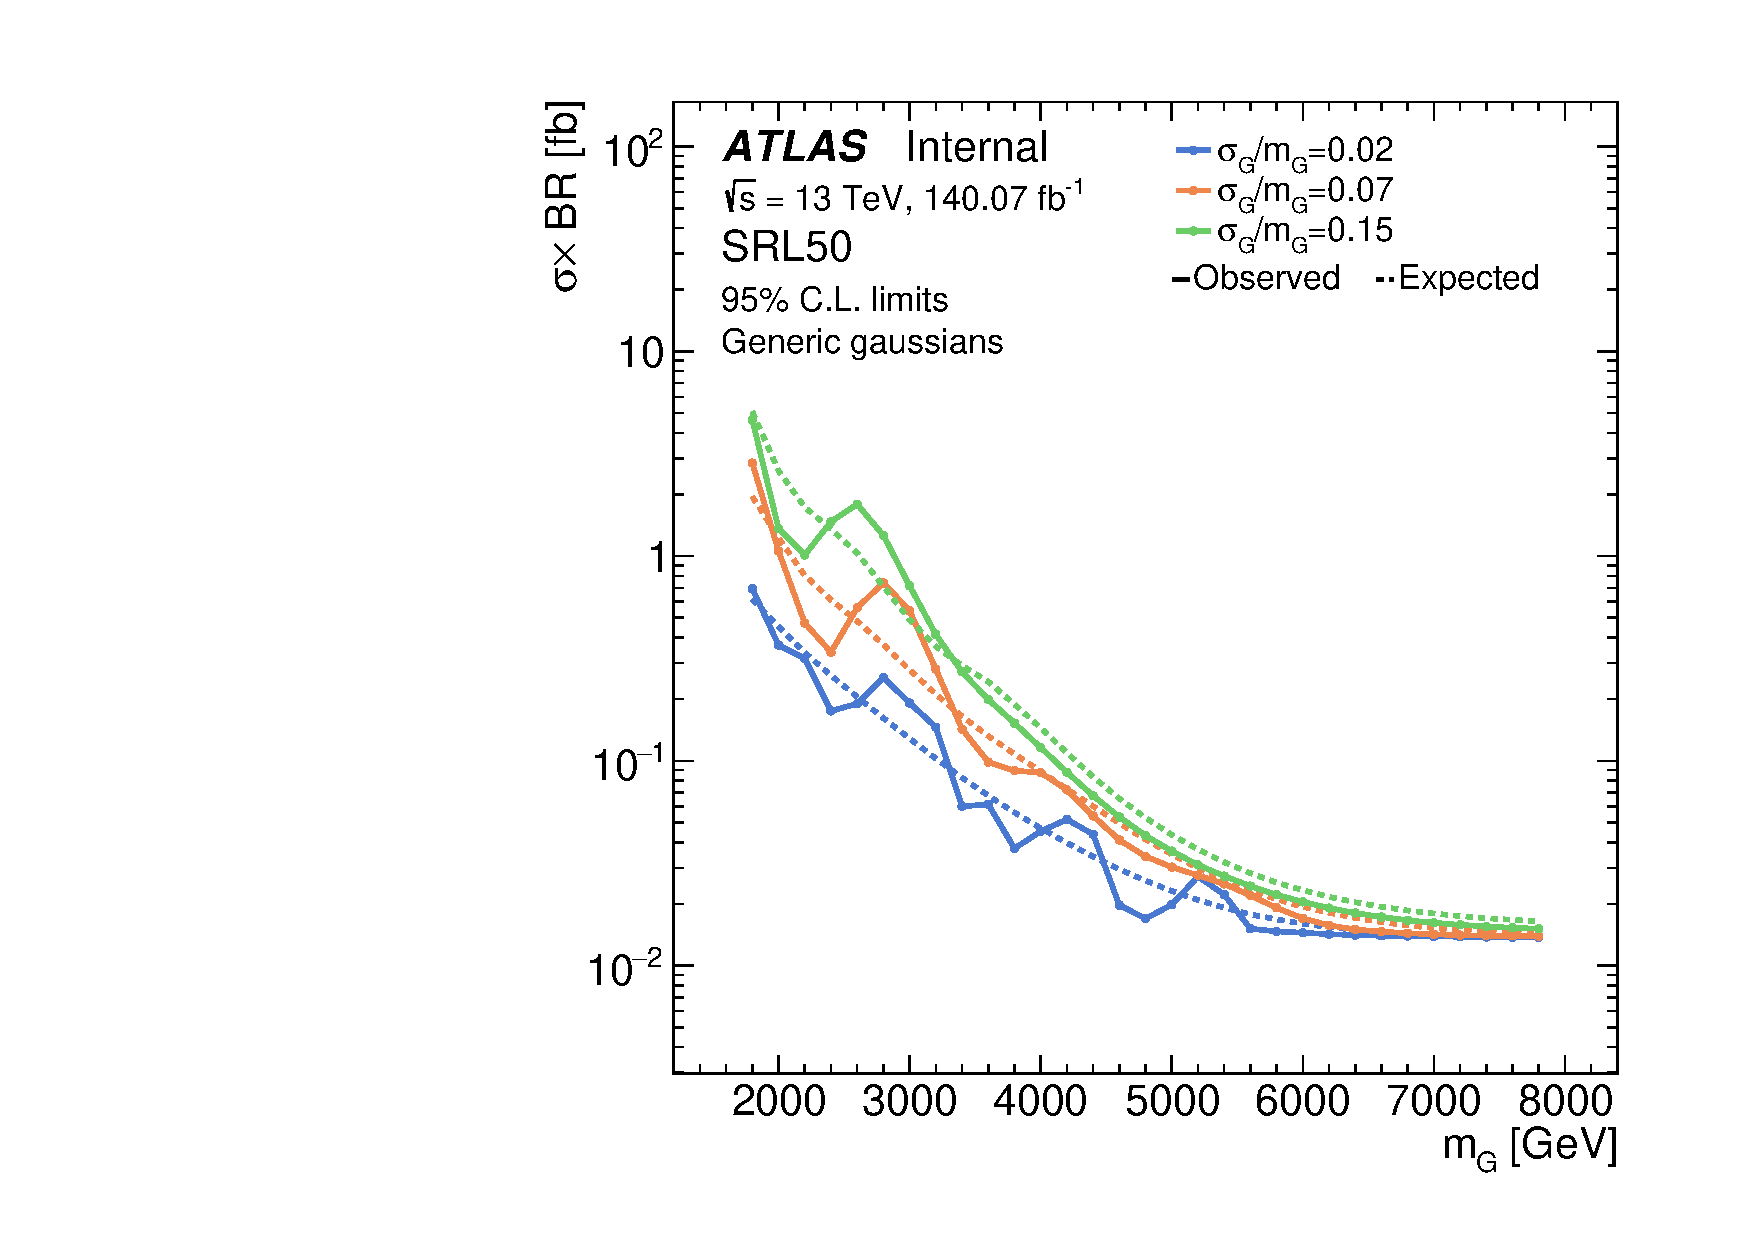
\includegraphics[width=\linewidth]{5_resonances/results/sigbkg/gaus/region/SRL50/can__gaus__SRL50__width0p02_width0p07_width0p15__Run2}
        \caption{SRL50.}
    \end{subfigure}
    \begin{subfigure}[h]{0.49\linewidth}
        \centering
        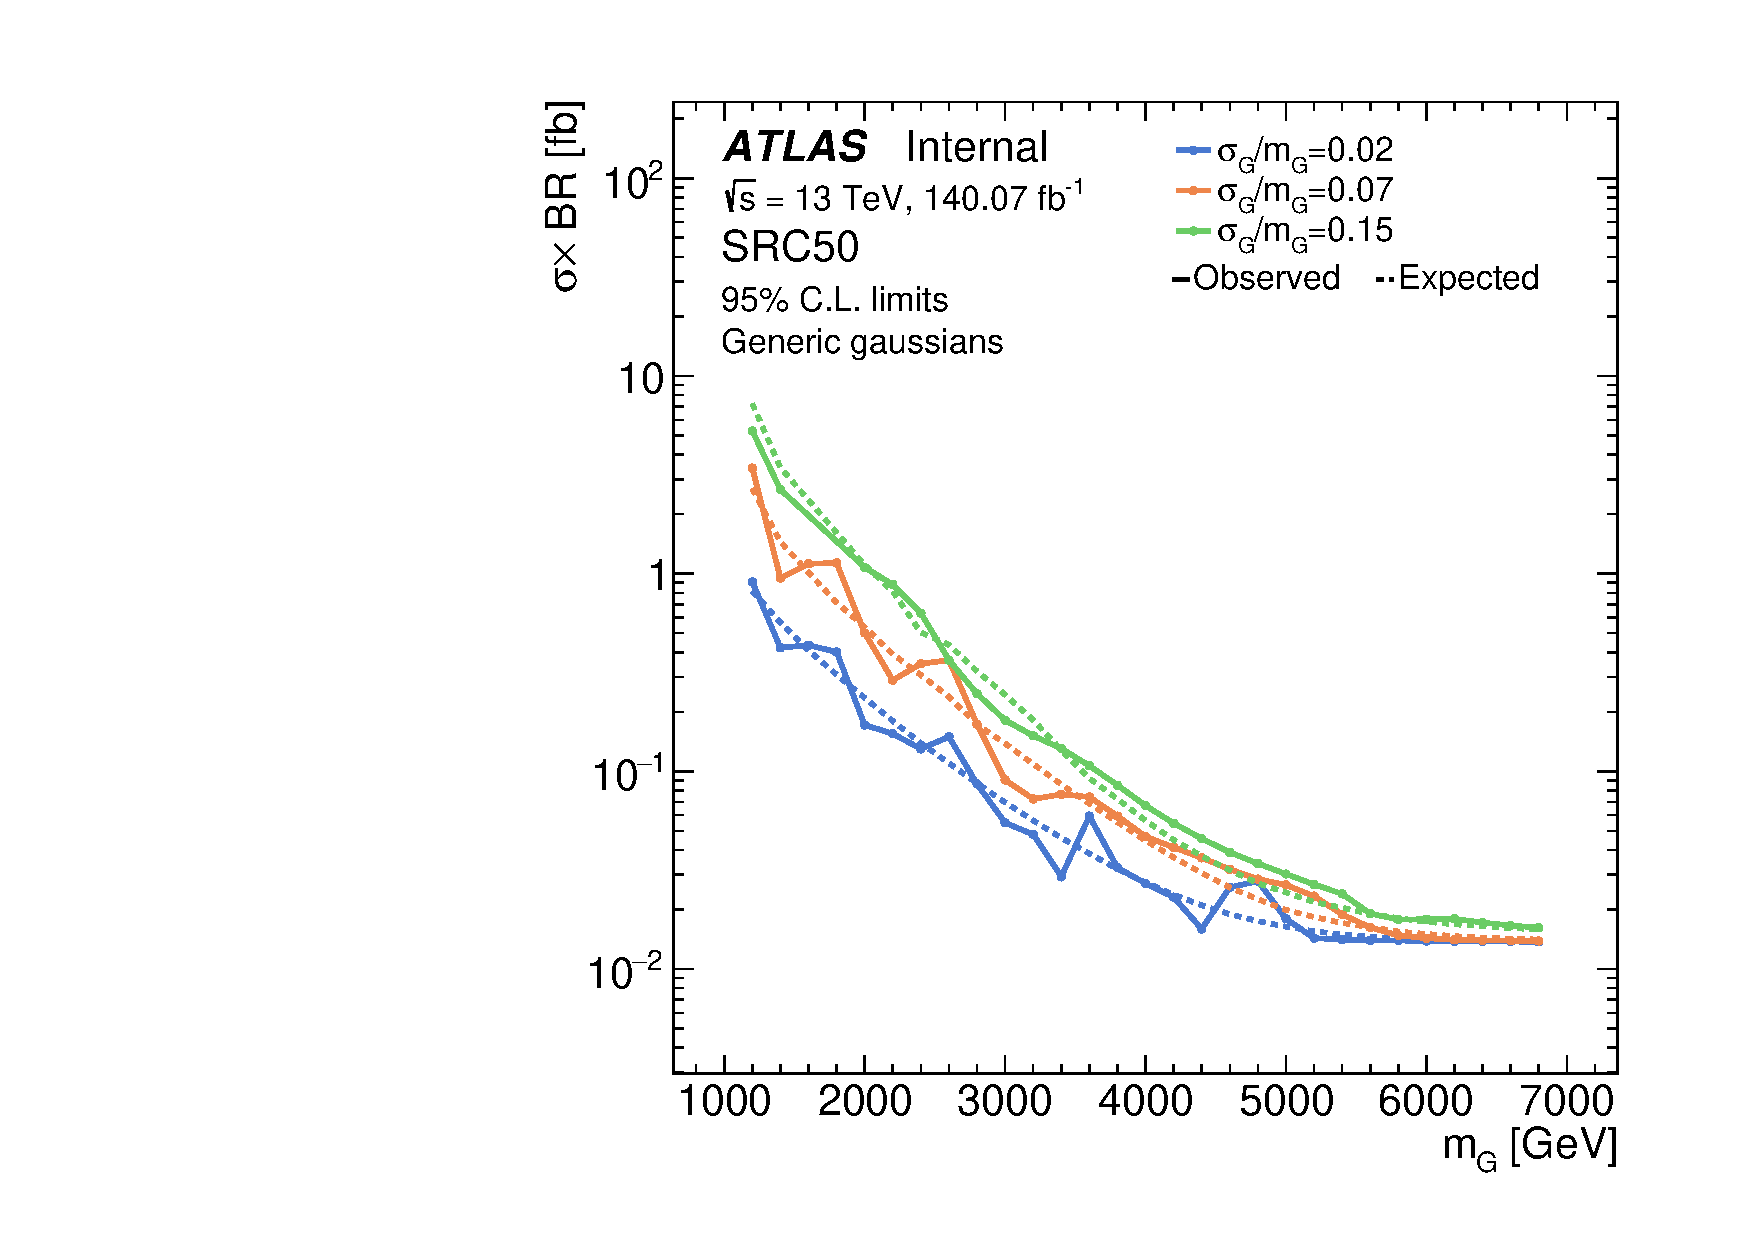
\includegraphics[width=\linewidth]{5_resonances/results/sigbkg/gaus/region/SRC50/can__gaus__SRC50__width0p02_width0p07_width0p15__Run2}
        \caption{SRC.}
    \end{subfigure}
    \begin{subfigure}[h]{0.49\linewidth}
        \centering
        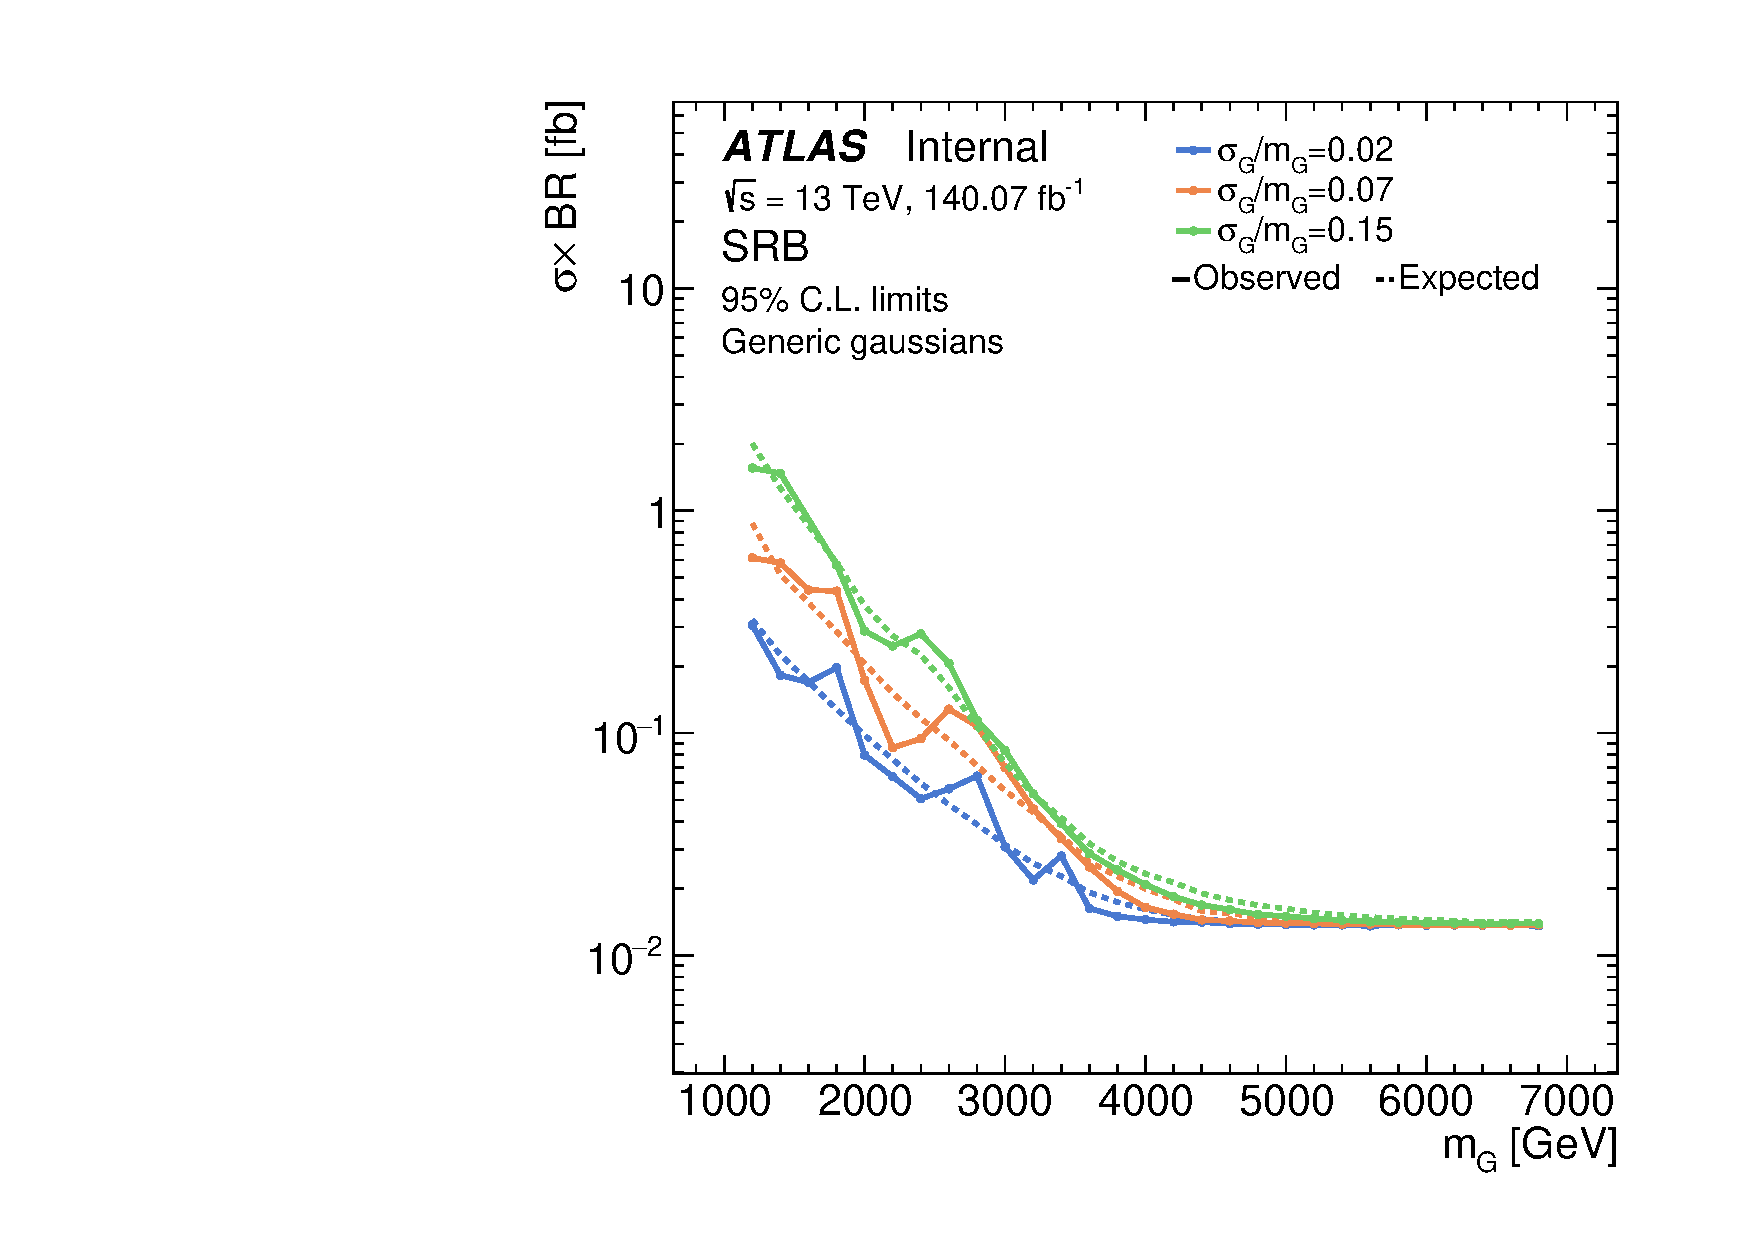
\includegraphics[width=\linewidth]{5_resonances/results/sigbkg/gaus/region/SRB/can__gaus__SRB__width0p02_width0p07_width0p15__Run2}
        \caption{SRB.}
    \end{subfigure}
    \caption{Observed and expected upper lmits on general gaussian signals with three different widths: \(\sigma_G/m_G = 0.02, \, 0.07\) and \(0.15\) in regions SR, SRL, SRC and SRB.}
    \label{fig:results:results:bkgsig:results:gaus:limits}
\end{figure}

\begin{figure}[ht!]
    \centering
    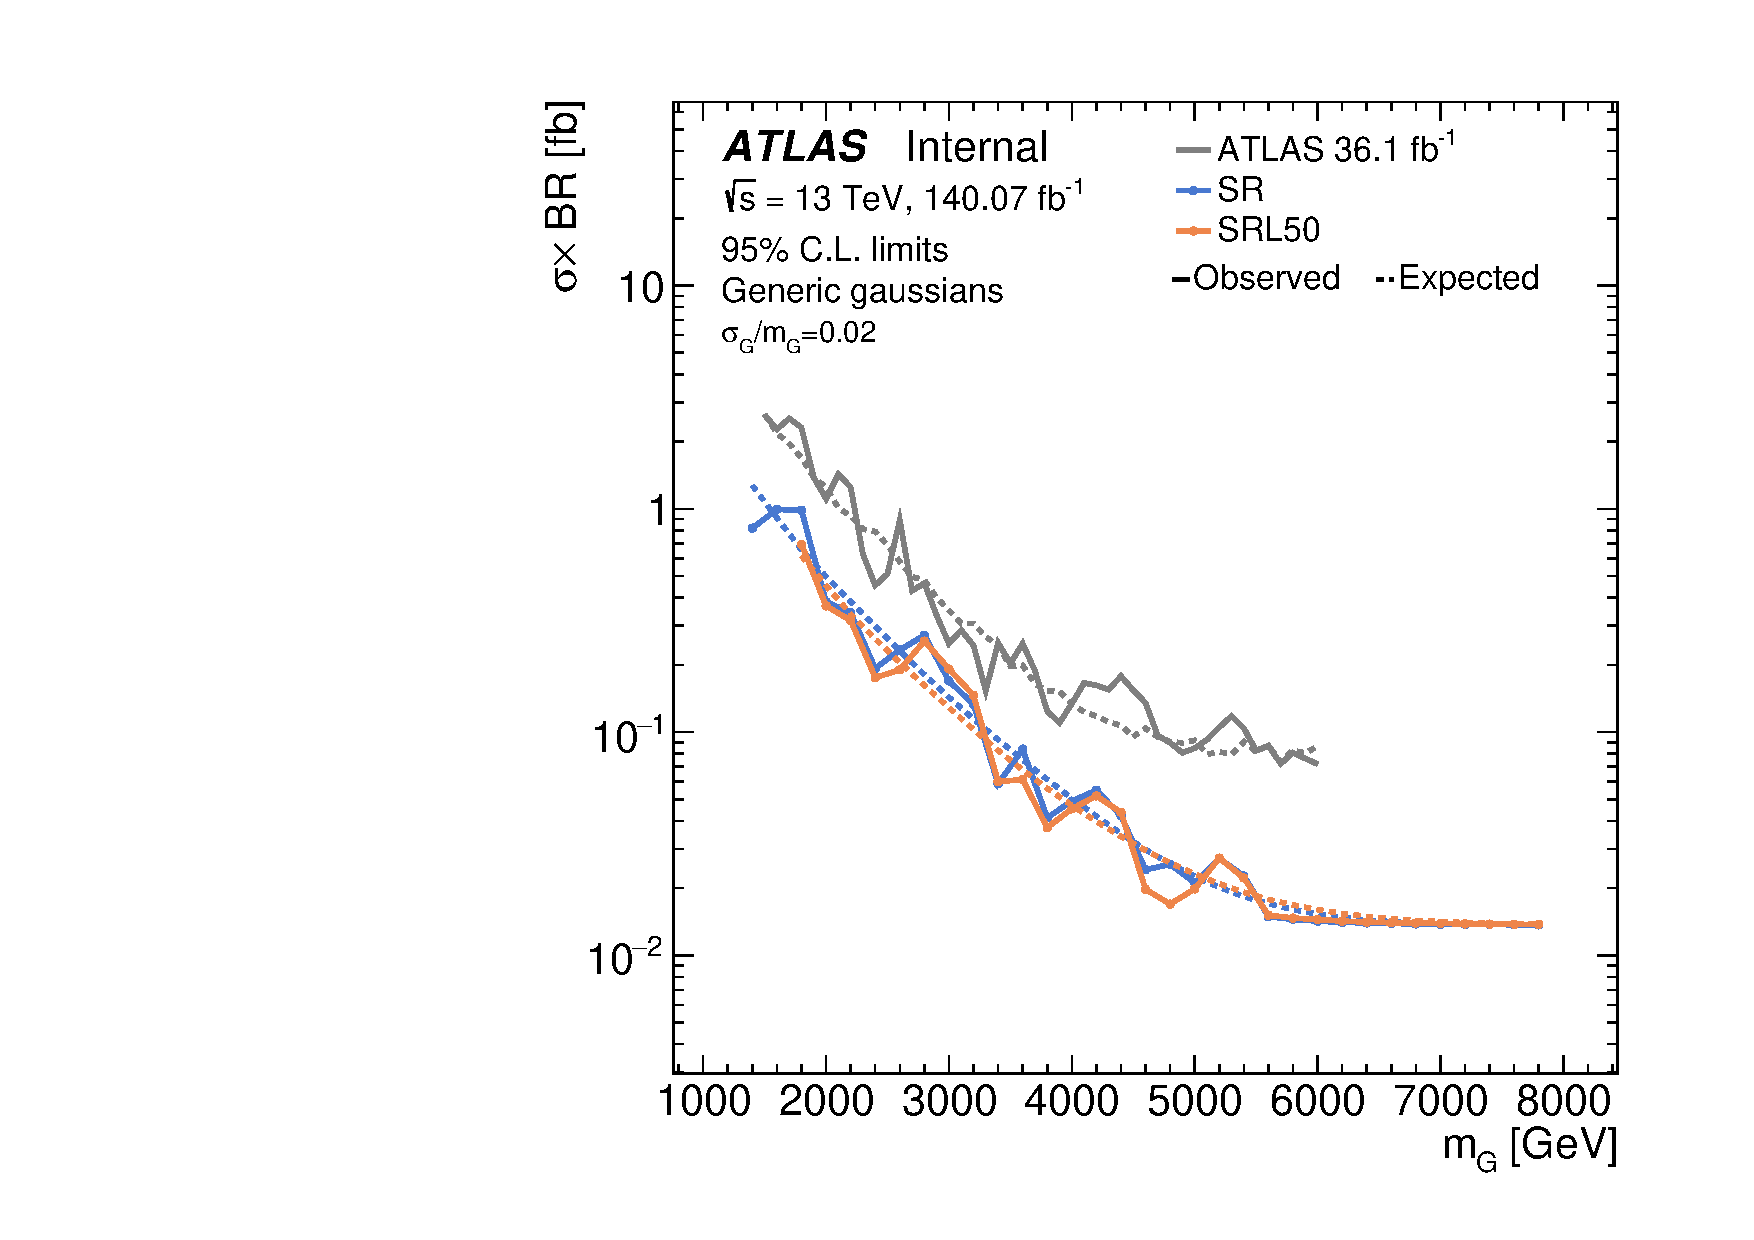
\includegraphics[width=0.6\linewidth]{5_resonances/results/sigbkg/gaus/fixed_param/width0p02/can__gaus__width0p02__SR_SRL50_oldexp_oldobs__Run2}
    \caption{Comparison of the observed and expected limits on Gaussian-shaped resonances of \(2\%\) width obtained in this analysis (blue and orange for the SR and SRL regions, respectively) against the previous \ac{ATLAS} result using 2015-2016 data (grey). The observed limits are shown with the solid line and the expected ones with dashed lines.}
    \label{fig:results:results:bkgsig:results:gaus:limits_comparison_old}
\end{figure}


Finally, in \Fig{\ref{fig:results:results:bkgsig:results:gaus:limits_comparison_old}}, a comparison of the current results with the latest results on gaussian resonances in the \gammajet final state are presentd. The previous search was done using only the 2015+2016 \ac{ATLAS} dataset, leading to a total integrated luminosity of \(36.1~\ifb\). Since the upper limit on the cross-section scales with the luminosity as \(1 / \sqrt{L}\), one would expect a \(\sqrt{140.07} / \sqrt{36.1} \approx 1.96\) improvement on the upper limit. However, as seen from the figures, a higher improvement on the sensitivity is obtained in the current analysis, where the upper limit at \(5500~\gev\) is improved by a factor of approximately 5.3. In consequence, with the current results, by virtue of a more sophisticated background modeling, it is possible to increase the improvements one would get by using more data alone by a factor of \(\sim 2.7\).



%%%%%%%%%%%%%%%%%%%%%%%%%%%%%%%%%%%%%%%%%%%%%%%%%%%%%%%%%%%%%%%%%%%%%%%%%%%%%%%%%%%%%%%%%%%%%%%%%%%%
%%%%%%%%%%%%%%%%%%%%%%%%%%%%%%%%%%%%%%%%%%%%%%%%%%%%%%%%%%%%%%%%%%%%%%%%%%%%%%%%%%%%%%%%%%%%%%%%%%%%
%%%%%%%%%%%%%%%%%%%%%%%%%%%%%%%%%%%%%%%%%%%%%%%%%%%%%%%%%%%%%%%%%%%%%%%%%%%%%%%%%%%%%%%%%%%%%%%%%%%%




%%%%%%%%%%%%%%%%%%%%%%%%%%%%%%%%%%%%%%%%%%%%%%%%%%%%%%%%%%%%%%%%%%%%%%%%%%%%%%%%%%%%%%%%%%%%%%%%%%%%
%%%%%%%%%%%%%%%%%%%%%%%%%%%%%%%%%%%%%%%%%%%%%%%%%%%%%%%%%%%%%%%%%%%%%%%%%%%%%%%%%%%%%%%%%%%%%%%%%%%%
%%%%%%%%%%%%%%%%%%%%%%%%%%%%%%%%%%%%%%%%%%%%%%%%%%%%%%%%%%%%%%%%%%%%%%%%%%%%%%%%%%%%%%%%%%%%%%%%%%%%
%%%%%%%%%%%%%%%%%%%%%%%%%%%%%%%%%%%%%%%%%%%%%%%%%%%%%%%%%%%%%%%%%%%%%%%%%%%%%%%%%%%%%%%%%%%%%%%%%%%%
%%%%%%%%%%%%%%%%%%%%%%%%%%%%%%%%%%%%%%%%%%%%%%%%%%%%%%%%%%%%%%%%%%%%%%%%%%%%%%%%%%%%%%%%%%%%%%%%%%%%
%%%%%%%%%%%%%%%%%%%%%%%%%%%%%%%%%%%%%%%%%%%%%%%%%%%%%%%%%%%%%%%%%%%%%%%%%%%%%%%%%%%%%%%%%%%%%%%%%%%%